\documentclass[10pt]{article}
\usepackage{defaults}
\usepackage{defaults-drawing}
\usetikzlibrary{intersections}

\title{University of Minnesota Physics GWE Solutions}
\author{Justin Willmert}

% Extend the capabilities of enumerations and itemized lists
	\usepackage{enumerate}
% Multicolumn pages
	\usepackage{multicol}
% Circuit drawing
	\usepackage[american,siunitx]{circuitikz}
% Include more unit types
	\DeclareSIUnit{\cal}{cal}
	\DeclareSIUnit{\minute}{min}
	\DeclareSIUnit{\year}{yr}
% Allow subfigures
	\usepackage{subcaption}

% Generate an index of all the GWE problems
\usepackage{makeidx}
	\makeindex
	% Change the index printing so that multicol can balance the columns
	\let\origtheindex\theindex
	\let\origendtheindex\endtheindex
	\def\theindex{%
		\def\twocolumn{\begin{multicols}{2}}%
		\def\onecolumn{}%
		%~ \clearpage
		\origtheindex
	}
	\def\endtheindex{%
		\end{multicols}%
		\origendtheindex
	}

\usepackage[parfill]{parskip}

%% Setup page styles
	% Fancy headers
	\usepackage{fancyhdr}
	\fancypagestyle{plain}{%
		\fancyhf{}	% Clear all headers and footers
		\renewcommand{\headrulewidth}{0pt}
		\renewcommand{\footrulewidth}{0pt}
		\fancyhfoffset{0.25in}
		% Add the page number on the outside of each page and the current
		% exam (section) on the inner header
		\fancyhead[LE,RO]{\sffamily\textbf\thepage}
		\fancyhead[RE,LO]{\sffamily\textbf\leftmark}
		% Also add some information about where to find the source for these
		% solutions in the footer
		\cfoot{%
			\color{black!30!white}
			These solutions are compiled in a \texttt{git} repository available
			at \href{https://github.com/jmert/umn_phys_gwe}
			{https://github.com/jmert/umn\_phys\_gwe}.
		}
	}
	\pagestyle{plain}
	% Since we've added headers and footers which aren't accounted for in the
	% default layout for geometry, setup the new page styles
	\newgeometry{
		twoside     = true,
		includehead = true,
		includefoot = true,
		top         = 0.5in,
		bottom      = 0.5in,
		inner       = 1in,
		outer       = 1in
	}
	% Don't number the sections explicitly, but still use \section, etc
	% (non-starred) so that the TOC is still generated
	\setcounter{secnumdepth}{0}
	% Then have the TOC only show the year and problem numbers without also
	% listing the Question and Answer sections
	\setcounter{tocdepth}{2}

%% Change the heading styles
	\usepackage[sf,bf,compact]{titlesec}
	% Allow use of unstarred sectioning commands without worrying about them
	% adding an unnecessary label before the title. Do this so that the entries
	% are added to the table of contents automatically.
	\titlelabel{}
	\titlespacing*{\section}%
		{-0.25in}		% Create a hanging indent
		{0pt}			% No extra space above the section title
		{0.75em}		% Small amount of space below
	\titlespacing*{\subsection}%
		{-0.125in}		% Create a hanging indent
		{0pt}			% No extra space above the section title
		{0.75em}		% Small amount of space below

%% Make some GWE-specific heading commands
	\makeatletter
	% First, create the requisite counters
	\newcounter{gwe@year}
	\newcounter{gwe@part}
	\newcounter{gwe@prob}[gwe@part]
	% Also an if that signals the first problem in a new exam
	\newif\ifgwe@firstproblem
	% Then add an internal macro which will make the GWE Exam headings
	\newcommand{\gwe@examname}{\relax}
	\xdef\gwe@examsymb{\relax}
	\newcommand{\gwe@exam}[4]{%
		\renewcommand{\gwe@examname}{#1}%
		\xdef\gwe@examsymb{#2}%
		\setcounter{gwe@year}{#3}%
		\setcounter{gwe@part}{#4}%
		\setcounter{gwe@prob}{0}%
		{%
			% Each exam starts on its own page and is its own paragraph
			\clearpage%
			% Generate the title for the command
			\def\gwe@title{%
				\gwe@examname{}~\arabic{gwe@year} Part~\Roman{gwe@part}%
			}%
			% Update the marks so that the headers show which exam we're in,
			% and add ourselves to the TOC
			\markboth{\scshape\gwe@title}{}%
			\section{\gwe@title}
			% Automatically generate a label for every exam of the form
			%     exam:SYYYYP
			% where S is either S or F for spring and fall, respectively,
			%       YYYY is the exam year
			%       P is the part number (I or II)
			\edef\@currentlabelname{\gwe@title}%
			\edef\gwe@label{\gwe@examsymb\arabic{gwe@year}\Roman{gwe@part}}%
			\label{exam:\gwe@label}%
		}%
		% Signal to \problem that it is the first after a new exam
		\gwe@firstproblemtrue%
	}%
	% Next, add convenience wrappers to quickly define the Spring and Fall
	% exams.
	\newcommand{\fallexam}[2]{\gwe@exam{Fall}{F}{#1}{#2}}%
	\newcommand{\springexam}[2]{\gwe@exam{Spring}{S}{#1}{#2}}%
	% Finally, provide a heading for each problem
	\newcommand{\problem}[1]{%
		\setcounter{gwe@prob}{#1}%
		% Reset the equation numbering counter
		\setcounter{equation}{0}%
		{%
			% New problems also start on their own pages if it's not the first
			% in the exam (still want to share the page with exam title)
			\ifgwe@firstproblem%
				\global\gwe@firstproblemfalse%
			\else%
				\clearpage%
			\fi%
			% Generate the title for the command
			\def\gwe@title{%
				Problem~\arabic{gwe@prob}%
			}%
			\def\gwe@fulltitle{%
				\gwe@examname{}~\arabic{gwe@year} Part~\Roman{gwe@part}, %
				\gwe@title%
			}%
			\subsection{\gwe@title}
			% Automatically generate a label for every problem of the form
			%     prob:SYYYYPNN
			% where S is either S or F for spring and fall, respectively,
			%       YYYY is the exam year
			%       P is the part number (I or II)
			%       NN is the problem number including leading zero
			\edef\nn{\ifnum\value{gwe@prob}<10 0\fi\thegwe@prob}%
			\edef\@currentlabelname{\gwe@fulltitle}%
			\edef\gwe@label{\gwe@examsymb\arabic{gwe@year}\Roman{gwe@part}\nn}%
			\label{prob:\gwe@label}%
		}%
	}
	% Set the equation numbering system:
	\renewcommand{\theequation}{%
		\gwe@examsymb\arabic{gwe@year} \Roman{gwe@part} \arabic{gwe@prob}.\arabic{equation}%
	}
	% hyperref makes use of special macros to set the internal
	% cross-referencing names, so mangle those so that they're unique for
	% problems and equations.
	%
	% Must be done after hyperref is loaded at the end of the preamble by
	% defaults package, so wrap in \AtEndPreamble{} to delay execution.
	\AtEndPreamble{
		\renewcommand{\theHsection}{%
			\gwe@examsymb\arabic{gwe@year}\Roman{gwe@part}%
		}
		\renewcommand{\theHsubsection}{%
			\theHsection.\arabic{gwe@prob}%
		}
		\renewcommand{\theHequation}{%
			\theHsubsection.\arabic{equation}%
		}
	}
	\makeatother

%% Convenience macros
	% Script L used for Lagrangian
	\newcommand{\sL}{\ensuremath{\mathcal L}}
	% Derivative shortcut
	\newcommand{\dd}{\ensuremath{\,\mathrm{d}}}
	% Quantum bra-ket notation can be annoying, so make that more convenient
	% to type
	% · First, have macros for lone bras and kets
	\newcommand{\bra}[1]{\ensuremath{\left\langle #1 \right|}}
	\newcommand{\ket}[1]{\ensuremath{\left| #1 \right\rangle}}
	% · Next, make a bra-ket pair so that all three < | > are the same sizes
	\newcommand{\braket}[2]{\ensuremath{%
		\left\langle #1 \middle| #2 \right\rangle%
	}}
	% · Also have one that can sandwich an operator expression in the middle.
	\newcommand{\braopket}[3]{\ensuremath{%
		\left\langle #1 \middle| #2 \middle| #3 \right\rangle
	}}
	% · Finally, expectation values
	\newcommand{\expect}[1]{\ensuremath{\left\langle #1 \right\rangle}}

\begin{document}

\begingroup
	% Use smaller fonts for the TOC and index
	\small
	% Patch the table of contents to use double columns. Needs to be done here
	% because something else redefines \@starttoc when the document begins
	% (probably hyperref...)
	\makeatletter
	\let\origstarttoc\@starttoc
	\renewcommand*{\@starttoc}[1]{%
		\begin{multicols}{2}%
			\origstarttoc{#1}%
		\end{multicols}%
	}
	\makeatother
	\tableofcontents

	% Print the Index
	\printindex
	\clearpage
\endgroup

\fallexam{2000}{1}
%%%%%%%%%%%%%%%%%%%%%%%%%%%%%%%%%%%%%%%%%%%%%%%%%%%%%%%%%%%%%%%%%%%%%%%%%%%%%%%
%%%% Problem 8
%%%%%%%%%%%%%%%%%%%%%%%%%%%%%%%%%%%%%%%%%%%%%%%%%%%%%%%%%%%%%%%%%%%%%%%%%%%%%%%
\problem{8}
\subsubsection{Question}
% Keywords
	\index{thermodynamics!Nitrogen velocity}

Estimate (a) the average speed (in \si{\m\per\s}) and (b) the mean free path
(in \si{\m}) of a nitrogen molecule in this room.

\subsubsection{Answer}

\begin{enumerate}[(a)]
	\item
		We relate the kinetic energy of an $N_2$ molecule with the thermal
		energy by the equipartition theorem. Since there are 3 translational
		degrees of freedom,
		\begin{align*}
			\frac 12 mv² &= \frac 32 k_B T \\
			v &= \sqrt{\frac{3 k_B T}{m}}
		\end{align*}
		The mass of the molecule is twice that of a single nitrogen atom
		which is itself about 14 proton masses. Therefore
		\begin{empheq}[box=\fbox]{align}
			v &≈ \sqrt{\frac{3 k_B T}{28 m_p}} \\
			v &≈ \SI{515}{\m\per\s}
		\end{empheq}
	\item
		Two particles collide if they come within $2r₀$ of each other where
		$r₀$ is the typical radius of the particle. For diatomic nitrogen,
		we assume $r₀ ≈ 2a₀$ where $a₀$ is the Bohr radius. Then in the time
		$τ$ that the particle is moving at velocity $⟨v⟩$, the particle can
		collide with any other particle within the swept-out volume
		\begin{align*}
			\mathcal V &= π(2r₀)² ⋅ ⟨v⟩τ
		\end{align*}
		Since there are $n$ particles per unit volume, there are $\mathcal N$
		atoms to collide with:
		\begin{align*}
			\mathcal N &= n\mathcal V = 4πn{r₀}² ⟨v⟩τ
		\end{align*}
		On average then, there are $\mathcal N$ collisions per length $⟨v⟩τ$
		traversed, or in its reciprocal form, the mean free path $λ$ is
		\begin{align*}
			λ &= \frac{1}{4πn{r₀}²}
		\end{align*}
		To estimate the particle density, consider the ideal gas law
		$PV=Nk_BT$. We can assume atmospheric pressure at room temperature,
		so the density is
		\begin{align*}
			n &= \frac N V = \frac{P}{k_B T}
		\end{align*}
		Putting it all together,
		\begin{empheq}[box=\fbox]{align}
			λ &≈ \frac{k_B T}{4π{r₀}²P} \\
			{}&≈ \SI{2.90e-7}{\m}
		\end{empheq}
\end{enumerate}


\springexam{2000}{1}
%%%%%%%%%%%%%%%%%%%%%%%%%%%%%%%%%%%%%%%%%%%%%%%%%%%%%%%%%%%%%%%%%%%%%%%%%%%%%%%
%%%% Problem 1
%%%%%%%%%%%%%%%%%%%%%%%%%%%%%%%%%%%%%%%%%%%%%%%%%%%%%%%%%%%%%%%%%%%%%%%%%%%%%%%
\problem{1}
\subsubsection{Question}
% Keywords
	\index{mechanics!Energy loss in orbital descent}

A satellite of mass $m = \SI{500}{\kg}$ is in a circular orbit at an
altitude $h = \SI{150}{\km}$ above the Earth's surface. As a result of air
friction, the satellite's orbit degrades. Protected by a heat shield, the
satellite eventually impacts with a velocity of $\SI{2}{\km\per\s}$. How
much energy (in Joules) was released as heat in the process?

\subsubsection{Answer}

The solution method will be a simple energy balance equation. In its initial
state, the satellite had gravitation potential energy that contributed to
its energy equal to
\begin{align*}
    V_0 &= \frac{GM_E m}{R_E + h}
\end{align*}
where $M_E$ and $R_E$ are the mass and radius of the Earth. The kinetic energy
can be determined by making use of simple circle relations. The centripetal
force must be provided by the gravitation force, so
\begin{align*}
    \frac{{v_0}^2}{R_E + h} &= \frac{GM_E}{(R_E + h)^2} \\
    v_0 &= \sqrt{\frac{GM_E}{R_E + h}}
\end{align*}
making the initial kinetic energy
\begin{align*}
    T_0 &= \frac{GM_E m}{2(R_E + h)}
\end{align*}

In it's final state, the satellite consists of it's final given velocity's
kinetic energy and more gravitational potential energy (with respect to the
center of the Earth). They are given by
\begin{align*}
    T_f &= \frac 12 m{v_f}^2 \\
    V_f &= \frac{GM_E m}{R_E}
\end{align*}
By conservation of energy, any energy different must result from the loss
of energy between the initial and final states, so the lost energy
$E_\mathrm{loss}$ is
\begin{align*}
    E_\mathrm{loss} &= T_0 + V_0 - T_f - V_f \\
    {} &= \frac{GM_E m}{R_E(R_E + h)}(R_E - 2h) - \frac 12 m{v_f}^2
\end{align*}
Plugging in all given quantities and constants, we have that
\begin{align}
    \boxed{
    E_\mathrm{loss} = \SI{2.816e10}{\J} = \SI{28.16}{\giga\J}
    }
\end{align}

%%%%%%%%%%%%%%%%%%%%%%%%%%%%%%%%%%%%%%%%%%%%%%%%%%%%%%%%%%%%%%%%%%%%%%%%%%%%%%%
%%%% Problem 2
%%%%%%%%%%%%%%%%%%%%%%%%%%%%%%%%%%%%%%%%%%%%%%%%%%%%%%%%%%%%%%%%%%%%%%%%%%%%%%%
\problem{2}
\subsubsection{Question}
% Keywords
    \index{mechanics!Recoiling iron}

What is the velocity of recoil of an ${}^{57}\mathrm{Fe}$ nucleus that emits
a \SI{100}{\keV} photon, both in units of the speed of light in vacuum and in
meters per second.

\subsubsection{Answer}

In the initial state observed from the iron atom's rest frame, the momentum
is zero. After the emission, the photon has a momentum of $p_\gamma = E_\gamma/c$ and
consequently, the nucleus must recoil with momentum $p_{Fe} = -p_\gamma$. Knowing
that the energy is non-relativistic, then
\begin{align*}
    m_{Fe}v_{Fe} &= \frac{E_\gamma }{c} \\
    v_{Fe} &= \frac{E_\gamma }{57m_p c}
\end{align*}
where we've approximate the mass of the iron atom by a multiple of the proton
mass. Plugging in the numbers
\begin{align}
    \boxed{ v_{Fe} = \SI{561.4}{\m\per\s} }
\end{align}
or in units of $c$
\begin{align}
    \boxed{ v_{Fe} = \SI{1.87e-6}{c} }
\end{align}

%%%%%%%%%%%%%%%%%%%%%%%%%%%%%%%%%%%%%%%%%%%%%%%%%%%%%%%%%%%%%%%%%%%%%%%%%%%%%%%
%%%% Problem 3
%%%%%%%%%%%%%%%%%%%%%%%%%%%%%%%%%%%%%%%%%%%%%%%%%%%%%%%%%%%%%%%%%%%%%%%%%%%%%%%
\problem{3}
\subsubsection{Question}
% Keywords
    \index{electrodynamics!Voltage and phase in an RL circuit}
    \index{circuits!Voltage and phase in an RL circuit}

A resistance $R$ and an inductance $L$ are connected in series, and an
alternating voltage $V_0\cos {\omega} t$ is impressed across the combination. The
resulting steady state voltage across the resistance can be written as $V_R
\cos({\omega} t + \beta)$. Find $V_R$ and $\beta$, assuming both $V_0$ and $V_R$ to be
positive.

\subsubsection{Answer}

The problem is simplified by constucting the solution using complex voltages
and currents and recovering the correct component at the end. Since the
source voltage is a cosine, the real component will be kept at the end.

The complex impedance for a resistor is simply the resitance itself, so $Z_R
= R$. For the inductor, it is $Z_L = i{\omega} L$. We then use the complex
impedances together with Ohm's Law and the first Kirchoff rule to solve for
the complex current $I$.
\begin{align*}
    V_0e^{i{\omega} t} &= IR + i{\omega} LI \\
    I &= \frac{V_0}{R+i{\omega} L} e^{i{\omega} t}
\end{align*}
Then by inserting this solution into the voltage law for inductors, we can
solve for the complex voltage across the inductor.
\begin{align*}
    V_L &= L\frac{dI}{dt} \\
    V_L &= V_0 \frac{i{\omega} L}{R+i{\omega} L} e^{i{\omega} t}
\end{align*}

The voltage drops across the resistor and inductor must equal the impressed
voltage, so we can solve for the unknown voltage across the resistor.
\begin{align*}
    V_0e^{i{\omega} t} &= V + V_L \\
    V &= V_0e^{i{\omega} t} - V_0\frac{i{\omega} L}{R+i{\omega} L}e^{i{\omega} t} \\
    V &= V_0 (\frac{R^2 - i{\omega} RL}{R^2 + {\omega}^2L^2}) e^{i{\omega} t}
\end{align*}
In order to make taking the real component simpler, we put the term in
parentheses in complex exponential form according to the relation $z =
|z|e^{i \arg z}$.
\begin{align*}
    \left| \frac{R^2 - i{\omega} RL}{R^2 + {\omega}^2L^2} \right| &=
	\frac{R\sqrt{R^2 + {\omega}^2L^2}}{R^2 + {\omega}^2L^2}
    \\
    \arg (\frac{R^2 - i{\omega} RL}{R^2 + {\omega}^2L^2}) &= \arctan(-\frac{{\omega} L}{R})
\end{align*}
Therefore the voltage across the resistor has the form
\begin{align*}
    V &= V_0 \frac{R\sqrt{R^2 + {\omega}^2L^2}}{R^2 + {\omega}^2L^2} e^{i{\omega} t + \arctan(-{\omega} L/R)} \\
    V &= V_R e^{i{\omega} t + i\beta} \\
    \Re\{V\} &= V_R \cos({\omega} t + \beta)
\end{align*}
where
\begin{align}
    \boxed{ V_R = V_0 \frac{R\sqrt{R^2 + {\omega}^2L^2}}{R^2 + {\omega}^2L^2} }
    \quad\quad
    \boxed{ \beta = \arctan(-\frac{{\omega} L}{R}) \vphantom{\frac{\sqrt{R}}{R}} }
\end{align}

%%%%%%%%%%%%%%%%%%%%%%%%%%%%%%%%%%%%%%%%%%%%%%%%%%%%%%%%%%%%%%%%%%%%%%%%%%%%%%%
%%%% Problem 4
%%%%%%%%%%%%%%%%%%%%%%%%%%%%%%%%%%%%%%%%%%%%%%%%%%%%%%%%%%%%%%%%%%%%%%%%%%%%%%%
\problem{4}
\subsubsection{Question}
% Keywords
    \index{electrodynamics!Flux through a loop}

Find the magnetic flux through a square loop of side $a$ due to current $I$ in
a long straight wire. The geometry is as follows: the wire is coplanar with the
loop and runs parallel to the loop's closest side, at a distance $b$ away.
Write your result as a formula in SI units.

\subsubsection{Answer}

By Ampère's law in integral form, the magnetic field at a radial distance $r$
away from the wire is given by
\begin{align*}
    \vec B = \frac{{\mu}_0I}{2{\pi} r} \hat \phi 
\end{align*}
The flux is then the total magnetic field through the loop. Integrating by
lines of length $a$,
\begin{align*}
    \phi  = a \int_b^{a+b} \frac{{\mu}_0I}{2{\pi} r} dr \\
    \boxed{\phi  = \frac{{\mu}_0Ia}{2{\pi}}\ln(\frac{a+b}{a})}
\end{align*}

%%%%%%%%%%%%%%%%%%%%%%%%%%%%%%%%%%%%%%%%%%%%%%%%%%%%%%%%%%%%%%%%%%%%%%%%%%%%%%%
%%%% Problem 6
%%%%%%%%%%%%%%%%%%%%%%%%%%%%%%%%%%%%%%%%%%%%%%%%%%%%%%%%%%%%%%%%%%%%%%%%%%%%%%%
\problem{6}
\subsubsection{Question}
% Keywords
    \index{mathematics!Complex contour integration}

By actually evaluating the integral, show that
\begin{align*}
    \int_0^\infty  \frac{\cos x}{1 + x^2}\,dx &= \frac{{\pi}}{2e}
\end{align*}

\subsubsection{Answer}

Note that the integrand, so start by changing the limits of integration
\begin{align*}
    \int_0^\infty  \frac{\cos x}{1 + x^2}\,dx &=
	\frac 12 \int_{-\infty }^\infty  \frac{\cos x}{1 + x^2}\,dx
\intertext{Then expand the cosine into is complex exponential definition}
    {} &= \frac 14 (\int_{-\infty }^\infty  \frac{e^{ix}}{1 + x^2}\,dx +
	\int_{-\infty }^\infty  \frac{e^{-ix}}{1 + x^2}\,dx) \\
    {} &= \frac 14 (\int_{-\infty }^\infty  \frac{e^{ix}}{(x+i)(x-i)}\,dx +
	\int_{-\infty }^\infty  \frac{e^{-ix}}{(x+i)(x-i)}\,dx)
\intertext{Complex contour integration lets us evaluate the integrals as
limits of the coefficient of a pole as it approaches the pole, so}
    {} &= \frac 14 (2{\pi} i \cdot  \lim_{z\rightarrow i}(\frac{e^{iz}}{z+i}) - 2{\pi} i  \cdot 
	\lim_{z\rightarrow -i}(\frac{e^{-iz}}{z-i}))
\end{align*}
After simplifying,
\begin{align}
    \boxed{
    \int_0^\infty  \frac{\cos x}{1 + x^2}\,dx = \frac{{\pi}}{2e}
    }
\end{align}

%%%%%%%%%%%%%%%%%%%%%%%%%%%%%%%%%%%%%%%%%%%%%%%%%%%%%%%%%%%%%%%%%%%%%%%%%%%%%%%
%%%% Problem 7
%%%%%%%%%%%%%%%%%%%%%%%%%%%%%%%%%%%%%%%%%%%%%%%%%%%%%%%%%%%%%%%%%%%%%%%%%%%%%%%
\problem{7}
\subsubsection{Question}
% Keywords
    \index{dimensional analysis!High-velocity drag force}

The drag force on a very high speed object of area $A$, passing through a gas
of density $\rho$ at a velocity $v$ is expected to be of the form
\begin{align*}
    \text{Force} \sim A^r \rho^s v^t
\end{align*}
Determine the value of the exponents $r$, $s$, and $t$.

\subsubsection{Answer}

Force needs to have a unit of inverse time squared, therefore $v$ as the only
variable with a time unit sets $t = 2$. Similarly, $\rho $ is the only one with
a mass term, so we also immediately know that $s = 1$. That leaves
\begin{align*}
    \left[ \frac{\text{mass}\cdot \text{distance}}{\text{time}^2} \right]
	&= \left[ \frac{\text{mass}}{\text{distance}\cdot \text{time}^2} \right]
	\left[ \text{distance} \right]^r
\end{align*}
Therefore to have the two side have compatible units, $r = 2$.
\begin{align*}
    \boxed{ r = 2,\quad s = 1,\quad t = 2}
\end{align*}

%%%%%%%%%%%%%%%%%%%%%%%%%%%%%%%%%%%%%%%%%%%%%%%%%%%%%%%%%%%%%%%%%%%%%%%%%%%%%%%
%%%% Problem 9
%%%%%%%%%%%%%%%%%%%%%%%%%%%%%%%%%%%%%%%%%%%%%%%%%%%%%%%%%%%%%%%%%%%%%%%%%%%%%%%
\problem{9}
\subsubsection{Question}
% Keywords
    \index{mechanics!Shallow-water wave group velocity}
    \index{waves!Shallow-water wave group velocity}

For waves in shallow water, the relation between frequency $\nu $ and wavelength
${\lambda}$ is
\begin{align*}
    \nu  &= (\frac{2{\pi} T}{\rho {\lambda}^3 })^{1/2}
\end{align*}
where $\rho $ and $T$ are the density and surface tension of water. What is the
group velocity of these waves?

\subsubsection{Answer}

Transforming relation given to use the angular frequency ${\omega} = 2{\pi}\nu $ and
wave number $k = 2{\pi}/{\lambda}$,
\begin{align*}
    {\omega} &= \sqrt{ \frac{k^3 T}{\rho } }
\end{align*}
Then the group velocity is simply the partial derivative with respect to $k$:
\begin{align*}
    v_g &= \frac{\partial {\omega}}{\partial k} = \frac 32 \sqrt{\frac{kT}{\rho }}
\end{align*}
Putting this back into the form which involves only $\nu $ and ${\lambda}$, we arrive at
the answer
\begin{align}
    \boxed{ v_g = \frac 32 \sqrt{\frac{2{\pi} T}{\rho {\lambda}}} }
\end{align}

%%%%%%%%%%%%%%%%%%%%%%%%%%%%%%%%%%%%%%%%%%%%%%%%%%%%%%%%%%%%%%%%%%%%%%%%%%%%%%%
%%%% Problem 10
%%%%%%%%%%%%%%%%%%%%%%%%%%%%%%%%%%%%%%%%%%%%%%%%%%%%%%%%%%%%%%%%%%%%%%%%%%%%%%%
\problem{10}
\subsubsection{Question}
% Keywords
    \index{mathematics!Eigenvalues and eigenvectors}

Find the eigenvalues and corresponding eigenvectors (which need \emph{not} be
normalized) of the following matrix:
\begin{align*}
    M = \begin{bmatrix}
	1 & 0 & -i \\
	0 & 2 & 0 \\
	i & 0 & -1
    \end{bmatrix}
\end{align*}

\subsubsection{Answer}

The eigenvalue equation is found from the standard procedure of adding a
parameter ${\lambda}$ into the matrix and taking the determinant equal to zero:
\begin{align*}
    \det{\begin{bmatrix}
	1-{\lambda} & 0   & -i   \\
	0   & 2-{\lambda} & 0    \\
	i   & 0   & -1-{\lambda}
    \end{bmatrix}} = 0 &= (1-{\lambda})(2-{\lambda})(-1-{\lambda}) - i(-i)(2-{\lambda}) \\
    0 &= -(1-{\lambda})(1+{\lambda})(2-{\lambda}) - (2-{\lambda}) \\
    0 &= -(2-{\lambda})\qty[ (1-{\lambda})(1+{\lambda}) + 1]
\end{align*}
Solving the two equations $0 = (2 - {\lambda})$ and $(1-{\lambda})(1+{\lambda}) = -1$ gives the three
eigenvalues
\begin{align}
    \boxed{
    {\lambda} = \left\{ -\sqrt 2, \sqrt 2, 2 \right\}
    }
\end{align}

Starting with the eigenvalue ${\lambda}=2$, we solve for its eigenvector using the
usual Gaussian elimination approach:
\begin{align*}
    \det{\begin{bmatrix}
	-1  & 0   & -i   \\
	0   & 0   & 0    \\
	i   & 0   & -3
    \end{bmatrix}}
\end{align*}
The second variable is completely unconstrained, so we can set that component
of the vector to 1. The first and last rows are incompatible, so that means
that both the first and third variables must be zero. This gives us the
eigenvector
\begin{align*}
    v_3 &= \begin{bmatrix} 0 \\ 1 \\ 0 \end{bmatrix}
\end{align*}
In a similar manner for the eigenvalues ${\lambda} = \pm\sqrt 2$, we perform Gaussian
elimination. When all free parameters have been set arbitrarily to 1 and other
constraints considered, we end up with the three eigenvectors:
\begin{align}
    \boxed{ {\lambda} = -\sqrt 2 \quad\rightarrow\quad v_1 =
	\begin{bmatrix} 1 \\ 0 \\ -i(1+\sqrt 2) \end{bmatrix} }
\end{align}
\begin{align}
    \boxed{ {\lambda} = \sqrt2 \quad\rightarrow\quad v_2 =
	\begin{bmatrix} 1 \\ 0 \\ -i(1-\sqrt 2) \end{bmatrix} }
\end{align}
\begin{align}
    \boxed{ {\lambda} = 2 \quad\rightarrow\quad v_3 =
	\begin{bmatrix} 0 \\ 1 \\ 0 \end{bmatrix} }
\end{align}

%%%%%%%%%%%%%%%%%%%%%%%%%%%%%%%%%%%%%%%%%%%%%%%%%%%%%%%%%%%%%%%%%%%%%%%%%%%%%%%
%%%% Problem 12
%%%%%%%%%%%%%%%%%%%%%%%%%%%%%%%%%%%%%%%%%%%%%%%%%%%%%%%%%%%%%%%%%%%%%%%%%%%%%%%
\problem{12}
\subsubsection{Question}
% Keywords
    \index{quantum!Spin-$\frac 32$ electron}

Suppose the electron were to have spin $\frac 32$ instead of spin $\frac 12$.
What would then be the atomic numbers $Z$ of the \emph{three} lowest-mass
noble gases, i.e.~the equivalents of helium, neon, and argon?

\subsubsection{Answer}

In a spin $\frac 32$ particle, there are 4 possible spin configurations
corresponding to the spin projections $s_z = \{ -\frac 32, -\frac 12, \frac 12,
\frac 32\}$. Because of this, each projection of the orbital angular momentum
can hold 4 electrons instead of just two. This means we can make use of
spectroscopic notation to easily count up to the atoms of interest.
\begin{align*}
    \ell  &= 0 \rightarrow  \text{1 $\ell_z$ state}	& & 1{s^4} \\
    \ell  &= 1 \rightarrow  \text{3 $\ell_z$ states} & & 1{s^4}2{p^{12}}2s^4 \\
    \ell  &= 2 \rightarrow  \text{5 $\ell_z$ states} & & 1{s^4}2{p^{12}}2{s^4}3d^{20}3{p^{12}}3s^4
\end{align*}

Since all shells are filled at each level, we just have to sum the number of
electrons in each line above to get the $Z$ number of the new noble gases.
\begin{align}
    \boxed{ Z = \{4, 20, 56 \} }
\end{align}


\springexam{2002}{1}
%%%%%%%%%%%%%%%%%%%%%%%%%%%%%%%%%%%%%%%%%%%%%%%%%%%%%%%%%%%%%%%%%%%%%%%%%%%%%%%
%%%% Problem 1
%%%%%%%%%%%%%%%%%%%%%%%%%%%%%%%%%%%%%%%%%%%%%%%%%%%%%%%%%%%%%%%%%%%%%%%%%%%%%%%
\problem{1}
\subsubsection{Question}
% Keywords
	\index{mechanics!Vehicle's resonant bouncing}

A \SI{1000}{\kg} automobile has ground clearance of \SI{18}{\cm} but when
loaded with an extra \SI{500}{\kg} from its 4 passengers it only clears the
ground by \SI{12}{\cm}. The car's shock absorbers are ineffective. At what
speed (in miles per hour) will the car bounce in resonance when it travels
along a smooth road containing transverse tar patches every \SI{15}{\m}?
Assume that the front and rear suspensions have the same bouncing frequency.

\subsubsection{Answer}

To find the natural resonant frequency of the vehicle, we use the two data
points about it's clearance to obtain the spring constant $k$. We know that
a constant force on a spring system does not change the dynamics, so it's
only the change in mass and distance which are relevant. Therefore by simple
equilibrium requirements,
\begin{align*}
    k \Delta L &= mg \\
    k &= \frac{mg}{\Delta L}
\end{align*}
where $m$ and $M$ are the masses of the passengers and empty car respectively
and $\Delta L$ is the difference in the clearance between the unloaded and loaded
car.

Next, we know that the resonant frequency of a simple harmonic oscillator is
given by ${\omega}  = \sqrt{k/m_\mathrm{tot}}$, so
\begin{align*}
    {\omega}  &= \sqrt{\frac{mg}{(M+m)\Delta L}} \\
    f &= \frac{1}{2{\pi} } \sqrt{\frac{mg}{(M+m)\Delta L}}
\end{align*}
where the second line has converted from angular to linear frequency. We then
simply relate that to how often the car hits a tar patch and solve for the
velocity. Letting $v$ be the velocity of the car and $d$ be the separation
distance between tar patches,
\begin{align*}
    \frac{v}{d} &= f \\
    v &= \frac{d}{2{\pi} } \sqrt{\frac{mg}{(M+m)\Delta L}}
\end{align*}
Plugging in the numbers,
\begin{align}
    \boxed{
    v = \SI{17.62}{\m\per\s} = \SI{39.42}{mph}
    }
\end{align}

%%%%%%%%%%%%%%%%%%%%%%%%%%%%%%%%%%%%%%%%%%%%%%%%%%%%%%%%%%%%%%%%%%%%%%%%%%%%%%%
%%%% Problem 2
%%%%%%%%%%%%%%%%%%%%%%%%%%%%%%%%%%%%%%%%%%%%%%%%%%%%%%%%%%%%%%%%%%%%%%%%%%%%%%%
\problem{2}
\subsubsection{Question}
% Keywords
	\index{quantum!Bound state energy threshold}

Suppose a particle of mass $m$ moves in a 1-dimensional square potential
well of width $L$ and depth $V$. What is the minimum depth of the well such
that the particle will have two bound states?

\subsubsection{Answer}

Divide the problem into three regions according to the diagram below:
\begin{figure}[H]
    \centering
    \begin{tikzpicture}
	% Draw the potential and the axes
	\draw (0,0) -- (3,0) -- (3,-2) -- (5,-2) -- (5,0) -- (8,0);
	\draw [dashed] (4,-3) -- (4,1);
	\draw [dashed] (0,-2) -- (8,-2);

	% Then add a few labels
	\node at (3,0) [anchor=west] {$V$};
	\node at (3,-2) [anchor=north] {$-\frac L2$};
	\node at (5,-2) [anchor=north] {$\frac L2$};

	% Now add the region labels
	\node at (1.5,-1) {\Large I};
	\node at (4.0,-1) {\Large II};
	\node at (6.5,-1) {\Large III};
    \end{tikzpicture}
\end{figure}

From the Schrödinger equation, we know that there will be two different types
of solutions. Within region II, no potential exists, so the solution has
the form
\begin{align*}
    \psi  &= A\cos (kx) + B\sin (kx) \\
    k^2 &= \frac{2mE}{{\hbar}^2}
\end{align*}
For regions I and III, we assume that the energy $E < V$ since we are only
interested in the bound solutions and not ones where the particle is free.
This gives the following exponential solution form:
\begin{align*}
    \psi  &= Ae^{\kappa x} + Be^{-\kappa x} \\
    \kappa^2 &= \frac{2m(V-E)}{{\hbar}^2}
\end{align*}
We immediately know that for regions I and III, the wavefunction must go to
zero at $\pm\infty $, so that immediately removes two terms in the solution. This
leaves us with the complete set of solutions
\begin{align*}
    \psi_{I}   &= Ae^{\kappa x} \\
    \psi_{II}  &= B\cos(kx) + C\sin(kx) \\
    \psi_{III} &= De^{-\kappa x}
\end{align*}

We make a further simplification by noting that in this situation where there
is a symmetric potential, the solution can also be divided into symmetric
and antisymmetric solutions, corresponding to keeping either the $\sin$ or
the $\cos$ solutions in region II. To solve the problem, we want to know the
threshold potential for $V$ that will maintain a second bound state. The first
bound state is the symmetric case (which heuristically is true by its virtue
of having only a single ``hump'' within region II), so the first excited
state/second state is the antisymmetric case (heuristically expected since
the sine solution will have two ``humps'' within region II). This lets us
simplify the problem and immediately set $B = 0$ to isolate just the
antisymmetric solution.

To continue, we make use of the fact that the wavefunction must be continuous
and differentiably continuous at the boundaries between regions I-II and
II-III. This means we find that:
\begin{align*}
    Ae^{-\kappa L/2} &= B\sin(-\frac{kL}{2})
    & B\sin(\frac{kL}{2}) &= De^{-\kappa L/2}
    \\
    A\kappa e^{-\kappa L/2} &= Bk\cos(-\frac{kL}{2})
    & Bk\cos(\frac{kL}{2}) &= -D\kappa e^{-\kappa L/2}
\end{align*}
Dividing the lower equation by the upper equation in both cases leads to the
condition
\begin{align*}
    \kappa  &= -k\cot(\frac{kL}{2})
\end{align*}

If we perform a variable substitution where $v = kL/2$ and $u = \kappa L/2$, the
equation above takes the slightly simpler form
\begin{align}
    u = -v\cot v
	\label{eqn:sp2002p1.2:transcendental}
\end{align}
This transformation comes in more useful when we consider the energy equations
that defined $k$ and $\kappa $. Substituting into the equation for $k$ and solving
for $E$ we have that
\begin{align*}
    E &= \frac{2v^2{\hbar}^2}{mL^2}
\end{align*}
And doing the same for $\kappa $,
\begin{align*}
    V - E &= \frac{2u^2{\hbar}^2}{mL^2}
\end{align*}
which combined gives the equation of a circle:
\begin{align*}
    u^2 + v^2 &= \frac{mL^2}{2{\hbar}^2}V
	\label{eqn:sp2002p1.2:circle}
\end{align*}
Therefore, the only valid solutions occur when both
(\ref{eqn:sp2002p1.2:transcendental}) and (\ref{eqn:sp2002p1.2:circle}) are
satisfied. The minimum value for a given cotangent line occurs at the roots
which occur when $v = (2n+1){\pi} /2$ for any integer $n$. The first excited state
for $n=1$ then occurs at $v = {\pi} /2$ and consequently $u = 0$. Substiting this
into the equation above and solving for $V$, we find that the threshold energy
for a second bound state corresponds to a potential depth of
\begin{align}
    \boxed{ V = \frac{{\pi} ^2{\hbar}^2}{2mL^2} }
\end{align}

%%%%%%%%%%%%%%%%%%%%%%%%%%%%%%%%%%%%%%%%%%%%%%%%%%%%%%%%%%%%%%%%%%%%%%%%%%%%%%%
%%%% Problem 3
%%%%%%%%%%%%%%%%%%%%%%%%%%%%%%%%%%%%%%%%%%%%%%%%%%%%%%%%%%%%%%%%%%%%%%%%%%%%%%%
\problem{3}
\subsubsection{Question}
% Keywords
	\index{thermodynamics!Mean Free Path of $H_2$}
	\index{statistical mechanics!Mean Free Path of $H_2$}

The cross-section for collisions between helium atoms is about \SI{e-16}{
\cm\squared}. Estimate the mean free path of helium atoms in helium gas at
atmospheric pressure and temperature.

\subsubsection{Answer}

Consider the path traced out by a helium atom as it travels a path length $L$,
colliding with other helium atoms along the way. Given that the cross section
of helium is $\sigma$, than we can estimate the volume that contains probable
interactions with our atom of interest as $\mathcal V = {\sigma}L$. To get the number
of interactions, we make use of the fact that we're treating the gas as an
ideal gas. From the ideal gas law,
\begin{align*}
    PV &= NkT
\intertext{so that solving for the number density}
    n = \frac{N}{V} &= \frac{P}{k_B T}
\end{align*}
Combining the density with the volume, we get the number of other [point
particle] helium atoms that are contained within the given helium atom's
interaction volume. If we then assume that the atom interacts with all other
atoms within the volume, and that the collisions are spaced out equally in
time, we just have to normalize the value by the trajectory's path length to
get an estimate of the mean free path of helium in a helium gas:
\begin{align*}
    {\lambda}^{-1} &= \frac{n\mathcal V}{L} = \frac{{\sigma}P}{k_B T}
\end{align*}
Plugging in ${\sigma} = \SI{e-16}{\cm\squared}$, $P = \SI{1.013e5}{\Pa}$, $k_B =
\SI{1.38e-23}{\J\per\K}$, and $T = \SI{298}{\K}$, we get
\begin{align}
    \boxed{
    {\lambda}^{-1} = \SI{4.06}{\micro\m}
    }
\end{align}

%%%%%%%%%%%%%%%%%%%%%%%%%%%%%%%%%%%%%%%%%%%%%%%%%%%%%%%%%%%%%%%%%%%%%%%%%%%%%%%
%%%% Problem 4
%%%%%%%%%%%%%%%%%%%%%%%%%%%%%%%%%%%%%%%%%%%%%%%%%%%%%%%%%%%%%%%%%%%%%%%%%%%%%%%
\problem{4}
\subsubsection{Question}
% Keywords
	\index{unsolved!Spring 2002 I.P4}
	\index{electrostatics!Electric field of a Coaxial Capacitor}
Consider an infinitely long cylindrical coaxial capacitor. The outer conductor has radius $R$ and the applied voltage is $V$. For what radius of the inner conductor will the field strength at its surface be a minimum?
\subsubsection{Answer}
%%%%%%%%%%%%%%%%%%%%%%%%%%%%%%%%%%%%%%%%%%%%%%%%%%%%%%%%%%%%%%%%%%%%%%%%%%%%%%%
%%%% Problem 5
%%%%%%%%%%%%%%%%%%%%%%%%%%%%%%%%%%%%%%%%%%%%%%%%%%%%%%%%%%%%%%%%%%%%%%%%%%%%%%%
\problem{5}
\subsubsection{Question}
% Keywords
	\index{unsolved!Spring 2002 I.P5}
	\index{statistical mechanics!Blackbody Radiation}
	\index{thermodynamics!Blackbody Radiation}
A rigid container is filled with a classical gas of molecular mass $m$. The temperature inside the container is $T$ and the pressure is $P$. Outside there is a vacuum. Suppose that a small hole of area $A$ is punched in the outer wall. At what rate (molecules per unit time per unit area) will gas leave the container? Write the result as a function of $m, P,\text{ and }T$. Some possibly useful information 
\begin{equation*}
	\int_0^\infty x^ne^{-\lambda x^2}\dd x = \frac{1}{2}\frac{\Gamma(\frac{n+1}{2})}{\lambda^{(n+1)/2}};\ \Gamma\qty(\frac{1}{2}) = \pi^{1/2}
\end{equation*}
\subsubsection{Answer}

%%%%%%%%%%%%%%%%%%%%%%%%%%%%%%%%%%%%%%%%%%%%%%%%%%%%%%%%%%%%%%%%%%%%%%%%%%%%%%%
%%%% Problem 6
%%%%%%%%%%%%%%%%%%%%%%%%%%%%%%%%%%%%%%%%%%%%%%%%%%%%%%%%%%%%%%%%%%%%%%%%%%%%%%%
\problem{6}
\subsubsection{Question}
% Keywords
	\index{mechanics!Tension in a supported rope}

A single closed loop of chain with mass $m$ and length $L$ rests
horizontally on a smooth frictionless cone with half-angle ${\alpha}$. What is the
tension in the chain?

\subsubsection{Answer}

\begin{figure}[H]
    \centering
    \begin{subfigure}[b]{0.49\textwidth}
	\centering
	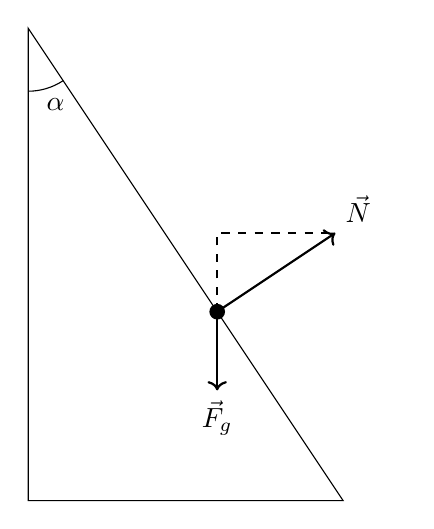
\begin{tikzpicture}
	    % Draw the triangle
	    \draw (0,0) -- (0,6) -- (4,0) -- cycle;

	    % Add the arc and label to the given angle
	    \draw (0,5.2) arc (-90:-56.31:0.8) coordinate (angle end);
	    \node [anchor=north west] at ($(0,5.2)!0.25!(angle end)$) {${\alpha}$};

	    % Pic an arbitrary point along the surface of the cone to represent
	    % the chain length element.
	    \coordinate (point) at ($(0,6)!0.6!(4,0)$);
	    \draw (point) node [fill,black,circle,inner sep=2pt] {};

	    % Draw the gravitational vector from the point
	    \draw [thick,->] (point) -- ++(0,-1)
		node [anchor=north] {$\vec F_g$};

	    % And the normal vector
	    \path [name path=Ny proj] ($(point)+(0,1)$) -- ($(point)+(2,1)$);
	    \path [name path=N vec] (point) -- ($(point)!1!90:(4,0)$);
	    \draw [name intersections={of=Ny proj and N vec, by=x}]
		[thick,->] (point) -- (x)
		node [anchor=south west] {$\vec N$}
		coordinate (norm end);

	    % Draw projections of the normal vector
	    \draw [thick,dashed] (point) -- ++(0,1) -- (norm end);
	\end{tikzpicture}
	\caption{Side View}
    \end{subfigure}
    \hfil
    \begin{subfigure}[b]{0.49\textwidth}
	\centering
	\begin{tikzpicture}
	    % Setup some coordinates:
	    \def\alpha{20}
	    \def\r{5cm}
	    \def\dr{0.2cm}
	    \def\Nr{1cm}
	    
	    \coordinate (center left)  at ($(90+\alpha:\r)$);
	    \coordinate (center mid)   at (90:\r);
	    \coordinate (center right) at ($(90-\alpha:\r)$);

	    \coordinate (outer left)   at ($(90+\alpha:\r+\dr)$);
	    \coordinate (outer mid)    at ($(90:\r+\dr)$);
	    \coordinate (outer right)  at ($(90-\alpha:\r+\dr)$);

	    \coordinate (inner left)   at ($(90+\alpha:\r-\dr)$);
	    \coordinate (inner mid)    at ($(90:\r-\dr)$);
	    \coordinate (inner right)  at ($(90-\alpha:\r-\dr)$);
	    
	    % Draw the radii
	    \draw [dashed] (0,0) -- (center left);
	    \draw [dashed] (0,0) -- (center mid);
	    \draw [dashed] (0,0) -- (center right);
	    % And label them
	    \node [anchor=west] at ($(0,0)!0.5!(center mid)$)   {$r$};
	    \node [anchor=west] at ($(0,0)!0.5!(center right)$) {$r$};

	    % Draw the chain
	    \draw [thick] (inner left) -- (outer left)
		arc (90+\alpha:90-\alpha:\r+\dr) -- (inner right)
		arc (90-\alpha:90+\alpha:\r-\dr);

	    % Draw the normal force
	    \draw (center mid) node [fill,black,circle,inner sep=2pt] {}
		node [anchor=west] {$ds$}
		[very thick,->] -- ++(0,\Nr)
		node [anchor=south] {$\vec N_r$};

	    % Finally, draw the tension vectors
	    \path [name path=Nr] ($(center mid)+(-4,-\Nr)$) -- ++(8,0);
	    \path [name path=Tl]
		(center left) -- ($(center left)!2.5cm!-90:(0,0)$);
	    \path [name path=Tr]
		(center right) -- ($(center right)!2.5cm!90:(0,0)$);

	    \draw [name intersections={of=Nr and Tl, by=x}]
		[very thick,->] (center left) -- (x)
		coordinate (left T end)
		node [anchor=north east] {$\vec T$};
	    \draw [name intersections={of=Nr and Tr, by=x}]
		[very thick,->] (center right) -- (x)
		coordinate (right T end)
		node [anchor=north west] {$\vec T$};
	    \draw [dashed] (left T end) -- (right T end);

	    % Add the known angles
	    \draw ($(0,0)!1cm!(center left)$) arc (90+\alpha:90-\alpha:1cm);
	    \node [anchor=south] at (0,1) {$d\phi $};
	    \draw ($(left T end)!1cm!(center left)$) arc ({\alpha}:0:1cm)
		node [anchor=north] {$\frac 12 d\phi $};
	\end{tikzpicture}
	\caption{Top View}
    \end{subfigure}
\end{figure}

Consider just a small element of the chain of arc length $ds$. It will have
a corresponding mass $dm = {\lambda}\,ds$ where ${\lambda} = m/L$. Knowing that it's a statics
problem, we can easily determine the normal force by balancing the vertical
component with that of gravity.
\begin{align*}
    F_g &= N \sin {\alpha} \\
    N &= \frac{{\lambda} g\,ds}{\sin {\alpha}}
\end{align*}
This leaves the horizontal component of the normal force to be balanced with
the tension within the chain.

Now switching to the top view, we consider the short chain segment $ds$, shown
above with an exagerated curvature. We note that the radial part of the
normal force must be opposed by the sum of the radial components of the two
tensions $T$ acting on the end of the chain segment. By geometry, we know that
the angle with respect to the midpoint's tangent is one half the differential
angle change $d\phi  = ds/r$. This means we balance the forces as
\begin{align*}
    2T\sin(\frac 12 d\phi ) &= N \cos {\alpha} \\
    2T\sin(\frac 12 d\phi ) &= {\lambda} g\,ds \cot {\alpha}
\end{align*}
By the small angle approximation, $\sin (\frac 12 d\phi ) \approx \frac 12 d\phi $, so after
substituting for the fact that $dr = L/2{\pi} $ and ${\lambda} = M/L$,
\begin{align}
    \boxed{
    T = \frac{Mg}{2{\pi} } \cot {\alpha}
    }
\end{align}

%%%%%%%%%%%%%%%%%%%%%%%%%%%%%%%%%%%%%%%%%%%%%%%%%%%%%%%%%%%%%%%%%%%%%%%%%%%%%%%
%%%% Problem 7
%%%%%%%%%%%%%%%%%%%%%%%%%%%%%%%%%%%%%%%%%%%%%%%%%%%%%%%%%%%%%%%%%%%%%%%%%%%%%%%
\problem{7}
\subsubsection{Question}
% Keywords
	\index{mechanics!Relativistic collision of electron and photon}

A laser beam (photon energy \SI{1}{\eV}) collides head-on with a \SI{50}{\GeV}
ultra-relativistic electron beam. What is the energy of the photons reflected
backwards in the collision?

\subsubsection{Answer}

We'll be solving the problem using conservation of 4-momentum, so we define
the following momenta with the assumption that the electron beam is moving
to the right, and the photons are initially moving to the left. Let the
unprimed and primed $q^{\mu}$ be the photon's 4-momentum before and after the
collision respectively, and define the electron's momenta $k^{\mu}$ similarly.
Then in terms of the energies $E$ and 3-momenta $p$ (actually taken to be 1D
without loss of generality) for each of the photon $\gamma $ and electron $e$:
\begin{align*}
    q^{\mu} &= \begin{pmatrix} E_\gamma /c \\ -E_\gamma /c \end{pmatrix} &
	q'^{\mu} &= \begin{pmatrix} E'_\gamma /c \\ E'_\gamma /c \end{pmatrix}
    \\
    k^{\mu} &= \begin{pmatrix} E_e/c \\ p_e \end{pmatrix} &
	k'^{\mu} &= \begin{pmatrix} E'_e/c \\ p'_e \end{pmatrix}    
\end{align*}
By conservation of momentum,
\begin{align*}
    q'^{\mu} + k'^{\mu} &= q^{\mu} + k^{\mu} \\
    k'^{\mu} &= q^{\mu} - q'^{\mu} + k^{\mu}
\end{align*}
Solving for the unknown electron momentum after the collision lets us eliminate
it from the equation; when we square the equation, the squared quantities are
Lorentz invariant, and therefore the product can be evaluated in any frame. A
convenient choice is the rest frame where the electron evaluates to its mass
energy and photons vanish.
\begin{align*}
    \underbrace{k'^{\mu} k'_{\mu}}_{m_e c^2} &=
	\underbrace{q^{\mu} q_{\mu}}_{0}
	- \underbrace{q'^{\mu} q'_{\mu}}_{0}
	+ \underbrace{k^{\mu} k_{\mu}}_{m_e c^2}
	- q'^{\mu} q_{\mu} + q'^{\mu} k_{\mu} - q^{\mu} k_{\mu}
\end{align*}
This greatly simplifies the rest of the problem to
\begin{align*}
    q'^{\mu} q_{\mu} - q'^{\mu} k_{\mu} &= - q^{\mu} k_{\mu}
\end{align*}
Inserting the energy and 3-momentum components and performing the inner
products,
\begin{align*}
    2\frac{E_\gamma  E'_\gamma }{c^2} - \frac{E'_\gamma  E_e}{c^2} + \frac{E'_\gamma  p_e}{c} &=
	-\frac{E_\gamma  E_e}{c^2} - \frac{E_\gamma  p_e}{c}
\end{align*}
Isolating $E'_\gamma $ on the left and $E_\gamma $ on the right,
\begin{align*}
    -E'_\gamma  (E_e - p_e c - 2E_\gamma ) &= - E_\gamma (E_e - p_e c)
\end{align*}
which solving for the unknown photon energy gives
\begin{align}
    \boxed{ E'_\gamma  = E_\gamma  (1 - \frac{2E_\gamma }{E_e - p_e c})^{-1} }
	\label{eqn:2002sp1.7:analytic_soln}
\end{align}

The solution is formally complete, but actually calculating a numerical answer
can prove difficult because $E_e \approx p_e c$. Therefore, we will expand the
solution. Beginning with the definition of the momentum from Einstein's energy
relation,
\begin{align*}
    p_e c &= \sqrt{{E_e}^2 - {m_e}^2c^4}
\intertext{we can subtract it from $E_e$, leading to the useful form}
    E_e - p_e c &= E_e ( 1 - \sqrt{1 - \frac{{m_e}^2c^4}{{E_e}^2}} )
\intertext{Expanding the root to first order in its argument,}
    E_e - p_e c &= E_e \cdot  \frac 12 \frac{{m_e}^2c^4}{{E_e}^2} \\
    {} &= \frac 12 \frac{{m_e}^2c^4}{E_e}
\end{align*}

Plugging this into the solution (\ref{eqn:2002sp1.7:analytic_soln}), the
photon energy is then approximately given by
\begin{align}
    \boxed{ E'_\gamma  \approx E_\gamma  ( 1 - 4 \frac{E_\gamma  E_e}{{m_e}^2c^4} )^{-1} }
	\label{eqn:2002sp1.7:approx_soln}
\end{align}
The numerics are much easier to calculate in this case, and we find that the
final energy of the reflected photon is
\begin{align}
    \boxed{ E'_\gamma  = \SI{4.273}{\eV} }
\end{align}

%%%%%%%%%%%%%%%%%%%%%%%%%%%%%%%%%%%%%%%%%%%%%%%%%%%%%%%%%%%%%%%%%%%%%%%%%%%%%%%
%%%% Problem 8
%%%%%%%%%%%%%%%%%%%%%%%%%%%%%%%%%%%%%%%%%%%%%%%%%%%%%%%%%%%%%%%%%%%%%%%%%%%%%%%
\problem{8}
\subsubsection{Question}
% Keywords
	\index{electrodynamics!LR circuit}

In the figure below, $\mathcal E = \SI{100}{\V}$, $R_1 = \SI{5}{\ohm}$,
$R_2 = \SI{10}{\ohm}$, $R_3 = \SI{15}{\ohm}$, and $L = \SI{1.0}{\henry}$. Find
the values of the currents $I_1$ and $I_2$
\begin{enumerate}[a)]
    \item immediately after the switch $S$ is closed,
    \item a long time later,
    \item immediately after switch $S$ is opened again,
    \item and then how long must you wait, after the switch is opened, before
	$I_2$ falls by a factor of $e$?
\end{enumerate}

\begin{center}
    \vspace{\baselineskip}
    \begin{circuitikz}
	\draw
	    (0,0)
		to[battery,l_=$\mathcal E$]
	    ++(0,3)
		to[closing switch,l_=$S$]
	    ++(3,0)
		to[resistor,l_=$R_1$]
	    ++(3,0)
		coordinate (I2 I3 break)
		to[resistor,l_=$R_3$,i=$I_3$]
	    ++(3,0)
		to[inductor,l_=$L$]
	    ++(0,-3)
		--
	    ++(-3,0)
		coordinate (I2 I3 combine)
		to[short,i=$I_1$]
	    (0,0)
	;
	\draw
	    (I2 I3 break)
		to[resistor,l_=$R_2$,i=$I_2$]
	    (I2 I3 combine)
	;
    \end{circuitikz}
    \vspace{\baselineskip}
\end{center}

\subsubsection{Answer}

Start by applying Kirchoff's rules to the circuit: current is conserved and
the voltage changes must sum to zero around each loop, so
\begin{align}
    I_1 &= I_2 + I_3
	\label{eqn:sp2002p1.8:kirchoff_current} \\
    0 &= \mathcal E - I_1R_1 - I_2R_2
	\label{eqn:sp2002p1.8:kirchoff_leftloop} \\
    0 &= -I_3R_3 - L \frac{dI_3}{dt} + I_2R_2
	\label{eqn:sp2002p1.8:kirchoff_rightloop}
\end{align}

Since only (\ref{eqn:sp2002p1.8:kirchoff_rightloop}) has a term involving
a time derivative, we choose to first solve for the current $I_3$. By solving
for $I_2R_2$ in (\ref{eqn:sp2002p1.8:kirchoff_leftloop}) and substituting,
we eliminate $I_2$ and have
\begin{align}
    0 &= -I_3R_3 - L\frac{dI_3}{dt} + \mathcal E - I_1R_1
    \label{eqn:sp2002p1.8:right_noI2}
\end{align}
Furthermore, by also substituting the value of $I_2$ into
(\ref{eqn:sp2002p1.8:kirchoff_current}):
\begin{align}
    I_1 &= \frac{\mathcal E}{R_1+R_2} + \frac{R_2}{R_1+R_2} I_3
    \label{eqn:sp2002p1.8:current_noI2}
\end{align}
Then by combining (\ref{eqn:sp2002p1.8:right_noI2}) and
(\ref{eqn:sp2002p1.8:current_noI2}), we can produce a differential equation
for $I_3$:
\begin{align*}
    -I_3R_3 - L\frac{dI_3}{dt} + \mathcal E - \frac{R_1}{R_1+R_2}\mathcal E -
	\frac{R_1R_2}{R_1+R_2}I_3 = 0
    \\
    -\underbrace{\frac{R_1R_2 + R_1R_3 + R_2R_3}{R_1+R_2}}_{R'}I_3 = L\frac{dI_3}{dt}
	- \frac{R_2}{R_1+R_2} \mathcal E
\end{align*}
\begin{align}
    \frac{dI_3}{dt} = -\frac{R'}{L} I_3 + \frac{1}{L}\frac{R_2}{R_1+R_2}\mathcal E
	\label{eqn:sp2002p1.8:diffeq_I3}
\end{align}
Considering just the homogeneous part, we easily solve it to find the standard
exponential solution
\begin{align*}
    I_{3h}(t) &= I_{30} e^{-R't/L}
\end{align*}
And using the ansatz $I_{3p}(t) = At + B$ for the inhomogeneous part,
\begin{align*}
    A &= -\frac{R'}{L}At - \frac{R'}{L}B + \frac 1L\frac{R_2}{R_1+R_2}\mathcal E
    \\
    A &= 0 \\
    B &= \frac{1}{R'}\frac{R_2}{R_1+R_2}\mathcal E
\end{align*}
At $t = 0$, the inductor has no current passing through it, so when the switch
is closed, the current must remain continuous. This gives us the initial
condition necessary to solve for the unknown $I_{30}$, and after doing so
and simplifying, the total solution is
\begin{align}
    I_3(t) &= \frac{\mathcal E}{R'}\frac{R_2}{R_1+R_2}(1 - e^{-R't/L})
	\label{eqn:sp2002p1.8:I3_charging}
\end{align}

Then by substituting this solution back into (\ref{eqn:sp2002p1.8:current_noI2})
we get the solution for $I_1$:
\begin{align}
    I_1(t) &= \frac{\mathcal E}{R_1+R_2} \left[ 1 + \frac{1}{R'}
	\frac{{R_2}^2}{R_1+R_2} (1 - e^{-R't/L}) \right]
	\label{eqn:sp2002p1.8:I1_charging}
\end{align}
Finally, combining both inserting both solutions for $I_1$ and $I_3$ into
(\ref{eqn:sp2002p1.8:kirchoff_current}), the solution for $I_2$ is
\begin{align}
    I_2(t) &= \frac{\mathcal E}{R_1+R_2} \left[ 1 - \frac{1}{R'}
	\frac{R_1R_2}{R_1+R_2} (1 - e^{-R't/L}) \right]
	\label{eqn:sp2002p1.8:I2_charging}
\end{align}

Plugging in all of the given values, we find that the currents at the instant
the switch is closed are
\begin{align}
    \boxed{I_1(0) = \SI{6.66}{\A}\quad\quad\text{$S$ is closed}} \\
    \boxed{I_2(0) = \SI{6.66}{\A}\quad\quad\text{$S$ is closed}}
\end{align}
For a long time later, we can let $t \rightarrow \infty $ and find that
\begin{align}
    \boxed{I_1(\infty ) = \SI{9.09}{\A}\quad\quad\text{$S$ is closed}} \\
    \boxed{I_2(\infty ) = \SI{5.54}{\A}\quad\quad\text{$S$ is closed}}
\end{align}

Right after the switch is opened, the left loop is taken out of the circuit,
so we immediately know that the value of $I_1$ is zero.
\begin{align}
    \boxed{I_1(0) = 0\quad\quad\text{$S$ is open	}}
\end{align}
For the right loop, we start by noting that the steady state current through
the inductor will be needed. Taking the limit of (\ref
{eqn:sp2002p1.8:I3_charging}), we have that the new initial condition is
\begin{align*}
    I_3(0) &= \frac{\mathcal E}{R'}\frac{R_2}{R_1+R_2}
\end{align*}
$I_2$ now is equal to $-I_3$ since there is no other path for the current to
traverse. This loop's differential equation is then
\begin{align*}
    -(R_2+R_3)I_3 - L\frac{dI_3}{dt} = 0
\end{align*}
Solving for the exponential and using the initial condition above, the time
solution is
\begin{align*}
    I_3(t) &= \frac{\mathcal E}{R'}\frac{R_2}{R_1+R_2} e^{-(R_2+R_3)t/L} \\
    I_2(t) &= -\frac{\mathcal E}{R'}\frac{R_2}{R_1+R_2} e^{-(R_2+R_3)t/L}    
\end{align*}
Therefore the current in $I_2$ just after the switch is opened reverses
direction
\begin{align}
    \boxed{I_2(0) = \SI{-3.64}{\A}}
\end{align}
Then by simple exponential relations, we know that the time time to decay by
a factor of $e$ is given by the reciprocal of the coefficient of $t$, so
inserting the appropriate numbers
\begin{align}
    \boxed{t_\mathrm{decay} = \SI{0.04}{\s}}
\end{align}

%%%%%%%%%%%%%%%%%%%%%%%%%%%%%%%%%%%%%%%%%%%%%%%%%%%%%%%%%%%%%%%%%%%%%%%%%%%%%%%
%%%% Problem 9
%%%%%%%%%%%%%%%%%%%%%%%%%%%%%%%%%%%%%%%%%%%%%%%%%%%%%%%%%%%%%%%%%%%%%%%%%%%%%%%
\problem{9}
\subsubsection{Question}
% Keywords
	\index{thermodynamics!Arbitrary engine efficiency}

An engine using \SI{1}{\mol} of an ideal diatomic gas performs the cycle $A
\rightarrow B \rightarrow C \rightarrow A$ as shown in the diagram below. $A
\rightarrow B$ is an adiabatic expansion, $B \rightarrow C$ occurs at
constant pressure, and $C \rightarrow A$ takes place at constant volume.
What is the efficiency of the cycle?

\begin{center}
    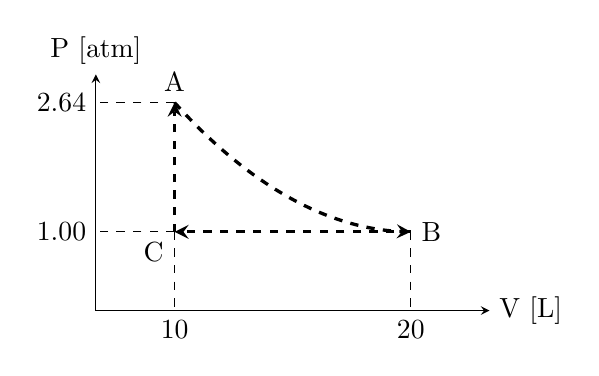
\begin{tikzpicture}[
	>=stealth
    ]
    % Draw the axes
	\draw [->] (0,0) -- (0,3) node [anchor=south] { P [\si{atm}] };
	\draw [->] (0,0) -- (5,0) node [anchor=west] {V [\si{\L}]};

	% Then draw the engine cycle
	\draw [very thick,dashed,->] (1,1)    -- (1, 2.64)
	    node [anchor=south] {A};
	\draw [very thick,dashed,->] (1,2.64) parabola[bend at end] (4,1)
	    node [anchor=west] {B};
	\draw [very thick,dashed,->] (4,1)    -- (1,1)
	    node [anchor=north east] {C};
	;

	% Then draw in the labels that give the absolute numbers
	\draw [dashed] (1,2.64) -- (0,2.64) node [anchor=east] {2.64};
	\draw [dashed] (1,1) -- (0,1) node [anchor=east] {1.00};
	\draw [dashed] (1,1) -- (1,0) node [anchor=north] {10};
	\draw [dashed] (4,1) -- (4,0) node [anchor=north] {20};
    \end{tikzpicture}
\end{center}

\subsubsection{Answer}

Since we want to find the efficiency of the cycle, we only care about the
heat exchanged during each stage of the cycle. Because the path $A
\rightarrow B$ is adiabatic, we immediately know that $Q = 0$. Then
proceeding to look at the stage $C \rightarrow A$, we know that the work
done during this cycle is identically zero since there is no area under the
curve. That means we are left simply with the equation
\begin{align*}
    dU = dQ
\end{align*}
Because this is an ideal [diatomic] classical gas, we combine the equations
\begin{align*}
    U &= \frac 52 nRT
\intertext{and}
    PV &= nRT
\end{align*}
to get that the difference in energy across the path is
\begin{align*}
    Q_{CA} &= U = \frac 52 nR(T_A - T_C) \\
    {}&= \frac 52 V_1 (P_2 - P_1)
\end{align*}

For the remaining stage $B \rightarrow C$, we use the full thermodynamic
identity:
\begin{align*}
    dU &= dQ - P\,dV
\end{align*}
The pressure $P_1$ is constant, so both integration of $dU$ and $dV$ are simply
the differences in each quantity. Again substituting for the temperature in
$U$ with the ideal gas law,
\begin{align*}
    \frac 52 nR(T_C - T_B) &= Q_{BC} - P_1(V_1 - V_2) \\
    \frac 52 P_1(V_1 - 2V_1) &= Q_{BC} + P(V_1 - 2V_1) \\
    Q_{BC} &= -\frac 72 P_1V_1
\end{align*}

We've accounted for all the heat flow in the system. $Q_{BC}$ is negative, so
this is the heat flow out of the system, while $Q_{CA}$ is positive and is the
heat flow into the system. By definition then, the efficiency ${\eta}$ of the system
is
\begin{align*}
    {\eta} &= 1 - \frac{Q_{out}}{Q_{in}} \\
    {}&= 1 - \frac{\frac 72 P_1 V_1}{\frac 52 V_1 (P_2 - P_1)} \\
    {}&= 1 - \frac 57 \frac{P_1}{P_2 - P_1}
\end{align*}
Plugging in the given values, we find the efficiency to be
\begin{align}
    \boxed{
    {\eta} = 0.146 = \SI{14.6}{\percent}
    }
\end{align}

%%%%%%%%%%%%%%%%%%%%%%%%%%%%%%%%%%%%%%%%%%%%%%%%%%%%%%%%%%%%%%%%%%%%%%%%%%%%%%%
%%%% Problem 10
%%%%%%%%%%%%%%%%%%%%%%%%%%%%%%%%%%%%%%%%%%%%%%%%%%%%%%%%%%%%%%%%%%%%%%%%%%%%%%%
\problem{10}
\subsubsection{Question}
% Keywords
	\index{mechanics!Friction and a rolling hoop}

A thin circular hoop rolls down an inclined plane under the influence of
gravity. What minimum coefficient of friction is required to ensure that it
rolls rather than slides?

\subsubsection{Answer}

Begin first by finding the motion that describes the rolling without slipping
state. We do this by solving the system's Lagrangian:
\begin{align*}
    \mathcal L &= (\frac 12 m{\dot x}^2 + \frac 12 I{\dot \theta }^2) - (mgx\sin {\alpha})
\end{align*}
where $x$ is the length along the ramp with $x=0$ at the bottom, $I$ is the
moment of inertia of the hoop, $m$ is its mass, $\theta $ is the angle of rotation
of the hoop about its center, and ${\alpha}$ is the angle of the incline plane. By
noting that rolling without slipping requires that $r\dot \theta  = \dot x$, we
can reduce the problem to the single variable $x$. The result is the following
differential equation, where $I = mR^2$ has been substituted in:
\begin{align*}
    2m \ddot x &= -mg\sin {\alpha} \\
    \ddot x &= -\frac 12 g\sin {\alpha}
\end{align*}
Therefore we know the linear acceleration will be $a = -\frac 12 g\sin {\alpha}$ in
the non-slipping case.

To find what coefficient of friction produces this motion, we consider the
forces acting on the hoop with the coordinate system still oriented along and
perpendicular to the plane. In the perpendicular direction, the normal force
$N$ is canceled by the perpendicular component of gravity, so
\begin{align*}
    N &= mg\cos {\alpha}
\end{align*}
In the parallel direction, the frictional force and the parallel component of
gravity must sum to give the requisite force, namely $ma$.
\begin{align*}
    {\mu}N - mg\sin {\alpha} &= ma = -\frac 12 mg\sin {\alpha} \\
    {\mu}mg\cos {\alpha} &= \frac 12 mg\sin {\alpha} \\
    {\mu} &= \frac 12 \tan {\alpha}
\end{align*}

\fbox{
Therefore we find that the coefficient of friction must be equal to half of
the tangent of the inclined plane's angle.
}

%%%%%%%%%%%%%%%%%%%%%%%%%%%%%%%%%%%%%%%%%%%%%%%%%%%%%%%%%%%%%%%%%%%%%%%%%%%%%%%
%%%% Problem 11
%%%%%%%%%%%%%%%%%%%%%%%%%%%%%%%%%%%%%%%%%%%%%%%%%%%%%%%%%%%%%%%%%%%%%%%%%%%%%%%
\problem{11}
\subsubsection{Question}
% Keywords
	\index{quantum!Probability to stay in ground state}

A particle is confined within a cubical box with sides of length $L$ and is
initially in the ground state. If the length of one side of the box (along
the $x$-direction) is abruptly increased to a length $2L$, what is the
probability that the particle remains in the ground state?

\subsubsection{Answer}

We start by recalling the solution for a particle in a box. In a 1D box with is
left edge at the origin, the properly normalized wavefunction is given by
\begin{align*}
    \psi (x) &= \sqrt{\frac{2}{L}} \sin (\frac{n{\pi} x}{L})
\end{align*}
where $L$ is the size of the box. The Cartesian extension into 3D is simple
and is respectively for the $L\times L\times L$ and $2L\times L\times L$ boxes:
\begin{align*}
    \psi (x,y,z) &= (\frac{2}{L})^{3/2} \sin(\frac{n_x {\pi} x}{L})
	\sin(\frac{n_y {\pi} y}{L}) \sin(\frac{n_y {\pi} y}{L}) \\
    \psi '(x,y,z) &= \frac{1}{\sqrt 2}(\frac{2}{L})^{3/2} \sin(\frac{n_x {\pi} x}{2L})
	\sin(\frac{n_y {\pi} y}{L}) \sin(\frac{n_y {\pi} y}{L})
\end{align*}

To find the probability of remaining in the ground state, we simply must
take the inner product of both wavefunctions in the ground state over an
appropriate domain; this means that the initial, unexanded box's wavefunction
is 0 within the new region.
\begin{align*}
    \mathscr{P} &= \braket{\psi _{111}}{\psi '_{111}} \\
    {} &= \frac{1}{\sqrt{2}} (\frac{2}{L})^3  (\int_0^L \sin(\frac{{\pi} x}{L})
	\sin(\frac{{\pi} x}{2L}) \,dx) (\int_0^L \sin(\frac{{\pi} y}{L})
	\sin(\frac{{\pi} y}{L}) \,dy) (\int_0^L \sin(\frac{{\pi} z}{L})
	\sin(\frac{{\pi} z}{L}))
\end{align*}
The integrals over $y$ and $z$ are simple and simply evaluate to $L/2$ as
we'd expect from the normalization factor. To evaluate the integral over $x$,
use the trigonometric identity $\sin 2\theta  = 2\sin \theta  \cos \theta $ and a change of
variables with $u = \sin({\pi} x/2L)$ to arrive at the integral
\begin{align*}
    \mathscr{P} &= \frac{2\sqrt 2}{L} \int_0^1 u^2 \cdot  \frac{2L}{{\pi} }\,du
\end{align*}
Evaluating this, we find the probability of remaining the ground state after
the box is expanded suddenly to be
\begin{align}
    \boxed{\mathscr{P} = \frac{4\sqrt 2}{3{\pi} } \approx 0.60}
\end{align}

%%%%%%%%%%%%%%%%%%%%%%%%%%%%%%%%%%%%%%%%%%%%%%%%%%%%%%%%%%%%%%%%%%%%%%%%%%%%%%%
%%%% Problem 12
%%%%%%%%%%%%%%%%%%%%%%%%%%%%%%%%%%%%%%%%%%%%%%%%%%%%%%%%%%%%%%%%%%%%%%%%%%%%%%%
\problem{12}
\subsubsection{Question}
% Keywords
	\index{mechanics!Deep-water gravity waves}
	\index{waves!Deep-water gravity waves}

The frequency $f$ of a deep water gravity wave (i.e. an ordinary ocean wave)
is given by
\begin{align*}
    f =\sqrt{\frac{1}{2{\pi} }} \rho ^a g^b {\lambda}^c
\end{align*}
where $\rho $, $g$, and ${\lambda}$ are the water density, gravitational acceleration, and
wavelength of the wave, respectively. What are the values of the exponents
$a$, $b$, and $c$, and what is the ratio of the wave group velocity to phase
velocity?

\subsubsection{Answer}

We proceed by dimensional analysis. Immediately we know that $a = 0$ since a
frequency does not have a mass component, and neither $g$ nor ${\lambda}$ have a
mass term to cancel the one in $\rho $. Furthermore, $g$ is the only one with a
time term, so it's exponent must then by $b = \frac 12$ in order to give $f$
its $[\si{\s^{-1}}]$ unit. That leaves $c = \frac 12$ in order to cancel
the $\sqrt{\si{\m}}$ dimension left over from $g$.

\begin{align*}
    \boxed{
    f = \sqrt{\frac{g{\lambda}}{2{\pi} }}
	\quad\quad\text{ with }\quad a = 0,\, b = \frac 12,\, c = \frac 12
    }
\end{align*}

The phase velocity can be derived from the frequency given by noting that
$v_p = {\omega} /k$ together with $k^{-1} = 2{\pi} {\lambda}$ and ${\omega}  = 2{\pi} f$. Put together, this
gives
\begin{align*}
    v_p &= \frac{1}{k}\sqrt{\frac{g}{k}}
\end{align*}
The group velocity is given by $v_g = d{\omega} /dk$, so
\begin{align*}
    v_g &= -\frac{1}{2k}\sqrt{\frac{g}{k}}
\end{align*}
Taking only the absolute values and finding the ratio
\begin{align}
    \boxed{\frac{v_g}{v_p} = \frac 12}
\end{align}


\springexam{2002}{2}
%%%%%%%%%%%%%%%%%%%%%%%%%%%%%%%%%%%%%%%%%%%%%%%%%%%%%%%%%%%%%%%%%%%%%%%%%%%%%%%
%%%% Problem 2
%%%%%%%%%%%%%%%%%%%%%%%%%%%%%%%%%%%%%%%%%%%%%%%%%%%%%%%%%%%%%%%%%%%%%%%%%%%%%%%
\problem{2}
\subsubsection{Question}
% Keywords
	\index{thermodynamics!Zipper partition function}
    \index{statistical mechanics!Zipper partition function}

A zipper has $N$ links; each link has a closed state with zero energy and an
open state with energy $\varepsilon $. We require, however, that the zipper can only
unzip from the left end, and that the link number $s$ can only open if all
links to the left (i.e.\ $1, 2, \ldots s-1$) are already open.
\begin{enumerate}[a.]
    \item
        Find an explicit expression for the partition function by doing the
        appropriate summation.
    \item
        In the limit $\varepsilon \gg k_B T$ find the average number of open links. This
        model is a very simplified model of the unwinding of two-stranded
        DNA molecules.
\end{enumerate}

\subsubsection{Answer}

\begin{enumerate}[a.]
    \item
        Create the partition function by induction; start by assuming there is
        only a single link. Then the partition function is a simple two-state
        system:
        \begin{align*}
            Z_1 &= e^0 + e^{-\varepsilon /k_BT} = 1 + e^{-\varepsilon /k_BT}
        \end{align*}
        Adding a second link,
        \begin{align*}
            Z_2 &= \underbrace{e^{0+0}}_{\text{both closed}} +
                \underbrace{e^{(-\varepsilon +0)/k_BT}}_{\text{1 open, 1 closed}} +
                \underbrace{e^{(-\varepsilon -\varepsilon )/k_BT}}_{\text{both open}}
            \\
            {} &= 1 + e^{-\varepsilon /k_BT} + e^{-2\varepsilon /k_BT}
        \end{align*}
        Following, for three links:
        \begin{align*}
            Z_3 &= \underbrace{e^{0+0+0}}_{\text{all closed}} +
                \underbrace{e^{(-\varepsilon +0+0)/k_BT}}_{\text{1 open, 2 closed}} +
                \underbrace{e^{(-\varepsilon -\varepsilon +0)/k_BT}}_{\text{2 open, 1 closed}} +
                \underbrace{e^{(-\varepsilon -\varepsilon -\varepsilon )/k_BT}}_{\text{all open}}
            \\
            {} &= 1 + e^{-\varepsilon /k_BT} + e^{-2\varepsilon /k_BT} + e^{-3\varepsilon /k_BT}
        \end{align*}
        By induction, we see that the maximum coefficient in the series of
        exponential factors is just the number of links, so by induction we
        conclude that
        \begin{align*}
            Z &= \sum_{s=0}^{N} e^{-s\varepsilon /k_BT}
        \end{align*}
        Applying the results of a finite geometric series, the closed-form
        solution for the partition function of the links is
        \begin{align}
            \boxed{
            Z = \frac{1 - e^{-(N+1)\varepsilon /k_BT}}{1 - e^{-\varepsilon /k_BT}}
            }
        \end{align}
    \item
        To get the average number of open links, we use the standard
        procedure for finding expvalation values.
        \begin{align*}
            \expval{s} &= \frac{1}{Z} \sum_{s=0}^N s e^{-s\varepsilon /k_BT}
        \end{align*}
        By making use of differentiation under the summation trick, we can
        find the closed-form solution:
        \begin{align*}
            \expval{s} &= \frac{1}{Z} \sum_{s=0}^N
                \frac{d}{d(\frac{\varepsilon }{k_BT})} \Big[ -e^{-s\varepsilon /k_BT} \Big] \\
            {} &= -\frac{1}{Z} \frac{\partial }{\partial (\frac{\varepsilon }{k_BT})}
                \sum_{s=0}^N e^{-s\varepsilon /k_BT} \\
        \intertext{
        Noting that the summation is the same as above,
        }
            \expval{s} &= -\frac{1}{Z} \frac{\partial Z}{\partial (\frac{\varepsilon }{k_BT})}
        \end{align*}
        First considering just the derivative part:
        \begin{align*}
            \frac{\partial Z}{\partial (\frac{\varepsilon }{k_BT})} &=
                \frac{(N+1)e^{-(N+1)\varepsilon /k_BT}}{1 - e^{-\varepsilon /k_BT}} -
                \frac{1 - e^{-(N+1)\varepsilon /k_BT}}{(1 - e^{-\varepsilon /k_BT})^2} e^{-\varepsilon /k_BT}
        \intertext{
        which when combined with the factor $-1/Z$ simplifies to
        }
            -\frac{1}{Z} \frac{\partial Z}{\partial (\frac{\varepsilon }{k_BT})} &=
                -(N+1)\frac{e^{-(N+1)\varepsilon /k_BT}}{1 - e^{-(N+1)\varepsilon /k_BT}} +
                \frac{e^{-\varepsilon /k_BT}}{1 - e^{-\varepsilon /k_BT}} \\
            &= \frac{1}{e^{\varepsilon /k_BT} - 1} - \frac{N+1}{e^{(N+1)\varepsilon /k_BT} - 1}
        \end{align*}
        Therefore the analytic solution is
        \begin{align}
            \boxed{
            \expval{s} = \frac{1}{e^{\varepsilon /k_BT}-1} - \frac{N+1}{e^{(N+1)\varepsilon /k_BT}-1}
            }
        \end{align}
        In the limit that $\varepsilon \gg k_BT$, though, the exponentials in the denominator
        are very large in comparison to 1, so we ignore the unity factors
        and make the approximation that
        \begin{align*}
            \expval{s} &= e^{-\varepsilon /k_BT} - (N+1)e^{-(N+1)\varepsilon /k_BT}
        \intertext{
        Collecting like terms,
        }
            {} &= \left[1 - (N+1)e^{-N\varepsilon /k_BT} \right] e^{-\varepsilon /k_BT}
        \intertext{
            The second term in the brackets approximate zero, so
        }
            {} &= e^{-\varepsilon /k_BT}
        \end{align*}
        Therefore in the low temperature limit where the thermal energy is
        much less than the energy of the open state,
        \begin{align}
            \boxed{
            \expval{s} = e^{-\varepsilon /k_BT}
            }
        \end{align}
\end{enumerate}


\fallexam{2002}{1}
%%%%%%%%%%%%%%%%%%%%%%%%%%%%%%%%%%%%%%%%%%%%%%%%%%%%%%%%%%%%%%%%%%%%%%%%%%%%%%%
%%%% Problem 5
%%%%%%%%%%%%%%%%%%%%%%%%%%%%%%%%%%%%%%%%%%%%%%%%%%%%%%%%%%%%%%%%%%%%%%%%%%%%%%%
\problem{5}
\subsubsection{Question}
% Keywords
	\index{mechanics!Elastic collision on spring-connected blocks}
	\index{Lagrangian!Elastic collision on spring-connected blocks}

Blocks of mass $m$ and $2m$ are free to slide without friction on a
horizontal wire. They are connected by a massless spring of equilibrium
length $L$ and force constant $k$. A projectile of mass $m$ is fired with
velocity $v$ into the block with mass $m$ and sticks to it. If the blocks
are initially at rest, what is the maximum displacement between them in the
subsequent motion?

\subsubsection{Answer}

Take time $t=0$ to be the moment the projectile collides with the mass $m$,
and let the subsequent transfer of momentum be instantaneous. In this case,
the initial conditions of the problem are then:
\begin{align*}
    x₁(0) &= 0			& \dot x₁(0) &= u \\
    x₂(0) &= L			& \dot x₂(0) &= 0
\end{align*}
where $u$ is the initial velocity of the combined project-mass system. We get
$u$ from conservation of mometum:
\begin{align*}
    2mu &= mv + 0 \\
    u &= \frac 12 v
\end{align*}

Now solve the mechanics problem using the Lagrangian approach. Both masses have
kinetic energy, and the spring stores potential energy, so
\begin{align*}
    T &= m{\dot x₁}² + m{\dot x₂}² \\
    V &= \frac 12 m (x₂ - x₁)² \\
    L &= m ({\dot x₁}² + {\dot x₂}²) - \frac 12 k({x₁}² + {x₂}² + 2x₁x₂)
\end{align*}
Setting up the differential equation, we get
\begin{align*}
    \frac{∂L}{∂x₁} &= -kx₁ + kx₂	& \frac{d}{dt}
	\left[\frac{∂L}{∂\dot x₁}\right] &= 2m \ddot x₁ \\
    \frac{∂L}{∂x₂} &=  kx₁ - kx₂	& \frac{d}{dt}
	\left[\frac{∂L}{∂\dot x₁}\right] &= 2m \ddot x₂ \\
\end{align*}
Leading to the system of equations where $ω² = k/2m$,
\begin{align*}
    \begin{bmatrix} \ddot x₁ \\ \ddot x₂ \end{bmatrix} &=
	\begin{bmatrix} -ω² & ω² \\ ω² & -ω² \end{bmatrix}
	\begin{bmatrix} x₁ \\ x₂ \end{bmatrix}
\end{align*}
Solving the eigensystem, we find the eigenfrequencies to be $λ = \{0, -2ω²\}$.
Letting ${ω'}² = 2ω²$, the eigenfunction equations are then
\begin{align*}
    \ddot ψ₁ &= 0
	& \rightarrow&&
	ψ₁ &= A₁t + B₁ \\
    \ddot ψ₂ &= -2ω² ψ₂
	& \rightarrow&&
	ψ₂ &= A₂\cos(ω't) + B₂\sin(ω't)
\end{align*}
From the eigenvectors, we express the solutions of $x₁$ and $x₂$ in terms of
$ψ₁$ and $ψ₂$:
\begin{align*}
    \begin{bmatrix} x₁ \\ x₂ \end{bmatrix} &=
	\begin{bmatrix} 1 & 1 \\ 1 & -1 \end{bmatrix}
	\begin{bmatrix} ψ₁ \\ ψ₂ \end{bmatrix}
\end{align*}
\begin{align*}
    x₁ &= A₁t + B₁ + A₂\cos(ω't) + B₂\sin(ω't) \\
    x₂ &= A₁t + B₁ - A₂\cos(ω't) - B₂\sin(ω't)
\end{align*}
Applying the boundary conditions, we find that
\begin{align*}
    x₁(t) &= \frac 14 vt + \frac 12 L - \frac 12 L\cos(ω't) +
	\frac{v}{4ω'}\sin(ω't) \\
    x₂(t) &= \frac 14 vt + \frac 12 L + \frac 12 L\cos(ω't) -
	\frac{v}{4ω'}\sin(ω't)
\end{align*}
The distance $ℓ(t) = x₂(t) - x₁(t)$ between the two masses maximizes when
\begin{align*}
    \frac{dℓ}{dt} = 0 &= \frac{d}{dt} \left[ L\cos(ω't) -
	\frac{v}{2ω'}\sin(ω't) \right] \\
    t &= -\frac{1}{ω'} \arctan (\frac{v}{2Lω'})
\end{align*}
Plugging back into the function $ℓ(t)$,
\begin{align*}
    ℓ &= L\cos \left[ -\arctan (\frac{v}{2Lω'}) \right] - \frac{v}{2ω'}
	\sin \left[ -\arctan (\frac{v}{2Lω'}) \right] \\
    ℓ &= L \frac{2Lω'}{\sqrt{v² + 4L² {ω'}²}} + \frac{v}{2ω'}
	\frac{v}{\sqrt{v² + 4L² {ω'}²}} \\
    ℓ &= \frac{\sqrt{v² + 4L² {ω'}²}}{2ω'}
\end{align*}
Finally, substituting back in $ω' = \sqrt{2k/m}$ and simplifying, we get the
final solution that maximum distance between the two masses is
\begin{empheq}[box=\fbox]{align}
    ℓ &= \sqrt{L² + \frac{\frac 12 mv²}{8k}}
\end{empheq}
which agrees qualitatively with the fact that a larger spring constant should
stiffen the system and decrease the maximum displacement, while launching the
projectile with a greater velocity would increase it.

%%%%%%%%%%%%%%%%%%%%%%%%%%%%%%%%%%%%%%%%%%%%%%%%%%%%%%%%%%%%%%%%%%%%%%%%%%%%%%%
%%%% Problem 10
%%%%%%%%%%%%%%%%%%%%%%%%%%%%%%%%%%%%%%%%%%%%%%%%%%%%%%%%%%%%%%%%%%%%%%%%%%%%%%%
\problem{10}
\subsubsection{Question}
% Keywords
	\index{dimensional analysis!Freezing ice}
	\index{thermodynamics!Freezing ice}

Ice on a pond is \SI{10}{\cm} thick and the water temperature just below the
ice is \SI{0}{\celsius}. If the air temperature is \SI{-20}{\celsius}, by
how much will the ice thickness increase in 1 hour? Assuming that the air
temperature stays the same over a long period, how will the ice thickness
increase with time? Comment on any approximation that you make in your
calculation.

Density of ice ${}= \SI{0.9}{\g\per\cm\cubed}$

Thermal conductivity of ice ${}= \SI{0.0005}{\cal\per\cm\per\s\per\celsius}$

Latent heat of fusion of water ${}= \SI{80}{\cal\per\g}$

\subsubsection{Answer}

Since the thermal heat flow is a one dimensional problem, immediately
consider everything with respect to a small area element with its normal
perpendicular to the ice-water interface $dA$. Then we want to know how much
ice is generated on the surface of the ice. This small ice element's mass is
simply
\begin{align*}
    dm &= ρ\,dA\,dz
\end{align*}
where $dz$ is the thickness of the new ice layer. To generate this ice, the
latent heat of fusion must be conducted away, so the energy released is,
\begin{align*}
    dE_f &= L_f\,dm \\
    {} &= L_f ρ \,dA\,dz
\end{align*}

The energy flow is through the ice, and we expect this to increase with the
temperature differential across the ice sheet, suggesting that the thermal
conductivity $κ$ be multiplied by the temperature difference $ΔT$. Furthermore,
the ice will decrease the rate of heat flow as it becomes thicker, so the
quantity should also be divided by the thickness $z$. This gives
\begin{align*}
    \frac{κ ΔT}{z} &= \left[ \si{\cal\per\cm\squared\per\s}
	\right]
\end{align*}
This energy is flowing through a surface element $dA$, giving the power flow
due to heat as
\begin{align*}
    \frac{κΔT\,dA}{z} &= \left[ \si{\cal\per\s} \right]
\end{align*}

This power can be matched in units with the energy released from the ice
calculated above by taking the time derivative of $dE_f$, so equating the two
we have
\begin{align*}
    L_f ρ \,dA\frac{dz}{dt} &= \frac{κΔT\,dA}{z} \\
    ∫_{z₀}^{z₀+δz} z\,dz &= ∫_0^t \frac{κΔT}{L_f ρ}\,dt \\
    2z₀ δz + (δz)² &= \frac{κΔT}{L_f ρ}t
\end{align*}
Solving for the length the ice grows $δz$,
\begin{align*}
    δz &= \frac{-2z₀ ± \sqrt{4{z₀}² - 4(\frac{κΔT}{L_f ρ})t} }{2} \\
    δz &= z₀(1 ± \sqrt{1 - \frac{κΔT}{L_f ρ {z₀}²} t})
\end{align*}
The two roots give solutions $δz = \{ \SI{0.0501}{\cm}, \SI{19.950}{\cm} \}$.
Since the second root is unrealistic, we know that the solution must then be
\begin{empheq}[box=\fbox]{align}
    δz &= \SI{0.0501}{\cm} \quad\text{in an hour}
\end{empheq}

%%%%%%%%%%%%%%%%%%%%%%%%%%%%%%%%%%%%%%%%%%%%%%%%%%%%%%%%%%%%%%%%%%%%%%%%%%%%%%%
%%%% Problem 11
%%%%%%%%%%%%%%%%%%%%%%%%%%%%%%%%%%%%%%%%%%%%%%%%%%%%%%%%%%%%%%%%%%%%%%%%%%%%%%%
\problem{11}
\subsubsection{Question}
% Keywords
	\index{statistical mechanics!Carbon-14 dating}

Carbon-14 is produced by cosmic rays interacting with the nitrogen in the
Earth's atmosphere. It is eventaully incorporated into all living things,
and since it has a half-life of \SI{5730(40)}{\year}, it is useful for
dating archaeological specimens up to several tens of thousands of years
old. The radioactivity of a particular specimen of wood containing \SI{3}{\g}
of carbon was measured with a counter whose efficiency was
\SI{18}{\percent}; a count rate of \SI{12.8(1)}{\minute^{-1}} was measured.
It is known that in \SI{1}{\g} of living wood, there are
\SI{16.1}{\minute^{-1}} radioactive carbon-14 decays. What is the age of
this specimen, and its uncertainity? (Where errors are not quoted, they can
be assumed to be negligible).

\subsubsection{Answer}
The rate $N$ after a given time is given by the exponential decay formula
\begin{align*}
    N(t) &+= N₀ e^{-t/τ}
\end{align*}
Since we have the half-life $t_{1/2}$ instead of the decay constant $τ$, we
use the relation $t_{1/2} = τ\ln 2$ to simplify the expression instead to
\begin{align*}
    N(t) &= N₀ (\frac 12)^{t/t_{1/2}}
\end{align*}

The counter use has an efficiency of $ε = 0.18$, so the measured counting
rate $N_m$ must be corrected for that. Furthermore, the sample has a mass of
\SI{3}{\g} whereas we know the rate for a one gram sample, so we also
normalize the count rate by the mass of the sample. Plugging this all into
the exponential decay function above gives
\begin{align*}
    \frac{N_m}{3ε} &= N₀ (\frac 12)^{t/t_{1/2}}
\end{align*}
The only unknown left in the equation is the time, so solving for it,
\begin{align*}
    t &= t_{1/2} \log_{1/2} (\frac{N_m}{3εN₀}) \\
    t &= t_{1/2} \frac{\ln (\frac{N_m}{3εN₀})}{\ln 2} \\
    t &= \frac{t_{1/2}}{\ln 2} \ln (\frac{N_m}{3εN₀})
\end{align*}

To find the uncertainty, we note that only the quantities $N_m$ and $t_{1/2}$
have non-negligible uncertainties, so we propagate the errors only over
these two terms:
\begin{align*}
    {σ_t}² &= (-\frac{t_{1/2}}{N_m \ln 2})² {σ_{N_m}}² +
	(\frac{1}{\ln 2} \ln(\frac{3εN₀}{N_m}))² {σ_{t_{1/2}}}² \\
    σ_t &= \frac{t_{1/2}}{\ln 2} \sqrt{ (\frac{σ_{N_m}}{N_m})² +
	(\frac{σ_{t_{1/2}}}{t_{1/2}})² \left[ \ln(\frac{3εN₀}{N_m}) \right]²}
\end{align*}
Plugging in all the numbers, we get $t = \SI{4248.8435}{\year}$ and $σ_t =
\SI{161.717}{\year}$. The given uncertainties have a single significant digit,
so adding an extra significant figure to the uncertainity and matching decimal
places in the answer, we conclude that the sample has an age of
\begin{empheq}[box=\fbox]{align}
    t &= \SI{4250(160)}{\year}
\end{empheq}


\fallexam{2007}{1}
%%%%%%%%%%%%%%%%%%%%%%%%%%%%%%%%%%%%%%%%%%%%%%%%%%%%%%%%%%%%%%%%%%%%%%%%%%%%%%%
%%%% Problem 9
%%%%%%%%%%%%%%%%%%%%%%%%%%%%%%%%%%%%%%%%%%%%%%%%%%%%%%%%%%%%%%%%%%%%%%%%%%%%%%%
\problem{9}
\subsubsection{Question}
% Keywords
	\index{thermodynamics!Light bulb as blackbody radiator}
	\index{circuits!Light bulb as blackbody radiator}

An electric bulb is rated at \SI{100}{\W} when used with a DC voltage of \SI
{110}{\V}. What total power is dissipated if this voltage is applied to two
such bulbs connected in series? It can be assumed that each bulb dissipates
heat by radiation from its filament similar to a black body and that the
resistance of the filament is proportional to its absolute temperature.

\subsubsection{Answer}

Beginning from the known properties of a single bulb, we know that the
dissipated power in a single bulb $P_0$ is like a black body, so the power
must follow the Stefan-Boltzmann law:
\begin{align*}
	P_0 &= {\sigma}_B {T_0}^4
\end{align*}
where $T_0$ is operating equilibrium temperature. In addition, we are told
that the bulb is like a resistor with a resistance proportional to its
temperature:
\begin{align*}
	P_0 &= \frac{V^2}{R} = \frac{V_0^2}{C T_0}
\end{align*}
Combining the two equations gives the proportionality constant for a single
bulb in the circuit.
\begin{align*}
	C &= \frac{{V_0}^2}{{\sigma}_B {T_0}^5}
\end{align*}

When a second bulb is added to the circuit, the voltage across each bulb is
dropped and a corresponding change in the equilibrium temperature is
created. Since the bulbs are in series, the voltage $V = \frac 12 V_0$ across
each resistor sums in series. Repeating the same procedure as in the first
case,
\begin{align*}
	{\sigma}_B T^4 &= 2 \frac{V^2}{R} = 2 \frac{(\frac 12 V_0)^2}{C T} \\
	{\sigma}_B T^5 &= \frac 12 \frac{{V_0}^2}{C}
\end{align*}
and inserting the constant $C$,
\begin{align*}
	T^5 &= \frac 18 {T_0}^5 \\
	T &= \frac{1}{2^{1/5}} T_0
\end{align*}
Therefore from the Stefan-Boltmann law, the total power dissipated is
\begin{align*}
	P &= {\sigma}_B T^4 = \frac{1}{2^{4/5}} {\sigma}_B {T_0}^4
\end{align*}
\begin{align}
	\boxed{ P = \frac{\SI{100}{\W}}{2^{4/5}} = \SI{57.435}{\W} }
\end{align}



\fallexam{2008}{1}
%%%%%%%%%%%%%%%%%%%%%%%%%%%%%%%%%%%%%%%%%%%%%%%%%%%%%%%%%%%%%%%%%%%%%%%%%%%%%%%
%%%% Problem 2
%%%%%%%%%%%%%%%%%%%%%%%%%%%%%%%%%%%%%%%%%%%%%%%%%%%%%%%%%%%%%%%%%%%%%%%%%%%%%%%
\problem{2}
\subsubsection{Question}
% Keywords
	\index{mechanics!Impulse on a rod}

If an impulse is delivered to the end of a uniform rod of length $ℓ$, lying on
a frictionless plane, how far will it travel while making one revolution? The
impulse is in the plane of the table and perpendicular to the rod.

\subsubsection{Answer}

For a given impulse $\vec J$, the change in the motion is $\vec J = Δ\vec p$.
If the rod start at rest, then the final momentum must be $\vec p = \vec J$.
This means the rod is moving laterally with a velocity
\begin{align*}
    V = \frac 1m \vec J
\end{align*}
which when integrated over a time $t$ gives the distance it has moved $\vec x$.
\begin{align*}
    \vec x = \frac 1m \vec J t
\end{align*}

The impulse also imparts a rotation on the rod because the force was not
applied at the rod's center of mass. The torque $\vec τ$ relates the force
to the angular momentum $\vec L$ by
\begin{align*}
    \vec r × \vec F &= \vec τ = \dot{\vec L}
\end{align*}
Integrating both sides of the equation, we can write the equation in terms of
the given impulse:
\begin{align*}
    \vec r × \int \vec F \,dt &= \int \dot{\vec L} \,dt \\
    \vec r × \vec J &= Δ\vec L
\end{align*}
Again, since the rod starts at rest, we know that the final angular momentum
must be
\begin{align*}
    \vec L = \vec r × \vec J
\end{align*}
The rotation about the rod's center of mass  occurs at a rate $\vec ω$
dependent on the moment of inertia $I = \frac{1}{12} mℓ²$, so
\begin{align*}
    \vec ω = \frac{12}{mℓ²} \vec r × \vec J
\end{align*}
We know that the impulse is applied perpendicular to the rod, so we can easily
integrate the expression in time and solve for the time it takes to revolve
$2π$ radians:
\begin{align*}
    θ = 2π &= \frac{12}{mℓ²} rJt \\
    t &= \frac{πmℓ²}{6 rJ}
\end{align*}

Plugging this back into the linear motion equation, the rod travels
\begin{align*}
    \vec x = \frac{1}{m} \vec J ⋅ \frac{πmℓ²}{6 rJ}
\end{align*}
where we can set $r = \frac 12 ℓ$ and therefore simplifies to
\begin{align}
    \boxed{
    \vec x = \frac{πℓ}{3} \hat J
    }
\end{align}
where $\hat J$ is the direction of the applied impulse.

%%%%%%%%%%%%%%%%%%%%%%%%%%%%%%%%%%%%%%%%%%%%%%%%%%%%%%%%%%%%%%%%%%%%%%%%%%%%%%%
%%%% Problem 3
%%%%%%%%%%%%%%%%%%%%%%%%%%%%%%%%%%%%%%%%%%%%%%%%%%%%%%%%%%%%%%%%%%%%%%%%%%%%%%%
\problem{3}
\subsubsection{Question}
% Keywords
	\index{electrodynamics!Properties of a magnetic field}

A time-indpendent magnetic field is given by $\vec B = 2bxy \,\hat ı +
ay² \,\hat ȷ$.
\begin{enumerate}[a)]
    \item
        What is the relationship between the constants $a$ and $b$?
    \item
        Determine the steady current density $J$ that gives rise to this field.
\end{enumerate}

\subsubsection{Answer}
For part (a), we realize that all magnetic fields must be divergenceless.
Therefore we can find the requirements on the constants $a$ and $b$ by
constraining the divergence to be zero.
\begin{align*}
    \vec ∇ ⋅ \vec B = 0 &= \frac{∂}{∂x}(2bxy) + \frac{∂}{∂y}(ay²) \\
    0 &= 2by + 2ay \\
    b &= -a
\end{align*}
Therefore the relation between the constants is that
\begin{align}
    \boxed {b = -a}
\end{align}

For the second part, we make use of Maxwell's equations. Assuming that none of
the field is due to a time-varying electric field, we make use of
\begin{align*}
    \vec ∇ × \vec B &= μ₀ \vec J
\end{align*}
to calculate the current that generates the field. Doing so, we find that the
solution is
\begin{align}
    \boxed{ \vec J = \frac{2a}{μ₀} x \,\hat k }
\end{align}

%%%%%%%%%%%%%%%%%%%%%%%%%%%%%%%%%%%%%%%%%%%%%%%%%%%%%%%%%%%%%%%%%%%%%%%%%%%%%%%
%%%% Problem 4
%%%%%%%%%%%%%%%%%%%%%%%%%%%%%%%%%%%%%%%%%%%%%%%%%%%%%%%%%%%%%%%%%%%%%%%%%%%%%%%
\problem{4}
\subsubsection{Question}
% Keywords
	\index{electrodynamics!Charges from multipole moments}

A set of four point charges $q₁$, $q₂$, $q₃$, and $q₄$ are arranged
collinearly along the $z$-axis at $z₁ = 0$, $z₂ = a$, $z₃ = 2a$, $z₄ = 4a$,
respectively and the resulting electric field at a distant point $\vec r$ ($r
≫ a$) decays \emph{faster} than $1/r³$. Determine the values of $q₁$ and $q₄$
which $q₂ = +2$ and $q₃ = +4$. Units for all charges are Coulombs.

\subsubsection{Answer}

Given that the electric field must fall off faster than $1/r³$, this
corresponds to a potential which drops off faster than $1/r²$. We know that
the monopole moment drops off like $1/r$ and the dipole like $1/r²$, so we
conclude that the first configuration which could satisfy the given
requirement is that of a quadrupole moment.

Making use of the fact that he monopole and dipole moments are vanishing, we
can use them to generate constraint equations for what the charges must be:
we have two unknown charges and the two equations will allow us to solve them.

For the monopole, the sum of all charges must simply equal zero. Therefore
we immediately know that
\begin{align*}
    0 &= q₁ + q₄ + 6 \\
    -6 &= q₁ + q₄
\end{align*}

The dipole moment (where we take the dipole considered at the origin) is given
by
\begin{align*}
    \vec p = \sum_i \vec{r_i} q_i
\end{align*}
This gives us the equation
\begin{align*}
    0 &= 10a + 4aq₄ \\
    q₄ &= -\frac 52
\end{align*}
The charge $q₁$ does not show up in the equation since it is located at the
origin. This lets us very simply then solve for $q₁$ as
\begin{align*}
    -6 &= q₁ - \frac 52
\end{align*}
Therefore, the solution is that the charges have values of
\begin{align}
    \boxed{ q₁ = -\frac 72 } \\
    \boxed{ q₄ = -\frac 52 }
\end{align}

%%%%%%%%%%%%%%%%%%%%%%%%%%%%%%%%%%%%%%%%%%%%%%%%%%%%%%%%%%%%%%%%%%%%%%%%%%%%%%%
%%%% Problem 5
%%%%%%%%%%%%%%%%%%%%%%%%%%%%%%%%%%%%%%%%%%%%%%%%%%%%%%%%%%%%%%%%%%%%%%%%%%%%%%%
\problem{5}
\subsubsection{Question}
% Keywords
	\index{quantum!Spectral emission line width}

The Lyman-α transition in atomic hydrogen has a wavelength $λ =
\SI{121.5}{\nm}$, and a transition rate of \SI{0.6e9}{\s^{-1}}. Estimate the
minimum value of $Δλ/λ$.

\subsubsection{Answer}

We can make an estimate of the spread $Δλ$ by making use of the Heisenberg
uncertainty relation for energy-time. Starting with the variation in
wavelength,
\begin{align*}
    Δλ &= λ - λ' \\
    {} &= \frac{hc}{E} - \frac{hc}{E'} \\
    {} &= \frac{hc(E' - E)}{E E'}
\intertext{Making use of the approximation that $E ≈ E'$,}
    {} &= \frac{hcΔE}{E²}
\end{align*}
Dividing by the frequency and substituting in the uncertainty relation $ΔEΔt =
\frac{ℏ}{2}$,
\begin{align*}
    \frac{Δλ}{λ} &= \frac{hc}{λ} ⋅ \frac{1}{E²}\frac{ℏ}{2Δt} \\
    {} &= \frac{λ}{4πcΔt}
\end{align*}
For the time, we estimate the transition rate is occuring as fast as it can
within the limits of the uncertainty relation, so we can let $Δt ≈ \SI{0.6e9}
{\s^{-1}}$. Plugging in the other values, we find the fractional line width
to be estimated as
\begin{align}
    \boxed{ \frac{Δλ}{λ} ≈ \num{1.935e-8} ≈ \text{1 part in 50 million} }
\end{align}

%%%%%%%%%%%%%%%%%%%%%%%%%%%%%%%%%%%%%%%%%%%%%%%%%%%%%%%%%%%%%%%%%%%%%%%%%%%%%%%
%%%% Problem 11
%%%%%%%%%%%%%%%%%%%%%%%%%%%%%%%%%%%%%%%%%%%%%%%%%%%%%%%%%%%%%%%%%%%%%%%%%%%%%%%
\problem{11}
\subsubsection{Question}
% Keywords
	\index{statistical mechanics!Radiometric dating from mass ratios}

A rock is found to contain \SI{4.20}{\mg} of ${}^{238}U$ and \SI{2.00}{\mg}
of ${}^{206}Pb$. Assume tha the rock contained no lead at the time of its
formation, so that all the lead now present is due to th decay of the
uranium orignally present in the rock. Find the age of the rock given that
the half-life of ${}^{238}U$ is \SI{4.47e9}{\year}. The decay times of all
intermediate elements are negligibly short and ignore any differences in the
binding energies.

\subsubsection{Answer}

From decay processes, we know that the uranium atom count will decrease as an
exponential according to
\begin{align*}
    N_U = N_{U0}e^{-t/τ}
\end{align*}
where $τ = t_{1/2}/\ln 2$. Likewise, the number of lead atoms will increase
according to
\begin{align*}
    N_{Pb} = N_{U0} (1 - e^{-t/τ})
\end{align*}
Solveing for $N_{U0}$ in the first equation and substituting it into the
second, we can solve for the time required to generate a specific number of
uranium and lead atoms in a sample.
\begin{align*}
    N_{Pb} &= N_U e^{t/τ} (1 - e^{-t/τ}) \\
    t &= τ \ln(\frac{N_{Pb}}{N_U} + 1) \\
    t &= \frac{t_{1/2}}{\ln 2} \ln(\frac{N_{Pb}}{N_U} + 1)
\end{align*}
We were only given the masses, though, so we approximate the mass of each
atom by the number of nucleons in the nucleus; each uranium atom has a mass
of $m_U = 238m_N$ making the $N_U$ atoms have a mass of $M_U = 238 N_U m_N$,
and similar for the lead. This gives us the final equation
\begin{align*}
    t &= \frac{t_{1/2}}{\ln 2} \ln(\frac{238}{206} \frac{M_{Pb}}{M_U} + 1)
\end{align*}
Plugging in all the numbers,
\begin{align}
    \boxed{ t = \SI{2.83e9}{\year} }
\end{align}

%%%%%%%%%%%%%%%%%%%%%%%%%%%%%%%%%%%%%%%%%%%%%%%%%%%%%%%%%%%%%%%%%%%%%%%%%%%%%%%
%%%% Problem 12
%%%%%%%%%%%%%%%%%%%%%%%%%%%%%%%%%%%%%%%%%%%%%%%%%%%%%%%%%%%%%%%%%%%%%%%%%%%%%%%
\problem{12}
\subsubsection{Question}
% Keywords
	\index{circuits!Current amplitude and phase in LRC circuit}

The applied AC voltage in the circuit is given by $V(t) = V₀ \sin ωt$, with 
a frequency fixed at $ω = 1/(LC)^{1/2}$. Determine the steady state 
amplitude and phase of the current through the resistor $R$. Express your 
answer in terms of the amplitude $V₀$ of the applied voltage and the other 
circuit parameters.

\begin{center}
	\vspace{\baselineskip}
	\begin{circuitikz}
		\resetparens
		\draw (0,-2)
		to [sV,l=$V(t)$] ++(0,4)
			-- ++(3,0)
		to [L,l=$L$] ++(0,-2)
			coordinate (split)
			-- ++(-1,0)
		to [C,l=$C$] ++(0,-2)
			-- (0,-2)
			(split) -- ++(1,0)
		to [R,l=$R$] ++(0,-2)
			-- (0,-2)
		;
	\end{circuitikz}
	\vspace{\baselineskip}
\end{center}

\subsubsection{Answer}

AC problems are simplified by using complex impedances, so we first convert 
the given voltage into a complex one:
\begin{align*}
	\tilde V(t) &= V₀ e^{iωt}
\end{align*}
where the physical solution can be recovered by keeping the imaginary 
component of the complex solution. Then to solve the problem, we realize 
that there is another complimentary circuit diagram which is helpful: the 
one with the resistor and capacitor replaced by an effective resistor 
(impedance). The circuit looks like
\begin{center}
	\vspace{\baselineskip}
	\begin{circuitikz}
		\resetparens
		\draw (0,-2)
		to [sV,l=$V(t)$] ++(0,4)
			-- ++(3,0)
		to [R,l=$Z_L$] ++(0,-2)
		to [R,l=$Z_{eff}$] ++(0,-2)
			-- (0,-2)
		;
	\end{circuitikz}
	\vspace{\baselineskip}
\end{center}
The inductor has been been replaced by an effective resistor with impedance 
$Z_L = iωL$. The effective resistor that replaced the capacitor and resistor 
is a complex impedance that is calculated the same as for traditional 
resistors in parallel:
\begin{align*}
	Z_{eff} &= ( \frac{1}{Z_C} + \frac{1}{Z_R} )^{-1} \\
		&= ( iωC + \frac{1}{R} )^{-1} \\
		&= \frac{R}{iωCR + 1}
\end{align*}
Now making use of Kirchoff's loop rule on this simplified circuit where the 
total current passing through the voltage source is labeled $\tilde I₀$,
\begin{align*}
	0 &= \tilde V - \tilde I₀ (Z_L + Z_{eff}) \\
	\tilde V &= (iωL + \frac{R}{iωCR + 1}) \tilde I₀ \\
	\tilde V &= \frac{R(1 - ω²LC) + iωL}{iωRC + 1} \tilde I₀
\intertext{The first term in the numerator goes to zero since $ω² = 1/LC$,
leaving}
	\tilde I₀ &= \frac{iωRC + 1}{iωL} V₀ e^{iωt}
\end{align*}

To isolate the current passing through the resistor, we return to the 
original unsimplified circuit diagram and apply Kirchoff's loop rule to only 
the inner loop. If we define the current through capacitor to be $I₁$ and
through the resistor to be $I₂$, we get
\begin{align*}
	0 &= -\tilde I₂ Z_R + \tilde I₁ Z_C \\
	\tilde I₁ &= \frac{Z_R}{Z_C} I₂ \\
	\tilde I₁ &= iωRC I₂ \\	
\end{align*}
Remembering the the current passing into a junction must be conserved, we know
that $I₀ = I₁ + I₂$ and therefore,
\begin{align*}
	\tilde I₀ &= iωRC \tilde I₂ + \tilde I₂ \\
	\tilde I₂ &= \frac{1}{iωRC + 1} \tilde I₀
\end{align*}
Inserting the solution for $I₀$ from the previous part leaves
\begin{align*}
	\tilde I₂ &= \frac{V₀}{iωL} e^{iωt}
\end{align*}
To prepare for finding the physical solution, we transform the coefficient
complex polar form.
\begin{align*}
	\tilde I₂ &= \left|-\frac{iV₀}{ωL}\right| e^{i\arg(-iV₀/ωL)} e^{iωt} \\
		&= \frac{V₀}{ωL} e^{-iπ/2} e^{iωt}
\end{align*}
Therefore taking the imaginary part of the solution,
\begin{align}
	\boxed{
	I_R(t) = V₀ \sqrt{\frac{C}{L}} \sin(ωt - \frac π2)
	}
\end{align}
The current's amplitude is $V₀\sqrt{C/L}$ and has a phase of $-π/2$ with
respect to the voltage.


\fallexam{2008}{2}
%%%%%%%%%%%%%%%%%%%%%%%%%%%%%%%%%%%%%%%%%%%%%%%%%%%%%%%%%%%%%%%%%%%%%%%%%%%%%%%
%%%% Problem 1
%%%%%%%%%%%%%%%%%%%%%%%%%%%%%%%%%%%%%%%%%%%%%%%%%%%%%%%%%%%%%%%%%%%%%%%%%%%%%%%
\problem{1}
\subsubsection{Question}
% Keywords
	\index{Lagrangian!Bead on a Wire}
    \index{mechanics!Small Oscillations}

A particle of mass $m$ is constrained to move without friction on a circular
wire of radius $R$ rotating with constant angular frequency ${\omega}$ about a
vertical diameter. Gravity can not be neglected.
\begin{enumerate}[a)]
    \item
        Write down the Lagrangian for the system and the equations of motion.
    \item
        Find the equilibrium position(s) of the particle and determine
        whether this position is stable.
    \item
        Calculate the frequency of small oscillations about any stable points.
\end{enumerate}

\begin{figure}[H]
    \centering
    \begin{tikzpicture}
        % The axis
        \draw [dashed,->] (0,-1) -- (0,4);
        % The hoop
        \draw (0,1.5) circle (1.5);
        % The bead
        \draw ($(0,1.5)!1.5cm!30:(0,0)$)
            node[circle,fill=black,anchor=center,inner sep=2pt] {}
            coordinate (bead);
        % Label the angle
        \draw [dashed] (0,1.5) -- (bead);
        \draw ($(0,1.5)!0.5cm!(0,0)$)
            coordinate (arc start)
            arc (-90:-60:0.5cm)
            coordinate (arc end);
        \draw ($(arc start)!0.5!(arc end)$)
            node [anchor=north] {$\,\,\theta $};
    \end{tikzpicture}
\end{figure}

\subsubsection{Answer}

To start constructing the Lagrangian and equations of motion, we first specify
the kinetic and potential energies. For the kinetic energy, there is an energy
associated with the rotation about the axis and one along the bead. These
combined to give
\begin{align*}
    T &= \frac 12 m (R{\omega}\sin \theta )^2 + \frac 12 m (R\dot \theta )^2 \\
    {} &= \frac 12 m R^2 {\omega}^2 \sin^2 \theta  + \frac 12 m R^2 {\dot \theta }^2
\end{align*}
The potential energy is all gravitational, so
\begin{align*}
    V &= -mgR\cos \theta 
\end{align*}
where the zero point was taken to be at the center of the hoop to avoid adding
extra constant terms to the Lagrangian. Combining the two, we get
\begin{align}
    \boxed{
    \mathcal L = \frac 12 mR^2{\omega}^2\sin^2 \theta  + \frac 12 mR^2{\dot \theta }^2 + mgR\cos \theta 
    }
\end{align}
Taking the appropriate derivatives in $\theta $, the equation of motion is
\begin{align}
    \boxed{
    \ddot \theta  = {\omega}^2 \sin \theta  \cos \theta  - \frac{g}{R}\sin \theta 
    }
\end{align}

In order to determine any possible stable points, we note that a stable point
is a place where the angle does not change in time. Since this also equates to
$\ddot \theta  = 0$, we set the equation above equal to zero and solve for the angles
which satisfy this condition. They end up being the trivial $\theta  = \{0, {\pi}\}$
where the sine function is zero as well as
\begin{align*}
    \cos \theta _0 &= \frac{g}{R{\omega}^2}
\end{align*}
The three stable points are then
\begin{align}
    \boxed{ \theta _0 = \left\{ 0, \arccos(\frac{g}{R{\omega}^2}), {\pi} \right\} }
\end{align}

To determine the stability of each, we must determine whether we get
oscillatory or exponential solutions to the differential equation of motion.
To do this, we suppose the angle $\theta $ is composed of the equilibrium angle
$\theta _0$ and a small perturbation $\Delta $. Expanding the equation in terms of this,
\begin{align*}
    \ddot \Delta  = {\omega}^2\sin(\theta _0+\Delta )\cos(\theta _0+\Delta ) - \frac{g}{R}\sin(\theta _0+\Delta )
\end{align*}
Using several trigonometric expansions, the equation can be expanded into the
form
\begin{align*}
    \ddot \Delta  = {\omega}^2\left[ \cos \theta _0\sin \theta _0 (\cos^2\Delta  - \sin^2\Delta ) + \cos \Delta \sin \Delta 
        (\cos^2\theta _0 - \sin^2\theta _0) \right] - \frac{g}{R}\left[ \sin \theta _0\cos \Delta  +
        \cos \theta _0\sin \Delta  \right]   
\end{align*}

For the case where $\theta _0 = 0$,
\begin{align*}
    \ddot \Delta  &= {\omega}^2 \cos \Delta  \sin \Delta  - \frac{g}{R} \sin \Delta 
\intertext{Expanding to first order in $\Delta  \approx 0$,}
    \ddot \Delta  &= -(\frac{g}{R} - {\omega}^2)\Delta 
\end{align*}
Therefore, the equilibrium point $\theta _0 = 0$ is only stable if ${\omega} <
\sqrt{\frac{g}{R}}$.

Likewise for for $\theta _0 = {\pi}$,
\begin{align*}
    \ddot \Delta  &= (\frac{g}{R} + {\omega}^2) \Delta 
\end{align*}
The coefficient on $\Delta $ will never be negative, so the angle $\theta _0 = {\pi}$ will
be unstable under all conditions.

For the final angle where $\theta _0 = \arccos(\frac{g}{R{\omega}^2})$, we must do several
substitutions and expansions. $\cos \theta _0$ is trivial. $\sin \theta _0$ ends up being
$\sqrt{R{\omega}^2 - g^2}/(R{\omega}^2)$ by triangle relations. If we substitute these in plus
do an expansion to first order for small $\Delta $, we get the equation
\begin{align*}
    \ddot \Delta  &= {\omega}^2 \left[ \frac{g\sqrt{R{\omega}^2-g^2}}{R^2{\omega}^2} + \Delta  \frac{2g^2-R{\omega}^2}{R^2{\omega}^2}
        \right] - \frac{g}{R} \left[\frac{\sqrt{R{\omega}^2-g^2}}{R^2{\omega}^2} + \Delta 
        \frac{g}{R{\omega}^2} \right]
\end{align*}
If we consider only the homogeneous terms dependent on $\Delta $,
\begin{align*}
    \ddot \Delta  &= \frac{g^2 - R{\omega}^2}{R^2{\omega}^2} \Delta 
\end{align*}
This equation is stable if and only if the coefficient on $\Delta $ is negative, so
it must be that ${\omega} > \frac{g}{\sqrt{R}}$.

In summary, the equilibrium points have the following conditions:
\begin{align}
    \boxed{ \theta _0 = 0 \quad\quad \text{Stable iff } {\omega} < \sqrt{\frac gR} }
\end{align}
\begin{align}
    \boxed{ \theta _0 = \arccos(\frac{g}{R{\omega}^2}) \quad\quad \text{Stable iff }
        {\omega} > \frac{g}{\sqrt{R}} }
\end{align}
\begin{align}
    \boxed{ \theta _0 = {\pi}  \quad\quad \text{Never stable} }
\end{align}


About the two stable points, we simply use the coefficient that has already
been isolated to determine the frequency of the oscillations about that point.
\begin{align}
    \boxed{ {\omega}_1 = \sqrt{\frac{g}{R} - {\omega}^2} \quad\quad\text{for $\theta _0 = 0$} }
\end{align}
\begin{align}
    \boxed{ {\omega}_2 = \sqrt{\frac{R{\omega}^2 - g^2}{R^2{\omega}^2}}\quad\quad\text{for $\theta _0 =
        \arccos(\frac{g}{R{\omega}^2})$} }
\end{align}

%%%%%%%%%%%%%%%%%%%%%%%%%%%%%%%%%%%%%%%%%%%%%%%%%%%%%%%%%%%%%%%%%%%%%%%%%%%%%%%
%%%% Problem 2
%%%%%%%%%%%%%%%%%%%%%%%%%%%%%%%%%%%%%%%%%%%%%%%%%%%%%%%%%%%%%%%%%%%%%%%%%%%%%%%
\problem{2}
\subsubsection{Question}
% Keywords
	\index{electrostatics!Charged sphere in uniform electric field}
    \index{Gauss' Law!Charged sphere in uniform electric field}

The general solution of the Laplace's equation for an electrostatic problem
having azimuthal symmetry can be written as
\begin{align*}
    V(r,\theta ) &= \sum_{\ell =0}^\infty  (A_\ell  r^\ell  + \frac{B_\ell }{r^{\ell +1}}) P_\ell (\cos \theta )
\end{align*}
Now consider the following problem. A solid spherical conductor of radius $R$
having charge $Q$ is placed in an otherwise uniform electric field $\vec E
= E_0\hat z$.
\begin{enumerate}[(a)]
    \item
        Qualitatively describe the electric field inside and outside of the
        sphere.
    \item
        Solve the problem and find the electric potential in the region outside
        the sphere.
\end{enumerate}

\subsubsection{Answer}

To provide a qualitative description, we make use of several properties of
conductors. The electric field inside the conductor is guaranteed to be zero
in the limit of a perfect conductor which can move its electrons anywhere
they're needed to cancel any applied fields. For the region outside the
sphere, it is easiest to describe the region just outside the surface and
the region at infinitely large distances. Far away, the effects of the the
sphere are negligible and the electric field is the external uniform field.
Near the surface, though, all field lines are perpendicular to the surface;
therefore, the external field's lines are curved so that any intersections
occur perpendicular to the surface.

In summary
\par\fbox{\begin{minipage}{\textwidth}
    \begin{enumerate}
        \item
            The field is uniform at large distances
        \item
            The field is perpendicular to the surface of the conductor at
            the conductor's surface
        \item
            There is no field within the interior of the conductor
    \end{enumerate}
\end{minipage}}
\vspace{\baselineskip}

In order to analyze the problem analytically, we make use of the
superposition principle to simplify the problem. Because the sphere carries
its own charge, we treat this case as a superposition of the two simpler
cases of a charged sphere in vacuum and that of a perfectly conducting,
grounded sphere in a uniform electric field.

Since we are only concerned with the potential outside the sphere, we can use
Gauss' Law to get the potential due to the charge $Q$. It is
\begin{align*}
    V_Q(r,\theta ) &= \frac{Q}{4{\pi}\varepsilon _0r} & r &> R
\end{align*}

The uniform field is the considered by satisfying the appropriate boundary
conditions to solve for the coefficients $A_\ell $ and $B_\ell $ in the general
solution given above. We start by converting the given electric field to a
potential. In Cartesian coordinates,
\begin{align*}
    \vec E = E_0\hat z = -\vec \nabla V_\infty  \quad\quad\Rightarrow\quad\quad V_\infty  &= -E_0z
\end{align*}
which when converted to spherical coordinates gives the potential as $r\rightarrow \infty $
\begin{align*}
    V_\infty  &= -E_0r\cos \theta 
\end{align*}
In the infinite distance limit, $B_\ell /r^{\ell +1} \rightarrow  0$ so the boundary condition
equation becomes
\begin{align*}
    -E_0r\cos \theta  &= \sum_{\ell =0}^\infty  A_\ell  r^\ell  P_\ell (\cos \theta ) \\
\intertext{By the orthogonality of the Legendre polynomials, only $A_1$ is
non-zero:}
    -E_0r\cos \theta  &= A_1r\cos \theta  \\
    A_1 &= -E_0
\end{align*}

The general solution has thus been simplified to
\begin{align*}
    V_0(r,\theta ) &= -E_0r\cos \theta  + \sum_{\ell =0}^\infty  \frac{B_\ell }{r^{\ell +1}}P_\ell (\cos \theta )
\end{align*}
By our choice of making use of the superposition principle, we have set the
potential to be zero at the surface, so at $r = R$, the boundary conditions
lets us solve for the values of the $B_\ell $:
\begin{align*}
    0 &= -E_0R\cos \theta  + \sum_{\ell =0}^\infty  \frac{B_\ell }{R^{\ell +1}}P_\ell (\cos \theta )
\intertext{The Legendre polynomial orthogonality again eliminates all
coefficients except $B_1$.}
    E_0R\cos \theta  &= \frac{B_1}{R^2}\cos \theta  \\
    B_1 &= E_0R^3 
\end{align*}
This gives us the solution to the grounded sphere as
\begin{align*}
    V_0(r,\theta ) &= -E_0r\cos \theta  \left[ 1 - (\frac{R}{r})^3  \right]
\end{align*}

Therefore by superposition of both solutions, the potential in this situation
at all points outside the sphere is
\begin{align}
    \boxed{ V(r,\theta ) = \frac{Q}{4{\pi}\varepsilon _0r} - E_0r\cos \theta  \left[ 1 -
        (\frac{R}{r})^3  \right] }
\end{align}

%%%%%%%%%%%%%%%%%%%%%%%%%%%%%%%%%%%%%%%%%%%%%%%%%%%%%%%%%%%%%%%%%%%%%%%%%%%%%%%
%%%% Problem 3
%%%%%%%%%%%%%%%%%%%%%%%%%%%%%%%%%%%%%%%%%%%%%%%%%%%%%%%%%%%%%%%%%%%%%%%%%%%%%%%
\problem{3}
\subsubsection{Question}
% Keywords
	\index{quantum!Reflection and transmission through a barrier}

Consider the transmission of a beam of particles of mass $m$ and momentum $p
= {\hbar}k$, in one dimension, incident on a rectangular potential barrier of
height $V_0$ and extending from $x = 0$ to $x = L$, in the special case that
the energy $E$ of the incident particle \emph{is exactly equal} to the
barrier height $V_0$.
\begin{enumerate}[(a)]
    \item
        Calculate the transmission and reflection coefficients $T$ and $R$.
    \item
        Check some properties of your answers in (a): is probability
        conserved? Do $T$ and $R$ have the expected limiting values for $L$
        very large or very small?
    \item
        For what values of the de Broglie wavelength of the particles is the transmitted fraction equal to $1/2$?
\end{enumerate}

\subsubsection{Answer}

Consider a beam of particles incident from the left as shown in the figure
below:
\begin{figure}[H]
    \centering
    \begin{tikzpicture}
        % Make the axes
        \draw[dashed,<->] (-1,0) -- (8,0)
            node [anchor=west] {$\hat x$};
        \draw[dashed,<->] (2,-1) -- (2,2.5)
            node [anchor=south] {$V$};
        % Draw the potential
        \draw (0,0) -- (2,0) -- (2,1.5) -- (5,1.5) -- (5,0) -- (7,0);
        % Label the special values of note
        \draw (2,0) node[anchor=north] {$x = 0$};
        \draw (5,0) node[anchor=north] {$x = L$};
        \draw (5,1.5) node[anchor=west] {$V = V_0$};
        % Show the indicent particle beam
        \draw[very thick,->] (0,1.5)
            node[anchor=east] {$E = V_0$}
            -- (1.9,1.5);
        % Label the regions
        \draw (1,   0.75) node {\Large I};
        \draw (3.5, 0.75) node {\Large II};
        \draw (6,   0.75) node {\Large III};
    \end{tikzpicture}
\end{figure}

Ignoring normalization for a minute, we know that in regions I and III that
the wavefunction is that of a free particle:
\begin{align*}
    \psi (x) &= Ae^{ikx} + B^{-ikx}
        & k^2 &= \frac{2mE}{{\hbar}^2}
\end{align*}
In region II, the energy $E$ cancels with the potential $V$ in the Schr\"odinger
equation, so the solution takes the form of a first order polynomial
\begin{align*}
    \psi (x) &= Ax + B
\end{align*}

We will only be concerned with the reflection and transmission coefficients,
and knowing that they are defined in terms of a ratio of the wavefunction
amplitude for the reflected and transmitted components with respect to the
incident amplitude, we simplify our solution by directly setting the incident
particle amplitude to unity. Furthermore, we know that there is no leftward
traveling component in region III. Assigning each component a unique and
appropriate unknown coefficient, the three wavefunctions are
\begin{align*}
    \psi _{\text{I}} &= e^{ikx} + re^{-ikx}\\
    \psi _{\text{II}} &= ax + b\\
    \psi _{\text{III}} &= te^{ikx}
\end{align*}

We find the values for $r$ and $t$ by applying continuity boundary conditions
at the interfaces between each solution. Starting at $x = 0$,
\begin{align*}
    \psi _{\text{I}}(0) &= \psi _{\text{II}}(0)
        & \psi _{\text{I}}'(0) &= \psi _{\text{II}}'(0) \\
    1 + r &= b
        & ik(1-r) &= a
\end{align*}
Then putting the values into $\psi _{\text{I}}$ and solving the boundary conditions
at $x = L$,
\begin{align*}
    \psi _{\text{II}}(L) &= \psi _{\text{III}}(L)
        & \psi _{\text{II}}'(L) &= \psi _{\text{III}}'(L) \\
    ik(1-r)L + 1+r &= te^{ikL}
        & ik(1-r) &= ikte^{ikL}
\end{align*}
From the equation on the right, we solve for $t$ as a function of $r$ and
insert it into the condition on the left:
\begin{align*}
    t &= (1-r)e^{-ikL} \\
    ik(1-r)L + 1 + r &= ((1-r)e^{-ikL})e^{ikL} \\
    r &= \frac{-ikL}{2-ikL}
\intertext{Plugged back into $t$ gives}
    t &= \frac{2}{2-ikL}e^{-ikL}
\end{align*}

We then just take the complex square of both amplitudes to get the reflection
and transmission coefficients:
\begin{align}
    \boxed{ R = |r|^2 = \frac{k^2L^2}{4 + k^2L^2} }
\end{align}
\begin{align}
    \boxed{ T = |t|^2 = \frac{4}{4 + k^2L^2} }
\end{align}

These satisfy the requisite properties: the probabilities sum to unity so all
particles are accounted for, in the limit that the barrier vanishes no
particles are reflected and all are transmitted, and in the limit that the
barrier grows to infinite depth, all particles are reflected.
\begin{align}
    \boxed{ R + T = 1}
\end{align}
\begin{align}
    \boxed{
    T \underset{L\rightarrow 0}{\longrightarrow} 1 \quad\quad
        T \underset{L\rightarrow \infty }{\longrightarrow} 0
    }
\end{align}
\begin{align}
    \boxed{
    R \underset{L\rightarrow 0}{\longrightarrow} 0 \quad\quad
        R \underset{L\rightarrow \infty }{\longrightarrow} 1
    }
\end{align}

This system can be tuned such that half of the particles are transmitted
through the barrier by changing the energy of the particles. To do so, we set
the transmission probability to $\frac 12$ and solve for the particles'
corresponding de Broglie wavelength.
\begin{align*}
    \frac 12 &= \frac{4}{4+k^2L^2} \\
    4 &= k^2L^2 \\
    k^2 &= \frac{4}{L^2}
\intertext{Making use of the definition of $k^2$ in terms of the energy,}
    \frac{2mE}{{\hbar}^2} &= \frac{4}{L^2}
\intertext{Then writing the energy in terms of the de Broglie wavelength:}
    \frac{2m}{{\hbar}^2} \frac{4{\pi}^2{\hbar}^2}{2m{\lambda}^2} &= \frac{4}{L^2}
\end{align*}

Therefore, the particles' incident momentum can be tuned and half the particles
will be transmitted when
\begin{align}
    \boxed{ {\lambda} = {\pi}L }
\end{align}

%%%%%%%%%%%%%%%%%%%%%%%%%%%%%%%%%%%%%%%%%%%%%%%%%%%%%%%%%%%%%%%%%%%%%%%%%%%%%%%
%%%% Problem 4
%%%%%%%%%%%%%%%%%%%%%%%%%%%%%%%%%%%%%%%%%%%%%%%%%%%%%%%%%%%%%%%%%%%%%%%%%%%%%%%
\problem{4}
\subsubsection{Question}
% Keywords
	\index{quantum!Periodic array of potential wells}
	\index{solid state!Periodic array of potential wells}

Consider a one-dimensional infinite array of points labeled by an index $n$
and separated by a fixed unit distance. At each point there is an identical
very deep and narrow potential well. Let $\ket{n}$ denote an eigenstate of a
\emph{single} well, with energy $E$.
\begin{enumerate}[(a)]
    \item
        Argue that if the wells are so narrow that the different sites can
        be considered uncoupled, then $\ket{n}$ is an eigenstate of the
        total Hamiltonian $H$ with eigenvalue $E$. What is its degeneracy?
        Then show that the state $\ket{k}$ defined as
        \begin{align*}
            \ket{k} = \sum_{n=-\infty }^\infty  e^{ink} \ket{n}
        \end{align*}
        with $-{\pi} < k < {\pi}$ is an eigenstate of both $H$ and the translation
        operator $T$ defined as $T\ket{n} = \ket{n+1}$. Find the respective
        eigenvalues.
    \item
        Assume now that neighboring sites are weakly coupled so that the
        total Hamiltonian can now be written as
        \begin{align*}
            H = \sum_{n=-\infty }^\infty  ( \ket{n}E\bra{n} - \ket{n+1}D\bra{n} -
                \ket{n}D\bra{n+1} )
        \end{align*}
        where the coupling parameter $D$ is real and we assume that
        $\braket{n}{n'} = \Delta _{n,n'}$. Show that $\ket{n}$ is no longer an
        eigenstate of $H$ but that $\ket{k}$ still is. Find the eigenvalue.
\end{enumerate}

\subsubsection{Answer}

The only reasonable choice for the form of the total Hamiltonian $H$ is a
superposition of the Hamiltonian of individual sites.
\begin{align*}
    H &= \sum_i H_i
\end{align*}
If we then operate on a state $\ket{n}$ with the total Hamiltonian,
\begin{align*}
    H\ket{n} &= (\sum_i H_i)\ket{n} \\
    {} &= \sum_i H_i\ket{n} \\
    H\ket{n} &= H_i \Delta _{i,n} \ket{n}
\end{align*}
Only the $n$-th Hamiltonian will operate on $\ket{n}$, so the state is in fact
an eigenstate of the total Hamiltonian with an eigenvalue of $E$.
\begin{align}
    \boxed{ H\ket{n} = E\ket{n}} \\
    \boxed{ \text{$N$-fold degeneracy} }
\end{align}
Because each state $n$ has the same eigenvalue of $E$, the degeneracy is
equal to the number of sites. If there are $N$ sites in the array, then that
is also the degeneracy of the total system.

Similarly for the state $\ket{k}$ as defined will can be operated on by the
total Hamiltonian:
\begin{align*}
    H\ket{k} &= H (\sum_n e^{ink}\ket{n}) \\
    {} &= \sum_n e^{ink} H\ket{n}
\intertext{Then because we've already shown that $\ket{n}$ is an eigenstate
of $H$ with eigenvalue $E$}
    {} &= \sum_n e^{ink} E\ket{n} \\
    H\ket{k} &= E (\sum_n e^{ink}\ket{n})
\end{align*}
We find that $\ket{k}$ is also an eigenstate of the total Hamiltonian with
ane eigenvalue of $E$ as well.
\begin{align}
    \boxed{ H\ket{k} = E\ket{k} }
\end{align}

Finally, we define a translation operator $T$ for $\ket{n}$ and determine its
effect on the state $\ket{k}$.
\begin{align*}
    T\ket{k} &= T (\sum_n e^{ink}\ket{n}) \\
    {} &= \sum_n e^{ink} T\ket{n} \\
    {} &= \sum_n e^{ink} \ket{n+1} \\
\intertext{We can insert a factor of unity to extract a more useful form}
    {} &= \sum_n e^{i(n+1)k}e^{-ik} \ket{n+1} \\
    {} &= e^{-ik} \sum_n e^{i(n+1)k} \ket{n+1} 
\end{align*}
and since $n \in  (-\infty ,\infty )$, the distinction between $n$ and $n+1$ is
inconsequential to the definition of $\ket{k}$. Therefore
\begin{align}
    \boxed{ T\ket{k} = e^{-ik}\ket{k} }
\end{align}
The translation operator has a phase eigenvalue of $e^{-ik}$ when operating
on the Bloch wave function $\ket{k}$.

If the total Hamiltonian is then modified include nearest neighbor
interactions, the individual site wavefunctions $\ket{n}$ are no longer
eigenstates of the total Hamiltonian as shown by explicit calculation:
\begin{align*}
    H\ket{n} &= \left[ \sum_{n'} \ket{n'}E\bra{n'} - \ket{n'+1}D\bra{n'}
        - \ket{n'}D\bra{n'+1} \right] \ket{n} \\
    {} &= \sum_{n'} \ket{n'}E\braket{n'}{n} -
        \ket{n'+1}D\braket{n'}{n} - \ket{n'}D\braket{n'+1}{n} \\
    {} &= \sum_{n'} \Delta _{n,n'}(E\ket{n'} - D\ket{n'+1}) - D\Delta _{n,n'+1}\ket{n'} \\
    {} &= E\ket{n} - D\ket{n+1} - D\ket{n-1}
\end{align*}
There are now three wavefunctions left with two different coefficients, so the
problem is not an eigenvalue problem.
\begin{align}
    \boxed{ E\ket{n} - D\ket{n+1} - D\ket{n-1} = H\ket{n} {\ne} {\lambda}\ket{n} }
\end{align}

Operating on the Bloch wavefunction, though
\begin{align*}
    H\ket{k} &= \left[ \sum_{n'} \ket{n'}E\bra{n'} - \ket{n'+1}D\bra{n'}
        - \ket{n'}D\bra{n'+1} \right] (\sum_n e^{ink}\ket{n}) \\
    {} &= \sum_{n,n'} \ket{n'}Ee^{ink}\braket{n'}{n} -
        \ket{n'+1}De^{ink}\braket{n'}{n} - \ket{n'}De^{ink}\braket{n'+1}{n} \\
    {} &= \sum_{n,n'} Ee^{ink}\Delta _{n,n'}\ket{n'} - De^{ink}\Delta _{n,n'}\ket{n'+1} -
        De^{ink}\Delta _{n,n'+1}\ket{n'} \\
\intertext{Consuming the summation over $n'$ to select a non-zero term in the
Kronecker delta leaves}
    {} &= \sum_{n} Ee^{ink}\ket{n} - De^{ink}\ket{n+1} - De^{ink}\ket{n-1}
\intertext{We can then separate each term into a summation:}
    {} &= E\sum_{n}(e^{ink}\ket{n}) - D\sum_{n}(e^{ink}\ket{n+1}) -
        D\sum_{n}(e^{ink}\ket{n-1})
\intertext{Then using the same unity-factor trick as in demonstrating that
$\ket{k}$ is an eigenstate of $T$,}
    {} &= E\sum_{n}(e^{ink}\ket{n}) - De^{-ik}\sum_{n}(e^{i(n+1)k}\ket{n+1}) -
        De^{ik}\sum_{n}(e^{i(n-1)k}\ket{n-1})
\end{align*}
Each of these terms is the definition of $\ket{k}$, so we find that $\ket{k}$
is still an eigenstate of this new Hamiltonian with an eigenvalue of $E - 2D
\cos k$.
\begin{align}
    \boxed{ H\ket{k} = (E - 2D\cos k)\ket{k} }
\end{align}

%%%%%%%%%%%%%%%%%%%%%%%%%%%%%%%%%%%%%%%%%%%%%%%%%%%%%%%%%%%%%%%%%%%%%%%%%%%%%%%
%%%% Problem 5
%%%%%%%%%%%%%%%%%%%%%%%%%%%%%%%%%%%%%%%%%%%%%%%%%%%%%%%%%%%%%%%%%%%%%%%%%%%%%%%
\problem{5}
\subsubsection{Question}
% Keywords
	\index{thermodynamics!Mixing gases}

Two mono-atomic ideal gases, each occupying a volume $V = \SI{1}{\m^3 }$, are
separated by a removable insulating partition. They have different
temperatures $T_1 = \SI{350}{\K}$ and $T_2 = \SI{450}{\K}$, and different
pressures $p_1 = \SI{e3}{\N\per\m^2}$ and $p_2 = \SI{5e3}{\N\per\m^2}$. The
partition is removed, and the gases are allowed to mix while remaining
thermally isolated from the outside.
\begin{enumerate}[(a)]
    \item
        What are the final temperature $T_f$ (in \si{\K}) and pressures $p_f$
        (in \si{\N\per\m^2})?
    \item
        What is the net change in entropy due to mixing (in \si{\J\per\K})?
\end{enumerate}

\subsubsection{Answer}

Starting with conservation of energy, the total internal energy after the
partition is removed must be the same as the sum of the internal energies of
both starting gases.
\begin{align*}
    U &= U_1 + U_2 \\
    \frac 32 Nk_B T_f &= \frac 32 N_1k_B T_1 + \frac 32 N_2k_B T_2 \\
    T_f &= \frac{N_1T_1 + N_2T_2}{N_1 + N_2}
\end{align*}
where we made use of the fact that particle number must also be a conserved
quantity so that $N = N_1 + N_2$. The original particle numbers $N_1$ and $N_2$
can be determined from the ideal gas law in the initial state:
\begin{align*}
    p_1V &= N_1k_B T_1             &   p_2V &= N_2 k_B T_2 \\
    N_1 &= \frac{p_1V}{k_B T_1}    &   N_2 &= \frac{p_2V}{k_B T_2}
\end{align*}
Plugging these into the final temperature $T_f$ above and simplifying gives
the value in terms of known quantities as
\begin{align*}
    T_f &= \frac{p_1 + p_2}{p_1T_2 + p_2T_1} T_1T_2
\end{align*}
which when the numbers are plugged in gives a final temperature of
\begin{align}
    \boxed{ T_f = \SI{429.55}{\K} }
\end{align}
We can then plug this temperature into a formulation of the ideal gas law
for the system after the partition has been removed to get the final pressure.
\begin{align*}
    p_f (2V) &= (N_1+N_2) k_B T_f \\
    p_f &= \frac{(N_1+N_2)k_B}{2V} \frac{N_1T_1 + N_2T_2}{N_1+N_2} \\
    p_f &= \frac{k_B}{2V}(N_1T_1 + N_2T_2)
\end{align*}
Again substitution for $N_1$ and $N_2$ in terms of the original pressures and
temperatures gives
\begin{align*}
    p_f &= \frac{p_1 + p_2}{2}
\end{align*}
which when the values are plugged in
\begin{align}
    \boxed{ p_f = \SI{3e3}{\N\per\m^2} }
\end{align}

From the Sackur-Tetrode equation, we can calculate the change in the entropy
from the beginning state to the final one. We start by simplifying the
equation to isolate constant factors:
\begin{align*}
    S &= Nk_B \left\{\frac 52 + \ln\left[ \frac{V}{N}
		(\frac{4{\pi} mU}{3Nh^2})^{3/2} \right] \right\} \\
    {} &= \frac 52 Nk_B + Nk_B \ln\left[ \frac{V}{N}
		(\frac{4{\pi} mU}{3Nh^2})^{3/2} \right] \\
    {} &= Nk_B \left\{ \frac 52 + \frac 32 \ln(\frac{4{\pi} m}{3h^2})
        + \ln\left[ \frac{V}{N}(\frac{U}{N})^{3/2} \right] \right\}
\end{align*}
Then with the change in entropy defined as
\begin{align*}
    \Delta S = S - S_1 - S_2
\end{align*}
we start calculating the sum term-by-term. For the first two constant terms,
the fact that $N = N_1 + N_2$ causes these terms to cancel with those in $S_1$
and $S_2$. That leaves us just with the last term.
\begin{align*}
    \Delta S &= (N_1+N_2)k_B
        \ln\left[\frac{2V}{N}(\frac{\frac 32 Nk_B T_f}{N})^{3/2}\right]
        - N_1k_B\ln\left[\frac{V}{N_1}(\frac{\frac 32 N_1k_B T_1}{N_1})^{3/2}\right]
        - N_2k_B\ln\left[\frac{V}{N_2}(\frac{\frac 32 N_2k_B T_2}{N_2})^{3/2}\right]
    \\
\intertext{By the ideal gas law, $V/N = k_BT/p$ which simplifies the expression
to}
    {} &= N_1k_B\ln\left[
            \frac{2k_B T_f}{p_f}(\frac 32 k_B T_f)^{3/2} \cdot 
            \frac{p_1}{k_B T_1}(\frac{1}{\frac 32 k_B T_1})^{3/2}
        \right] + N_2k_B\ln\left[
            \frac{2k_B T_f}{p_f}(\frac 32 k_B T_f)^{3/2} \cdot 
            \frac{p_2}{k_B T_2}(\frac{1}{\frac 32 k_B T_2})^{3/2}
        \right]
    \\
    {} &= N_1k_B\ln\left[
            \frac{p_1}{p_f}(\frac{T_f}{T_1})^{5/2}
        \right] + N_2k_B\ln\left[
            \frac{p_2}{p_f}(\frac{T_f}{T_2})^{5/2}
        \right] + (N_1+N_2)k_B \ln 2
\end{align*}
Using the ideal gas law again to manipulate the coefficients $Nk_B = pV/T$,
\begin{align*}
    \Delta S &= V\left\{ \frac{p_1}{T_1}\ln\left[
            \frac{p_1}{p_f}(\frac{T_f}{T_1})^{5/2}
        \right] + \frac{p_2}{T_2}\ln\left[
            \frac{p_2}{p_f}(\frac{T_f}{T_2})^{5/2}
        \right] + \frac{p_f}{T_f} \ln 2 \right\}
\end{align*}
Plugging in the values for all these numbers as given or we determined, the
change in entropy is
\begin{align}
    \boxed{ \Delta S = \SI{7.55}{\J/\K} }
\end{align}

%%%%%%%%%%%%%%%%%%%%%%%%%%%%%%%%%%%%%%%%%%%%%%%%%%%%%%%%%%%%%%%%%%%%%%%%%%%%%%%
%%%% Problem 6
%%%%%%%%%%%%%%%%%%%%%%%%%%%%%%%%%%%%%%%%%%%%%%%%%%%%%%%%%%%%%%%%%%%%%%%%%%%%%%%
\problem{6}
\subsubsection{Question}
% Keywords
	\index{special relativity!Rocket sending signal to Earth}

A rocket passes Earth at a speed $v = 0.6c$. When a clock on the rocket says
that one hour has elapsed since passing, the rocket sends a light signal
back to Earth.
\begin{enumerate}[(a)]
    \item
        Suppose that the Earth and rocket clocks were synchronized at zero
        at the time passing. According to the \emph{Earth} clocks, when was
        the signal sent?
    \item
        According to the \emph{Earth} clocks, when did the signa arrive back
        on Earth?
    \item
        According to the \emph{rocket} clocks, how long after the rocket
        passed did the signal arrive back on Earth?
\end{enumerate}

\subsubsection{Answer}

Let $\beta = v/c$.

\begin{enumerate}[(a)]
    \item
        Let $t'_{sent} = \SI{1}{\hour}$ be the time at which the rocket sent
        the signal according to its own clock. Because from the Earth's
        reference frame the rocket's clocks are running slow, the clocks on
        Earth must show a time greater than the rocket's by a factor of $\gamma $.
        \begin{align*}
            t_{sent} &= \gamma t'_{sent} \\
            {} &= \frac{\SI{1}{\hour}}{\sqrt{1 - \beta^2}}
        \end{align*}
        \begin{align}
            \boxed{ t_{sent} = \frac 54 \,\si{\hour} = \SI{1.25}{\hour} }
        \end{align}
    \item
        The returning light will traverse the intermediate distance at $c$, so
        $t_{ret} = x/c$. The distance from the Earth is simply the velocity
        times the time (in Earth's reference frame), so together,
        \begin{align*}
            t_{ret} &= \frac{vt_{sent}}{c} \\
            {} &= \beta t_{sent} \\
            t_{ret} &= \frac 34 \,\si{\hour} = \SI{0.75}{\hour}
        \end{align*}
        The total round trip time is then
        \begin{align}
            \boxed{ t_{tot} = t_{sent} + t_{ret} = \SI{2}{\hour} }
        \end{align}
    \item
        Because the rocket is flying away from the Earth, the distance behind
        it towards the earth appears to have been length expanded by a factor
        of $\gamma $ compared to the distance that Earth would report. Therefore the
        time for the signal to be sent from the rocket to Earth appears to the
        rocket to be
        \begin{align*}
            t'_{ret} &= \frac{\gamma x}{c} \\
            {} &= \gamma t_{ret} \\
            t'_{ret} &= \frac{15}{16} \,\si{\hour} = \SI{0.9375}{\hour}
        \end{align*}
        Added to the 1 hour that the rocket observes as the time before it
        sent the signal, the signal would arrive at earth at time
        \begin{align*}
            \boxed{ t'_{tot} = \frac{31}{16} \,\si{\hour} = \SI{1.9375}{\hour} }
        \end{align*}
\end{enumerate}


\fallexam{2011}{1}
%%%%%%%%%%%%%%%%%%%%%%%%%%%%%%%%%%%%%%%%%%%%%%%%%%%%%%%%%%%%%%%%%%%%%%%%%%%%%%%
%%%% Problem 1
%%%%%%%%%%%%%%%%%%%%%%%%%%%%%%%%%%%%%%%%%%%%%%%%%%%%%%%%%%%%%%%%%%%%%%%%%%%%%%%
%\subsection{Problem 1}
\problem{1}
\subsubsection{Question}
% Keywords
	\index{mechanics!Pendulum in Elevator}
	\index{pendulum!Pendulum in Elevator}

An elevator operator in a skyscraper, being a very meticulous person, put a
pendulum clock on the wall of the elevator to make sure that he spends exactly 8
hours a day at his work place. Over the course of his work day, he records that
the time during which the elevator has acceleration $a$ is exactly equal to the
time during which it has acceleration $-a$. Does the elevator operator work, in
actual time, (1) more than 8 hours, (2) exactly 8 hours, or (3) less than 8
hours? Why?

\subsubsection{Answer}
The nominal period of a pendulum is
\begin{align*}
	T_{nom} &= 2π \sqrt\frac{ℓ}{g}
\end{align*}
but within the elevator, the acceleration $g$ is not going to be constant and
will rather depend on the acceleration of the elevator. Therefore,
\begin{align*}
	T_↑ &= 2π\sqrt\frac{ℓ}{g+a} & T_↓ &= 2π\sqrt\frac{ℓ}{g-a}
\end{align*}
for the upward and downward cases, respectively.

Since the elevator operator observed that equal time was spent going up as was
spent going down, so he must have observed $N$ oscillations in both cases. In
order to compare to the actual time, we simply compare the elevator's total time
measurement with that of a stationary clock.
\begin{align*}
	NT_↑ + NT_↓ \stackrel{?}{=} 2NT_{nom}
\end{align*}

\begin{align*}
	2πN\sqrt\frac{ℓ}{g+a} + 2πN\sqrt\frac{ℓ}{g-a}
		&\stackrel{?}{=} 4πN\sqrt\frac{ℓ}{g}
		\\
	\sqrt\frac{1}{g+a} + \sqrt\frac{1}{g-a} &\stackrel{?}{=} 2\sqrt\frac{1}{g}\\
	\sqrt\frac{g}{g+a} + \sqrt\frac{g}{g-a} &\stackrel{?}{=} 2 \\
\end{align*}
Use the test value $a=5$ for comparison (with $g = 10$)
\begin{align}
	\boxed{
	2.23 > 2
	}
\end{align}
Therefore the elevator operator actually spends more than 8 hours in the
elevator during his shift.

%%%%%%%%%%%%%%%%%%%%%%%%%%%%%%%%%%%%%%%%%%%%%%%%%%%%%%%%%%%%%%%%%%%%%%%%%%%%%%%
%%%% Problem 2
%%%%%%%%%%%%%%%%%%%%%%%%%%%%%%%%%%%%%%%%%%%%%%%%%%%%%%%%%%%%%%%%%%%%%%%%%%%%%%%
\problem{2}
\subsubsection{Question}
% Keywords
	\index{mechanics!Central Forces}
	\index{Lagrangian!Central Forces}
	\index{orbits!Central Forces}

A classical particle is subject to an attractive central force proportional to
$r^α$, where $r$ is the radius and $α$ is a constant. Show by perturbation
analysis what is required of $α$ in order for the particle to have a stable
circular orbit.

\subsubsection{Answer}
Construct the Lagrangian for the system in order to determine the equations of
motion for the given central force (noting that we were given the \emph{force}
so we need to make an appropriate potential).
\begin{align*}
	T &= \frac{1}{2}m ( \dot r² + r²\dot θ² )
		& V &= \frac{k}{α+1}r^{α+1}
\end{align*}
\begin{align*}
	\sL &= \frac{1}{2}m\dot r² + \frac{1}{2}mr²\dot θ² - \frac{k}{α+1}r^{α+1}
\end{align*}
Conservation of angular momentum is a consequence of the $θ$ and $\dot θ$
coordinates:
\begin{align*}
	0 &= \frac{∂\sL}{∂θ} - \frac{d}{dt} \left[ \frac{∂\sL}{∂\dot θ} \right] \\
	0 &= \frac{d}{dt} \left[ mr²\dot θ \right] \\
\intertext{Nothing that}
	ℓ &= \left|\frac{\vec r × \vec p}{m}\right| = r²\dot θ
\intertext{we can say that}
	\dot θ &= \frac{ℓ}{r²}
\end{align*}

Then returning to the $r$ and $\dot r$ coordinates in the Lagrangian,
\begin{align*}
	\frac{∂\sL}{∂r} &= mr\dot θ² - kr^α &
		\frac{∂\sL}{∂\dot r} &= m\dot r
	\\
	{}&{}&
	\frac{d}{dt}\left[ \frac{∂\sL}{∂\dot φ} \right]
		&= m \ddot r
\end{align*}
Putting the differential equation together and substituting for the angular
momentum per unit mass gives
\begin{align}
	m\ddot r &= \frac{mℓ²}{r³} - kr^α
\end{align}

In the case that the orbit is circular, $r$ must be a constant, so let $r = a$
and note that $\ddot r = 0$ necessarily.
\begin{align*}
	\frac{mℓ²}{a³} &= ka^α
\end{align*}

Returning to the differential equation, let the actual distance $r$ be a
perturbation from a circular orbit, and Taylor expand in $x$ where $x = r - a$.
\begin{align*}
	m\ddot x &= \frac{mℓ²}{a³} (1 + \frac{x}{a} )^{-3} -
		ka^α \left(1 + \frac{x}{a} \right)^α \\
	m\ddot x &≈ \frac{mℓ²}{a³} (1 - 3\frac{x}{a} + \ldots ) -
		ka^α (1 + α\frac{x}{a} + \ldots ) \\
	m\ddot x &≈ ka^α (1 - 3\frac{x}{a} ) -
		ka^α (1 + α\frac{x}{a} ) \\
	m\ddot x &≈ -3ka^α \frac{x}{a} - αka^α\frac{x}{a} \\
	m\ddot x &≈ -ka^{α-1} (3+α)x \\
\end{align*}

To form a stable orbit, the coefficient on $x$ must be negative, giving a simple
harmonic solution. Therefore $3+α > 0$ to keep the coefficient negative and
\begin{align}
	\boxed{
	a > -3
	}
\end{align}

%%%%%%%%%%%%%%%%%%%%%%%%%%%%%%%%%%%%%%%%%%%%%%%%%%%%%%%%%%%%%%%%%%%%%%%%%%%%%%%
%%%% Problem 3
%%%%%%%%%%%%%%%%%%%%%%%%%%%%%%%%%%%%%%%%%%%%%%%%%%%%%%%%%%%%%%%%%%%%%%%%%%%%%%%
\problem{3}
\subsubsection{Question}
% Keywords
	\index{electrostatics!Charges in Conductor Cavities}
	\index{Gauss' Law!Charges in Conductor Cavities}

A neutral conductor A with a spherical outer surface of radius $R$ contains
three cavities B, C, and D, but is solid otherwise. B and C are spherical, and
D is hemispherical. Without touching A, positive charges $q_B$ and $q_C$ are
introduced at the centers of B and C, respectively.
\begin{enumerate}
	\item
		Give the amount and the distribution of the induced charges on the
		surfaces of A, B, C, and D.
	\item
		Now another positive charge $q_E$ is introduced at a distance $r > R$
		from the center of A. Describe qualitatively the distribution of
		induced charges on the surfaces of A, B, C, and D.
	\item
		Give the amount of the induced charges on the surfaces of A, B, C, and
		D for the situation in (2).
\end{enumerate}

\subsubsection{Answer (1)}
An ideal conductor will not support an electric field inside the solid, so each
of cavities B and C will have a surface charge to cancel the electric fields
emminating from $q_B$ and $q_C$ respectively.
\begin{itemize}
	\item
		Cavity B will have a uniform surface charge density of $-q_B/4πr²_B$,
		where $r_B$ is the radius of cavity B, with total induced charge $-q_B$
		(because of symmetry and use of a Gaussian surface).
	\item
		Cavity C will have a uniform surface charge density of $-q_C/4πr²_C$,
		where $r_C$ is the radius of cavity B, with total induced charge $-q_C$
		(because of symmetry and use of a Gaussian surface).
\end{itemize}
Cavity D will not have a surface charge since a Guassian surface coincident with
its boundary contains no charge.

The surface A will have total charge $q_B + q_C$ with uniform surface charge
density of $(q_B + q_C) / 4πR²$ in accordance with the symmetry of a Gaussian
surface containing the sphere as well as properties of an ideal conductor.

\subsubsection{Answer (2)}
The surfaces B, C, and D will remain unaffected since the surrounding conductor
shields the cavities from electric fields produced by charge $q_E$. The
distribution on surface A will shift so that the negative charge concentration
is greatest on the side nearest to $q_E$ with an increasingly positive
distribution towards the opposite side.

\subsubsection{Answer (3)}
The surface of A will still contain the same total charge $q_B + q_C$ since only
a redistribution of induced charges occurred along the surface. Similarly,
because surface B, C, and D are shielded from the electric field of $q_E$ by
conductor A, the total charges along their surfaces remains unchanged as well.

%%%%%%%%%%%%%%%%%%%%%%%%%%%%%%%%%%%%%%%%%%%%%%%%%%%%%%%%%%%%%%%%%%%%%%%%%%%%%%%
%%%% Problem 4
%%%%%%%%%%%%%%%%%%%%%%%%%%%%%%%%%%%%%%%%%%%%%%%%%%%%%%%%%%%%%%%%%%%%%%%%%%%%%%%
\problem{4}
\subsubsection{Question}
% Keywords
	\index{electrostatics!Dielectric Breakdown of Air}

The dielectric strength of air at standard temperature and pressure is
\SI{3e6}{\V\per\m}. What is the maximum intensity in units of \si{\W\per\m^2}
for a monocromatic laser that can be used in the laboratory?

\subsubsection{Answer}
Failure of a dielectric occurs when the energy density in the dielectric is
great enough to overcome the ionization energy of the constituent atoms. This
suggests that an electric field of greater than \SI{3e6}{\V\per\m} would cause
this ionization to occur.

Starting here, We can calculate the energy density of the electric field at any
point in space by
\begin{align*}
	U_{em} = \frac{ε₀}{2}E²
\end{align*}
(where we've used the vacuum energy density since air differs very little from
the vacuum permittivity).

Then the power transmitted by the laser is $P = cU_{em}$, so plugging in the
numbers,
\begin{align*}
	P &= \frac{1}{2}
		\left( \SI[per-mode=fraction]{8.854e-12}
			{\coulomb\squared\per\N\per\m\squared} \right)
		\left( \SI{3e8}{\m\per\s} \vphantom{\frac{V}{V}} \right)
		\left( \SI{3e6}{\V\per\m} \right)² \\
	P &= \SI{1.19e10}{\W\per\m\squared}
\end{align*}

\begin{center}
	\fbox{The maximum power of a laser usable in the lab is \SI{1.19e10}
	{\W\per\m\squared}.}
\end{center}

%%%%%%%%%%%%%%%%%%%%%%%%%%%%%%%%%%%%%%%%%%%%%%%%%%%%%%%%%%%%%%%%%%%%%%%%%%%%%%%
%%%% Problem 5
%%%%%%%%%%%%%%%%%%%%%%%%%%%%%%%%%%%%%%%%%%%%%%%%%%%%%%%%%%%%%%%%%%%%%%%%%%%%%%%
\problem{5}
\subsubsection{Question}
% Keywords
	\index{particle!Proton Collision}
	\index{relativity!Proton Collision}

What is the minimum energy of the projectile proton required to induce the
reaction $p + p \rightarrow p + p + p + \bar p$ if the target proton is at rest?

\subsubsection{Answer}
Energy and momentum must be conserved. At the minimum allowed energy, the
resultant 4 proton/anti-protons will be colinear with no relative momentum with
respect to one another, so the momenum equation in the lab frame is simply
\begin{align}
	p_i = 4p_f
\end{align}
Similarly, the resultant (anti-)protons are indistinguishable, so they will
all have equivalent energy $E_f$. The initial protons have different energies
since one is at rest in the lab frame while the other is moving, leading to
the energy equation
\begin{align*}
	\sqrt{p²_i c² + m²_p c⁴} + m_p c² &= 4\sqrt{p²_f c² + m²_p c⁴}
\end{align*}
Substituting the momentum relation into the equation, squaring, and simplifying,
\begin{align*}
	\sqrt{16p²_f c² + m²_p c⁴} + m_p c² &= 4\sqrt{p²_f c² + m²_p c⁴} \\
	16p²_f c² + m²_p c⁴ + m²_p c⁴ + 2\sqrt{m²_p c⁴(16p²_f c² + m²_p c⁴)}
		&= 16p²_f c² + 16m²_p c⁴ \\
	2\sqrt{m²_p c⁴(16p²_f c² + m²_p c⁴)} &= 14m²_p c⁴ \\
	16p²_f c² + m²_p c⁴ &= 49m²_p c⁴ \\
	p²_f &= 3m²_p c⁴
\end{align*}
Therefore,
\begin{align*}
	p²_i &= 48m²_p c⁴ \\
\intertext{and}
	E₁ &= \sqrt{49m²_p c⁴}
\end{align*}
\begin{align}
	\boxed{
	E₁ ≈ \SI{6.567}{\GeV\per c\squared}
	}
\end{align}

%%%%%%%%%%%%%%%%%%%%%%%%%%%%%%%%%%%%%%%%%%%%%%%%%%%%%%%%%%%%%%%%%%%%%%%%%%%%%%%
%%%% Problem 8
%%%%%%%%%%%%%%%%%%%%%%%%%%%%%%%%%%%%%%%%%%%%%%%%%%%%%%%%%%%%%%%%%%%%%%%%%%%%%%%
\problem{8}
\subsubsection{Question}
% Keywords
	\index{thermodynamics!Atmospheric Scale Height (Pressure)}

Assume that the atmosphere near the earth's surface is in approximate
hydrostatic equilibrium, where any movement of air parcels is gentle and
adiabatic. Find an expression for the pressure $P$ of the atmosphere as a
function of the height $z$.

\subsubsection{Answer}
Note that the pressure at a given point is due to the mass of air above the
given point. Then by moving an infinitesimal distance vertically, the total
mass is changed by the density of the air (which is affected by the
gravitational force). This leads to the differential equation
\begin{align*}
	\frac{dP}{dz} &= ρg
\end{align*}
Then using the ideal gas equation
\begin{align*}
	PV &= N k_B T \\
\intertext{multiply and divide by the average molecular mass $m$ of the air (in
\si{\kg}) which combined with the number of molecules $N$ gives the total mass}
	PV &= (Nm) \frac{1}{m} k_B T \\
\intertext{and then divide by the volume to get the ideal gas equation in terms
of the mass density}
	P &= \frac{Nm}{V} \frac{1}{m} k_B T \\
	P &= ρ \frac{k_B T}{m} \\
	ρ &= \frac{P m}{k_B T}
\end{align*}
Finally, substitute this into the differential equation above and solve to
get the atmospheric scale height equation.
\begin{align*}
	\frac{dP}{dz} ={}& \frac{P m}{k_B T}g \\
	\frac{dP}{P} ={}& \frac{mg}{k_B T} dz
\end{align*}
\begin{align}
	\boxed{
	P(z) = P₀ e^{z/ξ}
		\quad\quad\text{where }ξ = \frac{k_B T}{mg}
	}
\end{align}


\fallexam{2011}{2}
%%%%%%%%%%%%%%%%%%%%%%%%%%%%%%%%%%%%%%%%%%%%%%%%%%%%%%%%%%%%%%%%%%%%%%%%%%%%%%%
%%%% Problem 1
%%%%%%%%%%%%%%%%%%%%%%%%%%%%%%%%%%%%%%%%%%%%%%%%%%%%%%%%%%%%%%%%%%%%%%%%%%%%%%%
\subsection{Problem 1}

\subsubsection{Question}
Mass $m₁$ moves freely along a fixed, long, horizontal rod. The position of
$m₁$ on the rod is $x$. A massless string of length $ℓ$ is attached to $m₁$
at the end and to mass $m₂$ at the other. Mass $m₂$ executes pendulum motion
in the vertical plane containing the rod.
\begin{enumerate}
	\item
		Find the Lagrangian of the system.
	\item
		Derive the equations of motion and the corresponding conservation laws.
	\item
		Assume that $x(0)=x₀$, $\dot x(0)=0$, $φ(0)=φ₀$ $(|φ₀| ≪ 1)$,
		and $\dot φ(0)=0$. Find $x(t)$ and $φ(t)$ for $t > 0$.
\end{enumerate}


\subsubsection{Answer (1)}
For the sliding support mass $m₁$:
\begin{align*}
	T₁ &= \frac{1}{2}m₁ \dot{x}² \\
	V₁ &= 0
\end{align*}
For the pendulum mass $m₂$:
\begin{align*}
	T₂ &= \frac{1}{2}m₂ \dot{y}² + \frac{1}{2}m₂(\dot x + \dot x₂)² \\
	V₂ &= -m₂gy₂ \\
\intertext{Then using $x₂ = ℓ\sin φ$ and $y₂ = -ℓ\cos φ$,}
	T₂ &= \frac{1}{2}m₂ \left( ℓ²\dot φ² + \dot x² + 2ℓ\dot φ\dot x \cos φ
		\right) \\
	V₂ &= -m₂ g y₂
\end{align*}
Putting the Lagrangian together equals the first line. Applying the small
angle approximation gives the second line where the kinetic energy term
involving $\cos φ$ can be simply expanded as $\cos φ ≈ 1$, but the potential
energy term must be expanded to second order so that $\cos φ ≈ 1 -
\frac{1}{2}φ²$.

\begin{empheq}[box=\fbox]{align}
	\sL &= \frac{1}{2} (m₁ + m₂)\dot x² + \frac{1}{2} m₂ \left(
		ℓ²\dot φ² + 2ℓ\dot φ\dot x\cos φ \right) + m₂gℓ\cos φ
	\\
	\sL &≈ \frac{1}{2} (m₁ + m₂)\dot x² + \frac{1}{2} m₂ \left(
		ℓ²\dot φ² + 2ℓ\dot φ\dot x \right) + m₂gℓ - \frac{1}{2}m₂gℓφ²
\end{empheq}

\subsubsection{Answer (2)}
Constructing the Euler-Lagrange equations for $x$ and $\dot x$:
\begin{align*}
	\frac{∂\sL}{∂x} &= 0 &
		\frac{∂\sL}{∂\dot x} &= (m₁ + m₂)\dot x + m₂ℓ\dot φ
	\\
	{}&{}&
	\frac{d}{dt}\left[ \frac{∂\sL}{∂\dot x} \right]
		&= (m₁ + m₂)\ddot x + m₂ℓ\ddot φ
\end{align*}
\begin{align}
	(m₁ + m₂)\ddot x + m₂ℓ\ddot φ = 0
\end{align}
and for $φ$ and $\dot φ$:
\begin{align*}
	\frac{∂\sL}{∂φ} &= -m₂gℓφ &
		\frac{∂\sL}{∂\dot φ} &= m₂ℓ²\dot φ + m₂ℓ\dot x
	\\
	{}&{}&
	\frac{d}{dt}\left[ \frac{∂\sL}{∂\dot φ} \right]
		&= m₂ℓ²\ddot φ + m₂ℓ\ddot x
\end{align*}
\begin{align}
	-m₂gℓφ - m₂ℓ²\ddot φ + m₂ℓ\ddot x = 0
\end{align}

The equations of motion are:
\begin{empheq}[box=\fbox]{align}
	\ddot x + \frac{m₂}{m₁+m₂} ℓ \ddot φ &= 0 \\
	\ddot φ + \frac{1}{ℓ}\ddot x + \frac{g}{ℓ}φ &= 0
\end{empheq}

\subsubsection{Answer (3)}
Solve for $\ddot x$ and substitute into the other differential equation
\begin{align}
	\ddot φ - \frac{1}{ℓ}\frac{m₂}{m₁+m₂} ℓ \ddot φ + \frac{g}{ℓ}φ &= 0\nonumber
	\\
	\frac{m₁}{m₁+m₂} \ddot φ + \frac{g}{ℓ}φ &= 0\nonumber
	\\
	\ddot φ + \frac{g}{ℓ}\frac{m₁+m₂}{m₁} φ &= 0
\end{align}
This is just the differential equation for a simple harmonic oscillator, so
considering the given boundary conditions,
\begin{empheq}[box=\fbox]{align}
	\begin{split}
		φ(t) ={}& φ₀\cos(ωt) \\
		{}&\text{where } ω² = \frac{g}{ℓ}\frac{m₁+m₂}{m₁}
	\end{split}
\end{empheq}

Then differentiating $φ(t)$ twice and substituting into the first equation,
\begin{align*}
	\ddot x &= ℓφ₀ω²\frac{m₂}{m₁+m₂}\cos(ωt)
\end{align*}
Then integrating twice and applying the boundary conditions,
\begin{empheq}[box=\fbox]{align}
	x(t) &= x₀ - \frac{g}{ω²}\frac{m₂}{m₁}\cos(ωt)
\end{empheq}



\springexam{2012}{1}
%%%%%%%%%%%%%%%%%%%%%%%%%%%%%%%%%%%%%%%%%%%%%%%%%%%%%%%%%%%%%%%%%%%%%%%%%%%%%%%
%%%% Problem 1
%%%%%%%%%%%%%%%%%%%%%%%%%%%%%%%%%%%%%%%%%%%%%%%%%%%%%%%%%%%%%%%%%%%%%%%%%%%%%%%
\problem{1}
\subsubsection{Question}
% Keywords
	\index{quantum!Significance in limits}

For a many particle system of weekly interacting particles, will quantum
effects be more important for (a) high densities or low densities and (b)
high temperatures or low temperatures for a system. Explain your answers in
terms of the de Broglie wavelength $λ$ defined as $λ² ≡ h²⁄(3mk_BT)$ where
$m$ is the mass of the particles and $k_b$ Boltzmann's constant.

\subsubsection{Answer}
\renewcommand{\labelenumi}{(\alph{enumi})}
\begin{enumerate}
	\item
		High density — The de Broglie wavelength gives a ``size'' of the
		particle, and in the high density limit, the wavefunctions overlap
		significantly so quantum effects and interactions are critical to
		the behavior of the system.
	\item
		Low temperature — Since $λ² \propto T^{-1}$, as $T → 0$, $λ$ increases
		so that again the wavefunctions overlap and quantum effects are
		significant.
\end{enumerate}

%%%%%%%%%%%%%%%%%%%%%%%%%%%%%%%%%%%%%%%%%%%%%%%%%%%%%%%%%%%%%%%%%%%%%%%%%%%%%%%
%%%% Problem 2
%%%%%%%%%%%%%%%%%%%%%%%%%%%%%%%%%%%%%%%%%%%%%%%%%%%%%%%%%%%%%%%%%%%%%%%%%%%%%%%
\problem{2}
\subsubsection{Question}
% Keywords
	\index{quantum!Helium ionization}

The ground state energy of Helium is \SI{-79}{\eV}. What is its ionization
energy, which is the energy required to remove just one electron?

\subsubsection{Answer}
Using the Hydrogen solution with modifications for single-electron atoms of
higher $Z$, we know that the ground state energy of singly ionized Helium is
\begin{align*}
	E_{He}^{1} = 2² (\SI{-13.6}{\eV}) = \SI{-54.4}{\eV}
\end{align*}
Therefore, the difference between the singly-ionized and neutral ground state
energies gives the first ionization energy of the Helium atom.
\begin{align}
	\boxed{
	E_i = \SI{-24.6}{\eV}
	}
\end{align}

%%%%%%%%%%%%%%%%%%%%%%%%%%%%%%%%%%%%%%%%%%%%%%%%%%%%%%%%%%%%%%%%%%%%%%%%%%%%%%%
%%%% Problem 3
%%%%%%%%%%%%%%%%%%%%%%%%%%%%%%%%%%%%%%%%%%%%%%%%%%%%%%%%%%%%%%%%%%%%%%%%%%%%%%%
\problem{3}
\subsubsection{Question}
% Keywords
	\index{dimensional analysis!Vacuum (Casimir) force}

It is known that the force per unit area ($F/A$) between two neutral
conducting plates due to polarization fluctuations of the vacuum (namely,
the Casimir force) is a function of $h$ (Planck's constant), $c$ (speed of
light), and $z$ (distance between the plates) only. Using only dimensional
analysis, obtain $F/A$ as a function of $h$, $c$, and $z$.

\subsubsection{Answer}
The units of $F/A$ are
\begin{align*}
	\frac{F}{A} &= \left[ \frac{\si{\kg}}{\si{\m\s\squared}} \right]
\end{align*}
The \si{\kg} suggests a factor proportional to $h$, making the equation
\begin{align*}
	\frac{F}{A} &\sim \left[ \frac{1}{\si{\m\cubed\s}} \right] h \\
\intertext{Accounting for the factor of seconds requires a $c$:}
	\frac{F}{A} &\sim \left[ \frac{1}{\si{\m\tothe{4}}} \right] hc \\
\intertext{Finally, account for all the factors of distance:}
	\frac{F}{A} &\sim \frac{hc}{z⁴} \\
\end{align*}
Therefore,
\begin{align}
	\boxed{
	\frac{F}{A} \sim \frac{hc}{z⁴}
	}
\end{align}

%%%%%%%%%%%%%%%%%%%%%%%%%%%%%%%%%%%%%%%%%%%%%%%%%%%%%%%%%%%%%%%%%%%%%%%%%%%%%%%
%%%% Problem 4
%%%%%%%%%%%%%%%%%%%%%%%%%%%%%%%%%%%%%%%%%%%%%%%%%%%%%%%%%%%%%%%%%%%%%%%%%%%%%%%
\problem{4}
\subsubsection{Question}
% Keywords
	\index{circuits!Parallel capacitors with switches}

In the circuit diagram opposite, initially the two identical capacitors with
capacitance $C$ are uncharged. The connections between the components are
all made with short copper wires. The battery is an ideal EMF and supplies a
voltage $V$.
\begin{enumerate}
	\item
		At first Switch A is closed and Switch B is kept open. What is the
		final sotred energy on capacitor $C_a$?
	\item
		Switch A is opened and afterwards Switch B is closed. What is the
		final energy stored in both capacitors?
	\item
		Provide a physical explanation for any difference between the
		results of parts (a) and (b), if there is one.
\end{enumerate}
\begin{center}
	\begin{circuitikz}
		\draw
			% Draw the battery
			(0,-1) to [battery=$V$] ++(0,2)
			% and then the switches
			to [cspst=$A$] ++(2,0)
				coordinate (between)
			to [cspst=$B$] ++(2,0)
			% then down through capacitor B
			to [capacitor=$C_b$] ++(0,-2)
			% And complete the outer loop
			to [short] (0,-1);
		;
		% Go back and draw capacitor A
		\draw (between) to [capacitor=$C_a$] ++(0,-2);
	\end{circuitikz}
\end{center}

\subsubsection{Answer}
\begin{enumerate}
	\item
		Initially, the right side of the circuit with $C_b$ can be ignored,
		so the total energy is simply the energy stored within $C_a$.
		\begin{align}
			\boxed{
			E = \frac 12 CV²
			}
		\end{align}
	\item
		The system is now effectively just the two capacitors on the right.
		Because the voltage difference is supported across both capacitors,
		the system can be modeled as an effective capacitor in parallel
		\begin{align*}
			C_{eff} &= 2C
		\end{align*}
		The total charge stored by the capacitors must remain the same when
		switching from Switch A being closed to Switch B. Initially,
		\begin{align*}
			Q &= CV_i
		\end{align*}
		and afterwards it is
		\begin{align*}
			Q &= C_{eff}V = 2CV_f
		\end{align*}
		so the final voltage across the capacitors is
		\begin{align*}
			V_f &= \frac 12 V_i
		\end{align*}
		This means the total energy is
		\begin{align*}
			E &= \frac 12 C_{eff} {V_f}²
		\end{align*}
		\begin{align}
			\boxed{
			E = \frac 14 CV²
			}
		\end{align}
	\item
		The energy is dissipated (heat, fields, etc).
\end{enumerate}

%%%%%%%%%%%%%%%%%%%%%%%%%%%%%%%%%%%%%%%%%%%%%%%%%%%%%%%%%%%%%%%%%%%%%%%%%%%%%%%
%%%% Problem 5
%%%%%%%%%%%%%%%%%%%%%%%%%%%%%%%%%%%%%%%%%%%%%%%%%%%%%%%%%%%%%%%%%%%%%%%%%%%%%%%
\problem{5}
\subsubsection{Question}
% Keywords
	\index{orbits!Angular momentum of a planet}
	\index{mechanics!Angular momentum of a planet}

A planet of mass $m$ moves around the sun, mass $M$, in an elliptical orbit
with minimum and maximum distances of $r₁$ and $r₂$, respectively. Find the
angular momentum of the planet relative to the center of the sun in terms of
these quantities and the gravitational constant $G$.

\subsubsection{Answer}
We solve the problem using conservation of energy since we know that stable
elliptical orbits have constant energy. The generic equation is
\begin{align*}
	E &= \frac{L²}{2I} - \frac{GMm}{r}
\end{align*}
where $L$ is the angular momentum and $I$ the moment of inertia. Substituting
for the values at both $r₁$ and $r₂$ and equating,
\begin{align*}
	\frac{L²}{2m{r₁}²} - \frac{GMm}{r₁} &= \frac{L²}{2m{r₂}²} - \frac{GMm}{r₂}\\
	\frac{L²}{2m}(\frac{1}{{r₁}²} - \frac{1}{{r₂}²}) &=
		GMm(\frac{1}{r₁} - \frac{1}{r₂})
\end{align*}
which leads to the solution
\begin{align}
	\boxed{
	L = \sqrt{ \frac{2GMm² r₁ r₂}{r₁ + r₂} }
	}
\end{align}

%%%%%%%%%%%%%%%%%%%%%%%%%%%%%%%%%%%%%%%%%%%%%%%%%%%%%%%%%%%%%%%%%%%%%%%%%%%%%%%
%%%% Problem 6
%%%%%%%%%%%%%%%%%%%%%%%%%%%%%%%%%%%%%%%%%%%%%%%%%%%%%%%%%%%%%%%%%%%%%%%%%%%%%%%
\problem{6}
\subsubsection{Question}
% Keywords
	\index{mechanics!Central Forces}
	\index{Lagrangian!Central Forces}
	\index{orbits!Central Forces}

A particle moves in a circular orbit under the influence of a central force
that varies as the $n$-th power of the distance. Show that this motion is
unstable if $n < -3$. (Hint: Consider the centrifugal potential.)

\subsubsection{Answer}
See solution for \nameref{prob:F2011I02} with the condition inverted so
that \emph{in}stability is $n < -3$ rather than stability requiring $n > -3$.

%%%%%%%%%%%%%%%%%%%%%%%%%%%%%%%%%%%%%%%%%%%%%%%%%%%%%%%%%%%%%%%%%%%%%%%%%%%%%%%
%%%% Problem 7
%%%%%%%%%%%%%%%%%%%%%%%%%%%%%%%%%%%%%%%%%%%%%%%%%%%%%%%%%%%%%%%%%%%%%%%%%%%%%%%
\problem{7}
\subsubsection{Question}
% Keywords
	\index{thermodynamics!Isentropic compression}

A classical, ideal, monatomic gas of $N$ particles is reversibly compressed
\emph{isentropically}, i.e.~with the entropy kept constant, from an initial
temperature $T₀$ and pressure $P$ to a pressure $2P$. Find (a) the work done
on the system, and (b) the net change in entropy of the system and its
surroundings.

\begin{enumerate}
	\item
		An isentropic process is the same as an adiabatic process since no
		heat can be exchanged ($T\dd S = Q = 0$), so we begin with the relation
		that $PV^{γ}$ is a constant. Combining this with the ideal gas law,
		we can determine that
		\begin{align*}
			P^{1-γ}T^{γ} = \mathrm{const}
		\end{align*}
		where $γ = C_p/C_v$ is the ratio of heat capacities with $C_p =
		\frac 52 Nk_B$ and $C_v = \frac 32 Nk_B$ for a monatomic ideal gas.
		Using this, we solve for the final temperature of the system after
		compressions as
		\begin{align*}
			T_f &= 2^{2/5} T₀ ≈ 1.32T₀
		\end{align*}
		Combining both of
		\begin{align*}
			ΔU &= C_v ΔT \\
			ΔU &= Q + W
		\end{align*}
		where $Q = 0$, we get that
		\begin{align}
			\boxed{
			W = \frac 32 Nk_B T₀ (2^{2/5} - 1)
			}
		\end{align}
	\item
		Because the compression is done reversibly, by definition, $ΔS = 0$.
\end{enumerate}

%%%%%%%%%%%%%%%%%%%%%%%%%%%%%%%%%%%%%%%%%%%%%%%%%%%%%%%%%%%%%%%%%%%%%%%%%%%%%%%
%%%% Problem 8
%%%%%%%%%%%%%%%%%%%%%%%%%%%%%%%%%%%%%%%%%%%%%%%%%%%%%%%%%%%%%%%%%%%%%%%%%%%%%%%
\problem{8}
\subsubsection{Question}
% Keywords
	\index{thermodynamics!Fermi gas properties}
	\index{statistical mechanics!Fermi gas properties}

For an idea Fermi gas of $N$ neutral spin-$\frac 12$ particles in a volume
$V$ at $T = 0$, calculate the following:
\begin{enumerate}
	\item The chemical potential
	\item The average energy per particle
	\item The pressure
\end{enumerate}

\subsubsection{Answer}
\begin{enumerate}
	\item
		At $T = 0$, the particles are all in the lowest state allowed by
		Fermi-Dirac statistics, so the chemical potential, defined by the
		energy required to add another particle to the system, is equal to the
		Fermi energy. For a particle contained within a box $V$, the energy
		per particle is
		\begin{align*}
			ε_n &= \frac{π²ℏ²}{2mV^{2/3}} n²
		\end{align*}
		Given a Fermi energy $ε_F$, the maximum occupied state is
		\begin{align*}
			n_F &= \sqrt{\frac{2mV^{2/3}}{π²ℏ²}} \sqrt{ε_F}
		\end{align*}
		Equally we know that all $N$ particles must exist within the
		eighth-sphere of $n$ space, where the extra factor of 2 is because
		there are two spin states per $n$:
		\begin{align*}
			N &= 2·\frac 18 · \frac 43 π{n_F}³ \\
			N &= \frac 13 π ( \frac{2m}{π²ℏ²} )^{3/2} V {ε_F}^{3/2} \\
			ε_F &= \frac{ℏ²}{2m} (\frac{3π²N}{V})^{2/3}
		\end{align*}
		Therefore $μ = ε_F$,
		\begin{align}
			\boxed{
			μ = \frac{ℏ²}{2m} (\frac{3π²N}{V})^{2/3}
			}
		\end{align}
	\item
		To get the total energy, we can imagine filling all $N$ particles one
		at a time, so that at each step, there are $N'$ total particles:
		\begin{align*}
			U &= ∫_0^N ε_F \dd N' \\
			U &= \frac{ℏ²}{2m} (\frac{3π²}{V})^{2/3} ∫_0^N N^{2/3} \dd N' \\
			U &= \frac{ℏ²}{2m} (\frac{3π²}{V})^{2/3} · \frac 35 N^{5/3} \dd N'
		\end{align*}
		Therefore, the average energy per particle is $U/N$ or
		\begin{align}
			\boxed{
			\langle ε \rangle = \frac 35 ε_F
			}
		\end{align}
	\item
		From the thermodynamic relation
		\begin{align*}
			dU &= T\dd S - P\dd V + μ\dd N
		\end{align*}
		we can read off the derivative that defines the pressure $P$ as
		\begin{align*}
			P &= - ( \frac{∂U}{∂V} )_{S,N}
		\end{align*}
		Doing so, we get that
		\begin{align*}
			\frac{∂U}{∂V} &= \frac 35 N · \frac{ℏ²}{2m} (\frac{3π²}{V})^{2/3} ·
				(-\frac{2}{3V})
		\end{align*}
		making the pressure
		\begin{align}
			\boxed{
			P = \frac 25 \frac{N}{V} ε_F
			}
		\end{align}
\end{enumerate}

%%%%%%%%%%%%%%%%%%%%%%%%%%%%%%%%%%%%%%%%%%%%%%%%%%%%%%%%%%%%%%%%%%%%%%%%%%%%%%%
%%%% Problem 10
%%%%%%%%%%%%%%%%%%%%%%%%%%%%%%%%%%%%%%%%%%%%%%%%%%%%%%%%%%%%%%%%%%%%%%%%%%%%%%%
\problem{10}
\subsubsection{Question}
% Keywords
	\index{electrostatics!Hall effect}
	\index{solid state!Hall effect}

A piece of $p$-doped silicon has a carrier density
$n=\SI[per-mode=reciprocal]{e15}{\per\cm\cubed}$ and dimensions of $Δx =
\SI{10}{\mm}$, $Δy = \SI{2}{\mm}$, and $Δz = \SI{1}{\mm}$. A magnetic field
of $B_z = \SI{1}{T}$ is applied in the $z$-direction and a current $I_x =
\SI{1}{\A}$ flows in the $x$-direction, and the voltage $V_y$ is measured.
\begin{enumerate}
	\item
		Express the current density $j_x$ in terms of the carrier density $n$
		and the carrier velocity $v_x$.
	\item
		Write down the equilibrium force condition that determins $V_y$.
	\item
		Find $V_y$ in volts.
\end{enumerate}

\subsubsection{Answer}

\begin{enumerate}
	\item
		The current passing through each thin cross-sectional slice of the
		conductor is dependent on the charge of a carrier, carrier density,
		and velocity of the flow.
		\begin{align*}
			I_x &= enΔyΔzv_x
		\end{align*}
		The current density is just the current passing through each point, so
		\begin{align*}
			j_x &= \frac{I_x}{ΔyΔz}
		\end{align*}
		\begin{align}
			\boxed{
			j_x = nev_x
			}
		\end{align}
	\item
		The positive carriers drift to the edge of the conductor due to the
		magnetic field and the holes accumulate on the opposite edge. An
		electric field is created between the charge separation, so an
		equilibrium is set up between the electric field trying to bring the
		opposite charges together and the magnetic drift separating them.
		\begin{align*}
			0 &= e\vec E + \vec v × \vec B
		\end{align*}
		By the right-hand rule, the positive charges accumulate along $y=0$, so
		$\vec E = E \hat y$. Similarly, $\vec v × \vec B = -v_xB_z\hat y$:
		\begin{align*}
			0 &= eE\hat y - ev_xB_z\hat y
		\end{align*}
		Written in terms of the potential $V_y = EΔy$, the equilibrium
		condition becomes
		\begin{align}
			\boxed{
			V_y = v_xB_zΔy
			}
		\end{align}
	\item
		Substituting in for given quantities
		\begin{align*}
			V_y &= \frac{I_x B_z}{neΔz} \\
			V_y &= \frac{(\SI{1}{\A})(\SI{1}{T})}
				{(\SI[per-mode=reciprocal]{e15}{\per\cm\cubed})
				 (\SI{1.612e-19}{\coulomb})(\SI{1}{\mm})}
		\end{align*}
		\begin{align}
			\boxed{
			V_y = \SI{6.24}{\V}
			}
		\end{align}
\end{enumerate}


\springexam{2012}{2}
%%%%%%%%%%%%%%%%%%%%%%%%%%%%%%%%%%%%%%%%%%%%%%%%%%%%%%%%%%%%%%%%%%%%%%%%%%%%%%%
%%%% Problem 1
%%%%%%%%%%%%%%%%%%%%%%%%%%%%%%%%%%%%%%%%%%%%%%%%%%%%%%%%%%%%%%%%%%%%%%%%%%%%%%%
\problem{1}
\subsubsection{Question}
% Keywords
	\index{quantum!Expectation values}

An electron in a hydrogen atom occupies a state:
\begin{align*}
	\ket{ψ} &= \sqrt{\frac 13}\ket{3,1,0,+} + \sqrt{\frac 23} \ket{2,1,1,-}
\end{align*}
where the properly normalized states are specified by the quantum numbers
$\ket{n,ℓ,m,±}$ and the $±$ specifies whether the spin is up or down.

\makeatletter
\newcommand{\interitemtext}[1]{%
	\begin{list}{}
		{
			\itemindent=0mm\labelsep=0mm
			\labelwidth=0mm\leftmargin=0mm
			\addtolength{\leftmargin}{-\@totalleftmargin}
		}
		\item #1
	\end{list}
}
\makeatother

\renewcommand{\labelenumi}{(\alph{enumi})}
\begin{enumerate}
	\item
		What is the expectation value of the energy in terms of the ground
		state energy?
	\item
		If you meausred the expectation values of the orbital momentum squared
		$\expect{L²}$, the square of the spin $\expect{S²}$, and their
		$z$-components $\expect{L_z}$ and $\expect{S_z}$, what would be the
		result?
	\item
		Show that if you measure the position of the electron, the probability
		density for finding it an an angle specified by $θ$ and $ϕ$
		integrated over all values of $r$ is independent of $θ$ and $ϕ$. Note,
		for this part you will need $Y_1^0 = \sqrt{3/4π}\cos θ$ and $Y_1^1 =
		-\sqrt{3/8π} \sin θ \exp(iϕ)$. You do \emph{not}, however, need to
		know the radial functions, only that they are properly normalized and
		orthogonal to each other.
	\item
		List all additional possible states that are degenerate with the first
		state in the linear combination above. Note: this part can be done
		even if you have not answered the previous parts.
\interitemtext{Assume now that the state $\ket{ψ}$, given above, is the
initial state of an electron in a hydrogen atom.}
	\item
		Write down the elctron's state as a function of time for all $t>0$.
	\item
		go through the results you obtained in parts (a) through (c) and
		determine which of them are time independent.
\end{enumerate}

\subsubsection{Answer}
\begin{enumerate}
	\item
		Calculate the energy by sandwhiching the Hamiltonian between the
		wavefunction:
		\begin{align*}
			\expect{E} &= \braopket{ψ}{H}{ψ} \\
			{} &= (\sqrt{\frac 13}\bra{3,1,0,+} + \sqrt{\frac 23}
				\bra{2,1,1,-})H(\sqrt{\frac 13}\ket{3,1,0,+} + \sqrt{\frac 23}
				\ket{2,1,1,-}) \\
			\begin{split}
			{} &= \frac 13 \braopket{3,1,0,+}{H}{3,1,0,+} + \frac{\sqrt{2}}{3}
				\braopket{2,1,1,-}{H}{3,1,0,+} \\
				&\quad + \frac{\sqrt{2}}{3} \braopket{3,1,0,+}{H}{2,1,1,-} +
				\frac 23 \braopket{2,1,1,-}{H}{2,1,1,-}
			\end{split}\\
		\intertext{For every term, the wavefunctions are eigenstates of the
		Hamiltonian, so we extract the appropriate energy term from every
		bra-ket sandwhich. Then the middle two terms integrate to zero since
		states with different $n$ are orthogonal while the first and last terms
		integrate to unity since they are properly normalized.}
			\expect{E} &= \frac 13 E₃ + 0 + 0 + \frac 23 E₂ \\
		\intertext{Each energy is related to the ground state energy by
		$E_n = E₀/n²$, so}
			{} &= \frac 13 \frac{E₀}{9} + \frac 23 \frac{E₀}{4}
		\end{align*}
		\begin{align}
			\boxed{
			\expect{E} = \frac{11}{54} E₀ ≈ \SI{-2.77}{\eV}
			}
		\end{align}
	\item
		For each of the other expectation values, the process is very
		similar with an appropriate change for eigenvalues; specifically,
		\begin{align*}
			L²\ket{n,ℓ,m,±} &= ℓ(ℓ+1)ℏ²\ket{n,ℓ,m,±} \\
			S²\ket{n,ℓ,m,±} &= \frac 12(\frac 12 + 1)ℏ²\ket{n,ℓ,m,±} \\
			L_z\ket{n,ℓ,m,±} &= ℓℏ\ket{n,ℓ,m,±} \\
			S_z\ket{n,ℓ,m,±} &= ±\frac 12 ℏ\ket{n,ℓ,m,±}
		\end{align*}
		The same restrictions that the middle terms integrate to zero because
		of orthogonality and the first and last terms integrate to unity still
		applies, so we can almost immediately conclude that
		\begin{align}
			\boxed{\expect{L²} = 2ℏ²} \\
			\boxed{\expect{S²} = \frac{3ℏ²}{4}} \\
			\boxed{\expect{L_z} = \frac{2ℏ}{3}} \\
			\boxed{\expect{S_z} = -\frac{ℏ}{6}}
		\end{align}
	\item
		In the $\ket{r,θ,ϕ}$ basis,
		\begin{align*}
			\ket{3,1,0} &= R_{3,1}(r) Y_1^0(θ,ϕ) = R_{31}(r)
				\sqrt{\frac{3}{4π}}\cos θ \\
			\ket{2,1,1} &= R_{2,1}(r) Y_1^1(θ,ϕ) = -R_{21}(r)
				\sqrt{\frac{3}{8π}} e^{iϕ} \sin θ \\
		\end{align*}
		This means that the probability density is
		\begin{align*}
			\braket{ψ}{ψ} &= \frac 13 \braket{3,1,0}{3,1,0} +
				\frac{\sqrt{2}}{3} \braket{2,1,1}{3,1,0} +
				\frac{\sqrt{2}}{3} \braket{3,1,0}{2,1,1} +
				\frac 23 \braket{2,1,1}{2,1,1} \\
			{} &= \frac{1}{4π}\cos² θ R_{31}²(r) - \frac{1}{π} \sin θ \cos θ
				(e^{iϕ} + e^{-iϕ}) R_{21}(r) R_{31}(r) + \frac{1}{4π}
				\sin² θ R_{21}²(r)
		\end{align*}
		Integrating over $r$,
		\begin{align*}
			\begin{split}
				∫_0^∞ \braket{ψ}{ψ} \dd r &=
					∫_0^∞ \frac{1}{4π}\cos² θ R_{31}²(r) -
					\frac{1}{π} \sin θ\cos θ (e^{iϕ} + e^{-iϕ})
					R_{21}(r)R_{31}(r)\\
					&\quad + \frac{1}{4π} \sin² θ R_{21}²(r) \dd r
			\end{split}\\
		\intertext{Integrating over all $r$, we know that $R_{nℓ}R_{n'ℓ'}$
		are orthonormal, so again the first and last terms' $R$ integrates to
		unity and the middle term integrates to zero.}
			{} &= \frac{1}{4π}(\cos² θ + \sin² θ)
		\end{align*}
		Therefore we find that the probability density is constant in $θ$ and
		$ϕ$ when integrated over all $r$.
		\begin{align}
			\boxed{
			∫_0^∞ \braket{ψ}{ψ} \dd r = \frac{1}{4π}
			}
		\end{align}
	\item
		The states degenerate with the first term in $ψ$ are all combinations
		of allowed $ℓ$, $m$, and $±$: $n$ must remain at $n=3$ since it is the
		$n$ quantum number which determines the energy of the state. The
		angular momentum number $ℓ$ has to be in the range $[0, n-1]$, so there
		are at least 3 cases.
		\begin{align*}
			\ket{3,0,m,±} \\
			\ket{3,1,m,±} \\
			\ket{3,2,m,±}
		\end{align*}
		Then for each $ℓ$, the projection $m$ can take a range of values
		$m ∈ [-ℓ,ℓ]$ so using $\{...,-1,0,-1,...\}$ to denote a set of options,
		\begin{align*}
			\ket{3,0,m,±} &\rightarrow \ket{3,0,\{0\},±}
				& \text{2 states} \\
			\ket{3,1,m,±} &\rightarrow \ket{3,1,\{-1,0,1\},±}
				& \text{6 states} \\
			\ket{3,2,m,±} &\rightarrow \ket{3,2,\{-2,-1,0,1,2\},±}
				& \text{10 states}
		\end{align*}
		\begin{center}
			\framebox{In total, there are 18 degenerate states}
		\end{center}
	\item
		To get the time evolution, we simply use the fact that for each basis
		eigenstate, we can add the time evolution component
		\begin{align*}
			\exp (-\frac{iE_nt}{ℏ})
		\end{align*}
		to get (in terms of the ground state energy $E₀$)
		\begin{align}
			\boxed{
			\ket{ψ(t)} = \sqrt{\frac 13}\ket{3,1,0,+} e^{-iE₀t/9ℏ} +
				\sqrt{\frac 23} \ket{2,1,1,-} e^{-iE₀t/4ℏ}
			}
		\end{align}
	\item
		From Ehrenfest's Theorem, we can quickly find the answers to most of
		the question without worrying about the wavefunction. Ehrenfest's
		Theorem is
		\begin{align*}
			\frac{\dd}{\dd t}\expect{E} &= -\frac iℏ \expect{[Ω,H]} +
				\expect{\frac{∂Ω}{∂t}}
		\end{align*}
		None of the operators $L²$, $S²$, $L_z$, and $S_z$ are explicit in
		time, so the second term on the right can be dropped. Then because
		each of these operators commute with the Hamiltonian, the first term
		on the right is also dropped. Therefore, the expectation values are
		constant in time, so
		\begin{align}
			\boxed{\expect{L²} \quad\text{Time independent}} \\
			\boxed{\expect{S²} \quad\text{Time independent}} \\
			\boxed{\expect{L_z} \quad\text{Time independent}} \\
			\boxed{\expect{S_z} \quad\text{Time independent}}
		\end{align}
		For the probabilty density, we return to the integral in part (c) and
		insert the appropriate exponential terms. The first and last terms'
		exponentials cancel each other out, leaving
		\begin{align*}
			\begin{split}
				∫_0^∞ \braket{ψ}{ψ} \dd r &=
					∫_0^∞ \frac{1}{4π}\cos² θ R_{31}²(r) -
					\frac{1}{π} \sin θ\cos θ (e^{iϕ} + e^{-iϕ})
					R_{21}(r)R_{31}(r) \\
					&\quad · \left[ \exp(\frac{i(E₂-E₃)t}{ℏ}) +
					\exp(-\frac{i(E₂-E₃)t}{ℏ}) \right] \\
					&\quad + \frac{1}{4π} \sin² θ R_{21}²(r) \dd r
			\end{split}
		\end{align*}
		The integral is unaffected by the new time factors, though, so
		integrating over $r$, the middle term still goes to zero and we're
		left with the same result previously of $1/4π$, therefore
		\begin{align}
			\boxed{
			∫_0^∞ \braket{ψ}{ψ} \dd r \quad\text{Time independent}
			}
		\end{align}
\end{enumerate}

%%%%%%%%%%%%%%%%%%%%%%%%%%%%%%%%%%%%%%%%%%%%%%%%%%%%%%%%%%%%%%%%%%%%%%%%%%%%%%%
%%%% Problem 5
%%%%%%%%%%%%%%%%%%%%%%%%%%%%%%%%%%%%%%%%%%%%%%%%%%%%%%%%%%%%%%%%%%%%%%%%%%%%%%%
\problem{5}
\subsubsection{Question}
% Keywords
	\index{thermodynamics!Magnetic moments}
	\index{statistical mechanics!Magnetic moments}

Coinsider $N$ non-interacting, stationary particles, each with magnetic
moment $\vec μ$ at temperature $T$ in a uniform external magnetic field
$\vec B$. Their energy is $-\vec μ · \vec B$. Calculate the partition
function $Z$, the internal energy, and magnetization for two distinct cases
(a and b below):
\begin{enumerate}
	\item
		The mgnetic moment of each particle can be oriented only parallel or
		anti-parallel to the magnetic field.
	\item
		The magnetic moment of each particle can rotate freely.
	\item
		Show that, in both cases, the total magnetization $\vec M$ can be
		written as a derivative of the parition function.
	\item
		In each case, calculate the fluctuations of magnetization
		$\expect{(Δ\vec u)²}$.
\end{enumerate}

\subsubsection{Question}
\begin{enumerate}
	\item
		Begin by constructing the partition function for a single particle.
		Since there are only two energy states, the sum is simply over the
		two Boltzmann factors:
		\begin{align*}
			Z₁ &= e^{μB/kT} + e^{-μB/kT}
		\end{align*}
		This can be simplified using trigonometric identities to
		\begin{align*}
			Z₁ &= 2 \cosh (\frac{μB}{kT})
		\end{align*}
		For fixed site particles, the partition function for $N$ particles
		is simply $Z = Z^N$, so
		\begin{align}
			\boxed{
			Z = 2^N \cosh^N (\frac{μB}{kT})
			}
		\end{align}
		The total energy can be calculated either by finding the expectation
		energy per particle $\expect{ε}$ and multiplying by $N$ using the
		Boltzmann factors directly, or by using the thermodynamic identity
		\begin{align*}
			 U &= kT² \frac{∂\ln Z}{∂T}
		\end{align*}
		Doing so,
		\begin{align*}
			U &= kT² \frac{N}{2\cosh(\frac{μB}{kT})} · 2\sinh(\frac{μB}{kT})
				· (-\frac{μB}{kT²})
		\end{align*}
		\begin{align}
			\boxed{
			U = -NμB \tanh (\frac{μB}{kT})
			}
		\end{align}
		To find the Magnetization, we use the Boltzmann factors directly since
		we don't know a thermodynamic relation. Let
		\begin{align*}
			\expect{m} &= \sum_μ μ \frac{e^{-ε_μ/kT}}{Z₁} \\
			{} &= \frac{1}{Z₁}( -μ e^{μB/kT} + μ e^{-μB/kT} ) \\
			{} &= -μ \frac{2\sinh(\frac{μB}{kT})}{2\cosh(\frac{μB}{kT})}
		\end{align*}
		So knowing that $\expect{M} = N\expect{m}$,
		\begin{align}
			\boxed{
			\expect{M} = -Nμ \tanh(\frac{μB}{kT})
			}
		\end{align}
	\item
		In the continuous case, the sum needs to be changed into an integral,
		remembering to keep $Z$ unitless. This requires dividing by the volume
		of the energy state, which in this case is $μB$. (Justification: think
		of the energy vector $\vec μ · \vec B = μB\cos θ$ on the unit circle
		of length $μB$. From geometry, the unitless $\dd θ$ is related to
		$\dd ε$ by the factor $μB$.)
		\begin{align*}
			Z₁ &= ∫_{-μB}^{μB} e^{-ε/kT} \frac{\dd ε}{μB} \\
		\intertext{Letting $u = -\frac{ε}{kT}$,}
			Z₁ &= -\frac{kT}{μB} ∫_{μB/kT}^{-μB/kT} e^u \dd u \\
			{} &= 2 \frac{kT}{μB} \sinh (\frac{μB}{kT})
		\end{align*}
		Therefore the partition function for all $N$ particles is
		\begin{align}
			\boxed{
			Z = (\frac{2kT}{μB})^N \sinh^N(\frac{μB}{kT})
			}
		\end{align}
		The total energy is found in the same way as the previous case, giving
		\begin{align}
			\boxed{
			U = NkT - NμB \coth (\frac{μB}{kT})
			}
		\end{align}
		For the magnetization, we also calculate the expectation value from
		integrating the probability distribution, again making sure to keep
		the correct units. This time we work with the relevant projection of
		the magnetic moment $m = μ\cos θ$ so that when combined with the energy
		$ε = -μB\cos θ$, the magnetization per particle in each state is $m =
		-ε/B$.
		\begin{align*}
			\expect{m} &= ∫_{-μB}^{μB} -\frac{ε}{B} \frac{e^{-ε/kT}}{Z₁}
				\frac{\dd ε}{μB} \\
			{} &= \frac{1}{μZ₁}(\frac{kT}{B})² ∫_{-μB/kT}^{μB/kT} e^u \dd u \\
			{} &= \frac{kT}{B} \frac{2\sinh(\frac{μB}{kT})}
				{2\sinh(\frac{μB}{kT})} \\
			{} &= \frac{kT}{B}
		\end{align*}
		The total magnetization $\expect{M} = N\expect{m}$ is
		\begin{align}
			\boxed{
			\expect{M} = \frac{NkT}{B}
			}
		\end{align}
		Note that this is to be expected for the continuous case limit which
		corresponds to the classical limit. We'd expect the total energy to
		be related to the magnetization by $U = MB$. Rearranging the terms,
		\begin{align*}
			\expect{M}B &= NkT \\
			U &= NkT
		\end{align*}
		which is the expected result from the equipartition theorem for a
		stationary particle with two rotational degrees of freedom.
	\item
		Proving the discrete case only differs from the continuous case
		proof by the obvious substitutions, so only the continuous case will
		be presented here. Begin by writing the first starting integral
		from the previous problem
		\begin{align*}
			\expect{m} &= ∫_{-μB}^{μB} m \frac{e^{-ε/kT}}{Z₁}
				\frac{\dd ε}{μB}
		\end{align*}
		The $Z₁$ can be pulled outside the integral since it is a constant.
		Then note that per our definition $ε = -mB$, it follows that
		\begin{align*}
			\frac{∂ε}{∂B} &= -m
		\end{align*}
		We identify the integral above to be a result of using the chain
		rule, so we undo that and get
		\begin{align*}
			\expect{m} &= \frac{1}{Z₁} ∫_{-μB}^{μB} \frac{∂}{∂B}( -e^{-ε/kT} )
				\frac{\dd ε}{μB}
		\intertext{Changing the order of integration and differentiation,}
			{} &= \frac{1}{Z₁} \frac{∂}{∂B}( ∫_{-μB}^{μB} -e^{-ε/kT}
				\frac{\dd ε}{μB} )
		\intertext{The term within the brackets is simply the definition of
		the partition function, so}
			\expect{m} &= \frac{1}{Z₁} \frac{∂Z₁}{∂B} = \frac{∂\ln Z₁}{∂B}
		\end{align*}
		To then get the total magnetization $\expect{M}$, we use several
		properties of differentiation and logarithms:
		\begin{align*}
			\expect{M} &= N\expect{m} \\
			{} &= N \frac{∂\ln Z₁}{∂B} \\
			{} &= \frac{∂ (N\ln Z₁)}{∂B} \\
			{} &= \frac{∂\ln (Z₁)^N}{∂B}
		\end{align*}
		Giving us the final expression
		\begin{align}
			\boxed{
			\expect{M} = \frac{∂\ln Z}{∂B}
			}
		\end{align}
	\item
		Using the definition
		\begin{align*}
			\expect{(Δμ)²} &= \expect{μ²} - \expect{μ}²
		\end{align*}
		we already know $\expect{μ}²$ for both cases from the previous
		problems, so we must only calculate $\expect{μ²}$.
\end{enumerate}


\fallexam{2012}{1}
%%%%%%%%%%%%%%%%%%%%%%%%%%%%%%%%%%%%%%%%%%%%%%%%%%%%%%%%%%%%%%%%%%%%%%%%%%%%%%%
%%%% Problem 2
%%%%%%%%%%%%%%%%%%%%%%%%%%%%%%%%%%%%%%%%%%%%%%%%%%%%%%%%%%%%%%%%%%%%%%%%%%%%%%%
\problem{2}
\subsubsection{Question}
% Keywords
	\index{quantum!Infinite square-well periodicity}

Show that a particle in a one-dimensional infinite square well initially in a
state $Ψ(x,0)$ will always return to that state after a time $T = 4ma²/π\hbar$
where $a$ is the width of the well.

\subsubsection{Answer}
Use the standard time independent Schödinger equation
\begin{align*}
	Ψ(x,t) &= ψ(x) e^{iEt/\hbar}
\end{align*}
with associated differential equation
\begin{align*}
	-\frac{\hbar²}{2m} \frac{d²ψ}{dx²} + V(x)ψ &= Eψ
\end{align*}

For an infinite square well, the potential has the form
\begin{align*}
	V(x) &=
		\begin{cases}
			0	&	|x| < \frac{a}{2} \\
			∞	&	\text{otherwise}
		\end{cases}
\end{align*}
so that the only region to consider is $-\frac{a}{2} < x < \frac{a}{2}$. In this
region, the differential equation takes the form of a harmonic oscillator
\begin{align*}
	\frac{d²ψ}{dx²} &= -\frac{2mE}{\hbar²}ψ
\end{align*}
leading to solutions
\begin{align*}
	ψ(x) ={}& A\cos kx + B\sin kx \\
	{}& \text{where } k² = \frac{2mE}{\hbar²}
\end{align*}

The boundary conditions $ψ(-\frac{a}{2}) = 0$ and $ψ(\frac{a}{2}) = 0$ impose
\begin{align*}
	ψ\left(-\frac{a}{2}\right) &= 0 = A\cos \frac{ka}{2} - B\sin \frac{ka}{2} \\
	ψ\left(\frac{a}{2}\right)  &= 0 = A\cos \frac{ka}{2} + B\sin \frac{ka}{2}
\end{align*}
so that $B = 0$ and
\begin{align*}
	0 &= 2A \cos \frac{ka}{2} \\
	\frac{(2n+1)π}{2} &= \frac{ka}{2} \\
	k &= \frac{(2n+1)π}{a}
\end{align*}

We already had a relation for $k$ defined, so substitute and solve for the
energies $E_n$.
\begin{align*}
	\frac{(2n+1)²π²}{a²} &= \frac{2mE}{\hbar²} \\
	E_n &= \frac{(2n+1)²π²\hbar²}{2ma²}
\end{align*}

Then considering $Ψ(x,t)$, the complex exponential is periodic in time with
period
\begin{align*}
	T_n &= \frac{2π\hbar}{E}
\end{align*}
where $n = 0$ will be the case with the longest periodicity, so
\begin{align*}
	T &= \frac{2π\hbar · 2ma²}{π²\hbar²} \\
	{} &= \frac{4ma²}{π\hbar}
\end{align*}

Therefore, the function is periodic in time with a periodicity
\begin{empheq}[box=\fbox]{align}
	T &= \frac{4ma²}{π\hbar}
\end{empheq}

%%%%%%%%%%%%%%%%%%%%%%%%%%%%%%%%%%%%%%%%%%%%%%%%%%%%%%%%%%%%%%%%%%%%%%%%%%%%%%%
%%%% Problem 4
%%%%%%%%%%%%%%%%%%%%%%%%%%%%%%%%%%%%%%%%%%%%%%%%%%%%%%%%%%%%%%%%%%%%%%%%%%%%%%%
\problem{4}
\subsubsection{Question}
% Keywords
	\index{particle!Compton scattering}
	\index{relativity!Compton scattering}

A photon collides with a stationary electron. If the photon scatters at an
angle $θ$, show that the resulting wavelength $λ'$ is given in terms of the
original wavelength $λ$ by
\begin{align*}
	λ' &= λ + \frac{h}{mc} (1 - \cos θ)
\end{align*}
where $m$ is the mass of the electron.

\subsubsection{Answer}
Start by considering conservation of momentum for the system. The initial values
are
\begin{align*}
	p_{γx} &= \frac{h}{λ}		&		p'_{γx} &= \frac{h}{λ'} \cos θ \\
	p_{γy} &= 0					&		p'_{γy} &= \frac{h}{λ'} \sin θ \\
	p_{ex} &= 0					&		p'_{ex} &= ? \\
	p_{ey} &= 0					&		p'_{ey} &= ?
\end{align*}
and considering each component in turn:
\begin{align*}
	\frac{h}{λ} + 0 &= \frac{h}{λ'}\cos θ + p'_{ex}
		& 0 &= \frac{h}{λ'}\sin θ + p'_{ey}
	\\
	p'_{ex} &= \frac{h}{λ} - \frac{h}{λ'}\cos θ
		& p'_{ey} &= -\frac{h}{λ'}\sin θ
\end{align*}
The total momentum of the electron is then
\begin{align}
	p²_e &= \left( \frac{h}{λ} - \frac{h}{λ'}\cos θ \right)² +
		\left( -\frac{h}{λ'}\sin θ \right)²
		\nonumber
	\\
	{} &= \frac{h²}{λ²} - \frac{2h²}{λλ'}\cos θ + \frac{h²}{λ'^2}\cos ²θ +
		\frac{h²}{λ'^2}\sin ²θ
		\nonumber
	\\
	p²_e &= h² \left( \frac{1}{λ²} + \frac{1}{λ'^2} \right) -
		\frac{2h²}{λλ'}\cos θ
\end{align}

Then consider energy conservation, with initial values
\begin{align*}
	E_γ &= \frac{hc}{λ}			&		E'_γ &= \frac{hc}{λ'} \\
	E_e &= mc²					&		E'_e &= \frac{{p'_e}²}{2m} + mc²
\end{align*}
leading to the equation
\begin{align*}
	\frac{hc}{λ} + mc² &= \frac{hc}{λ'} + \frac{{p'_e}²}{2m} + mc²
	\\
	\frac{hc}{λ} &= \frac{hc}{λ'} + \frac{h²}{2m} \left( \frac{1}{λ²} +
		\frac{1}{λ'^2} \right) - \frac{2h²}{2mλλ'}\cos θ
	\\
	\frac{hc}{λ} - \frac{hc}{λ'} &= \frac{h²}{2m} \left( \frac{1}{λ²} +
		\frac{1}{λ'^2} \right) - \frac{2h²}{2mλλ'}\cos θ
	\\
	\frac{λ' - λ}{λλ'} &= \frac{h}{2mc} \frac{λ'^2 + λ²}{λ²{λ'}^2} -
		\frac{h}{mcλλ'}\cos θ
	\\
	λ' - λ &= \frac{h}{2mc} \left( \frac{(λ' - λ)² + 2λλ'}{λλ'} \right) -
		\frac{h}{mc}\cos θ
	\\
	λ' - λ &= \frac{h}{2mc} \left( \frac{(λ' - λ)²}{λλ'} + 2 \right) -
		\frac{h}{mc}\cos θ
	\\
	λ' - λ &= \frac{h}{2mc} \frac{(λ' - λ)²}{λλ'} + \frac{h}{mc}(1 - \cos θ)
\end{align*}
The difference in the wavelengths is small, so
\begin{align*}
	\frac{(λ' - λ)²}{λλ'} &≈ 0
\end{align*}
leading to the final Compton scattering equation
\begin{empheq}[box=\fbox]{align}
	λ' &= λ + \frac{h}{mc}(1 - \cos θ)
\end{empheq}


\fallexam{2013}{1}
%%%%%%%%%%%%%%%%%%%%%%%%%%%%%%%%%%%%%%%%%%%%%%%%%%%%%%%%%%%%%%%%%%%%%%%%%%%%%%%
%%%% Problem 1
%%%%%%%%%%%%%%%%%%%%%%%%%%%%%%%%%%%%%%%%%%%%%%%%%%%%%%%%%%%%%%%%%%%%%%%%%%%%%%%
\problem{1}
\subsubsection{Question}
% Keywords
	\index{quantum!Spinning electron}
	\index{mechanics!Spinning electron}

Assuming the electron to be a classical particle, a sphere of radius 
\SI{e-15}{\m} and of a uniform mass density with an intrinsic angular 
momentum of order $ℏ$, compute the speed of rotation at the electron's 
equator. How does your result compare with the speed of light?

\subsubsection{Answer}

Since we're assuming the electron is a classical sphere, we can equate the 
angular momentum of a spinning sphere to the intrinsic angular momentum $ℏ$. 
Knowing that the moment of inertia of a sphere is $I = \frac 25 m r²$ for a 
sphere of uniform density, that means the momentum equation is,
\begin{align*}
	ℏ &= \frac 25 m R² ω
\end{align*}
Then solving for the frequency and relating it to the velocity of a point on
the equator,
\begin{align*}
	v &= \frac 52 \frac{ℏ}{mR}
\end{align*}
Plugging in the values,
\begin{align}
	\boxed{ v = \SI{2.89e11}{\m\per\s} = \SI{965}{c} }
\end{align}


%%%%%%%%%%%%%%%%%%%%%%%%%%%%%%%%%%%%%%%%%%%%%%%%%%%%%%%%%%%%%%%%%%%%%%%%%%%%%%%
%%%% Problem 2
%%%%%%%%%%%%%%%%%%%%%%%%%%%%%%%%%%%%%%%%%%%%%%%%%%%%%%%%%%%%%%%%%%%%%%%%%%%%%%%
\problem{2}
\subsubsection{Question}
% Keywords
	\index{quantum!Distinguishable electrons}

Two electrons can be considered distinguishable if they are well separated 
in space from each other, that is, their single particle wavefunctions are 
non-overlapping. In that case, for every possible $x₁$ value, either 
$ψ_α(x₁)$ and $ψ_β(x₁)$ is zero. Show that for non-overlapping wavefunctions 
as defined above, the probability density for the total antisymmetric 
wavefunction $ψ^*_Aψ_A$ is equal to the probability density of the total 
symmetric wavefunction $ψ^*_Sψ_S$.

\subsubsection{Answer}

We start by constructing the antisymmetric and symmetric wavefunctions:
\begin{align*}
	ψ_A &= \frac{1}{\sqrt 2}( ψ_α(x₁)ψ_β(x₂) - ψ_α(x₂)ψ_β(x₁) ) \\
	ψ_S &= \frac{1}{\sqrt 2}( ψ_α(x₁)ψ_β(x₂) + ψ_α(x₂)ψ_β(x₁) )
\end{align*}
Then calculating the complex square of both (where the $A/S$ indicates the 
choice of $±$),
\begin{align*}
	\resetparens
	ψ^*_{A/S}ψ_{A/S} = \frac 12 \Big(
		&  ψ^*_α(x₁)ψ^*_β(x₂)ψ_α(x₁)ψ_β(x₂) \\
		&∓ ψ^*_α(x₁)ψ^*_β(x₂)ψ_α(x₂)ψ_β(x₁) \\
		&∓ ψ^*_α(x₂)ψ^*_β(x₁)ψ_α(x₁)ψ_β(x₂) \\
		&+ ψ^*_α(x₂)ψ^*_β(x₁)ψ_α(x₂)ψ_β(x₁)
	\Big)
\end{align*}
The first and fourth lines are simply the complex square of each 
wavefunction. The second and third, though, contain the cross-terms, and 
since we are given that the wavefunctions are non-overlapping, that means 
necessarily the product of different wavefunctions at the same point in 
space must be zero. Therefore both the second and third lines result in a 
value of 0, thus simplifying the expression to,
\begin{align}
	\boxed{
	ψ^*ψ = \frac 12 \Big( |ψ_α(x₁)|² |ψ_β(x₂)|² + |ψ_α(x₂)|² |ψ_β(x₁)|² \Big)
	}
\end{align}

%%%%%%%%%%%%%%%%%%%%%%%%%%%%%%%%%%%%%%%%%%%%%%%%%%%%%%%%%%%%%%%%%%%%%%%%%%%%%%%
%%%% Problem 3
%%%%%%%%%%%%%%%%%%%%%%%%%%%%%%%%%%%%%%%%%%%%%%%%%%%%%%%%%%%%%%%%%%%%%%%%%%%%%%%
\problem{3}
\subsubsection{Question}
% Keywords
	\index{mechanics!Hooke-like Bohr atom}
	\index{quantum!Hooke-like Bohr atom}

A particle of mass $m$ moves in a circular orbit of radius $r$ in a 
hypothetical atom where the force on the particle is in the form of a 
generalized Hooke's alw: $F = -Cr$ directed towards the center of the atom, 
where $C$ is the `spring constant'. Assuming that Bohr's postulates for the 
atom apply in this case, in particular, that the orbital angular momentum 
is quantized with a quantum number $n$, derive:
\begin{enumerate}[(a)]
	\item The radii of the allowed orbits
	\item
		The energies of these orbits in terms of the quantum number $n$. 
		(You may take the potential energy of this ``spring atom'' to be 
		$V(r) = \frac 12 Cr²$.)
\end{enumerate}

\subsubsection{Answer}

With the assumption that the orbits are circular, we know that the Hooke 
force must provide the centripital acceleration. Setting them equal and 
solving for the angular frequency by $v = ωr$,
\begin{align*}
	m \frac{v²}{r} &= Cr \\
	ω &= \sqrt{\frac{C}{m}}
\end{align*}
The point-particle electron then has an associated moment of inertia and 
angular momentum as it orbits the nucleus.
\begin{align*}
	L &= mr² ⋅ \sqrt{\frac{C}{m}} \\
	nℏ &= r² \sqrt{Cm}
\end{align*}
The quantization condition on the orbital radii is
\begin{align}
	\boxed{ r = (\frac{ℏ²}{Cm})^{1/4} \sqrt{n} }
\end{align}

To find the energies, we simply sum the kinetic energy from the orbital 
motion with the potential energy contained in the ``spring''.
\begin{align*}
	E_n &= \frac 12 I ω² + \frac 12 C r² \\
	&= \frac 12 m r² \frac{C}{m} + \frac 12 C r² \\
	&= C r² = C ⋅ \sqrt{\frac{ℏ²}{Cm}} n
\end{align*}
Therefore the associated energy states are
\begin{align}
	\boxed{ E_n = ℏn\sqrt{\frac{C}{m}} }
\end{align}


\end{document}
